%% ----------------------------------------------------------------
%% Thesis.tex -- MAIN FILE (the one that you compile with LaTeX)
%% ---------------------------------------------------------------- 

% Set up the document
\documentclass[a4paper, 12pt, oneside]{Thesis}  % Use the "Thesis" style, based on the ECS Thesis style by Steve Gunn
\graphicspath{Figures/}  % Location of the graphics files (set up for graphics to be in PDF format)

% Include any extra LaTeX packages required

\usepackage{titlesec}
%\usepackage{float}
\usepackage{pbox}
\usepackage[square, numbers, comma, sort&compress]{natbib}  % Use the "Natbib" style for the references in the Bibliography
\usepackage{verbatim}  % Needed for the "comment" environment to make LaTeX comments
%\usepackage{graphicx}
\usepackage{caption} \captionsetup[table]{skip=0pt}
%\usepackage{subcaption}
\usepackage{subfigure}
\usepackage{setspace}
\usepackage{vector}  % Allows "\bvec{}" and "\buvec{}" for "blackboard" style bold vectors in maths
\usepackage{amsmath}
\hypersetup{urlcolor=black, colorlinks=true}  % Colours hyperlinks in blue, but this can be distracting if there are many links.
%\usepackage{nomencl}
%\makeglossary
\usepackage{floatrow}
%\usepackage[demo]{graphicx}
\usepackage{multicol}
%\usepackage{minipage}
\usepackage{courier}
\usepackage{amsmath}
\usepackage{amssymb}
\usepackage{graphicx}
\usepackage{caption}
%\usepackage{subcaption}
%\usepackage{float}
\usepackage{bm}
\usepackage[hypcap]{caption}
\usepackage{multirow}
\usepackage{soul}
\usepackage{pifont} 
\usepackage{booktabs}
\usepackage{lineno}
\usepackage{program}
\usepackage{algorithmic}
\usepackage{setspace}
\usepackage{color}
\usepackage{booktabs}
\usepackage{longtable}
\usepackage{pdflscape}

%% ----------------------------------------------------------------
\begin{document}
	\frontmatter      % Begin Roman style (i, ii, iii, iv...) page numbering
	\setstretch{1.5} 
	\thispagestyle{empty}
	\newpage
	\null
	\setcounter{page}{0}
	\parskip=0pt
	\begin{center}%
		
		\let \footnote \thanks
		\vglue 0in % this makes top margin 2in
		%\vskip 5ex%
		\begin{spacing}{1.6}
			\textbf{\Large  PC BASED TIMING SYSTEM PROJECT}
		\end{spacing}
		\vspace{12 mm}
		{\bf \em SOFTWARE DESIGN (SDD)
			DOCUMENT \newline version 1.0
		}\par
		\vskip 6ex%
		
		\vspace*{0.25in}
		\begin{figure}[H]
			\begin{tabular}{ccc}
				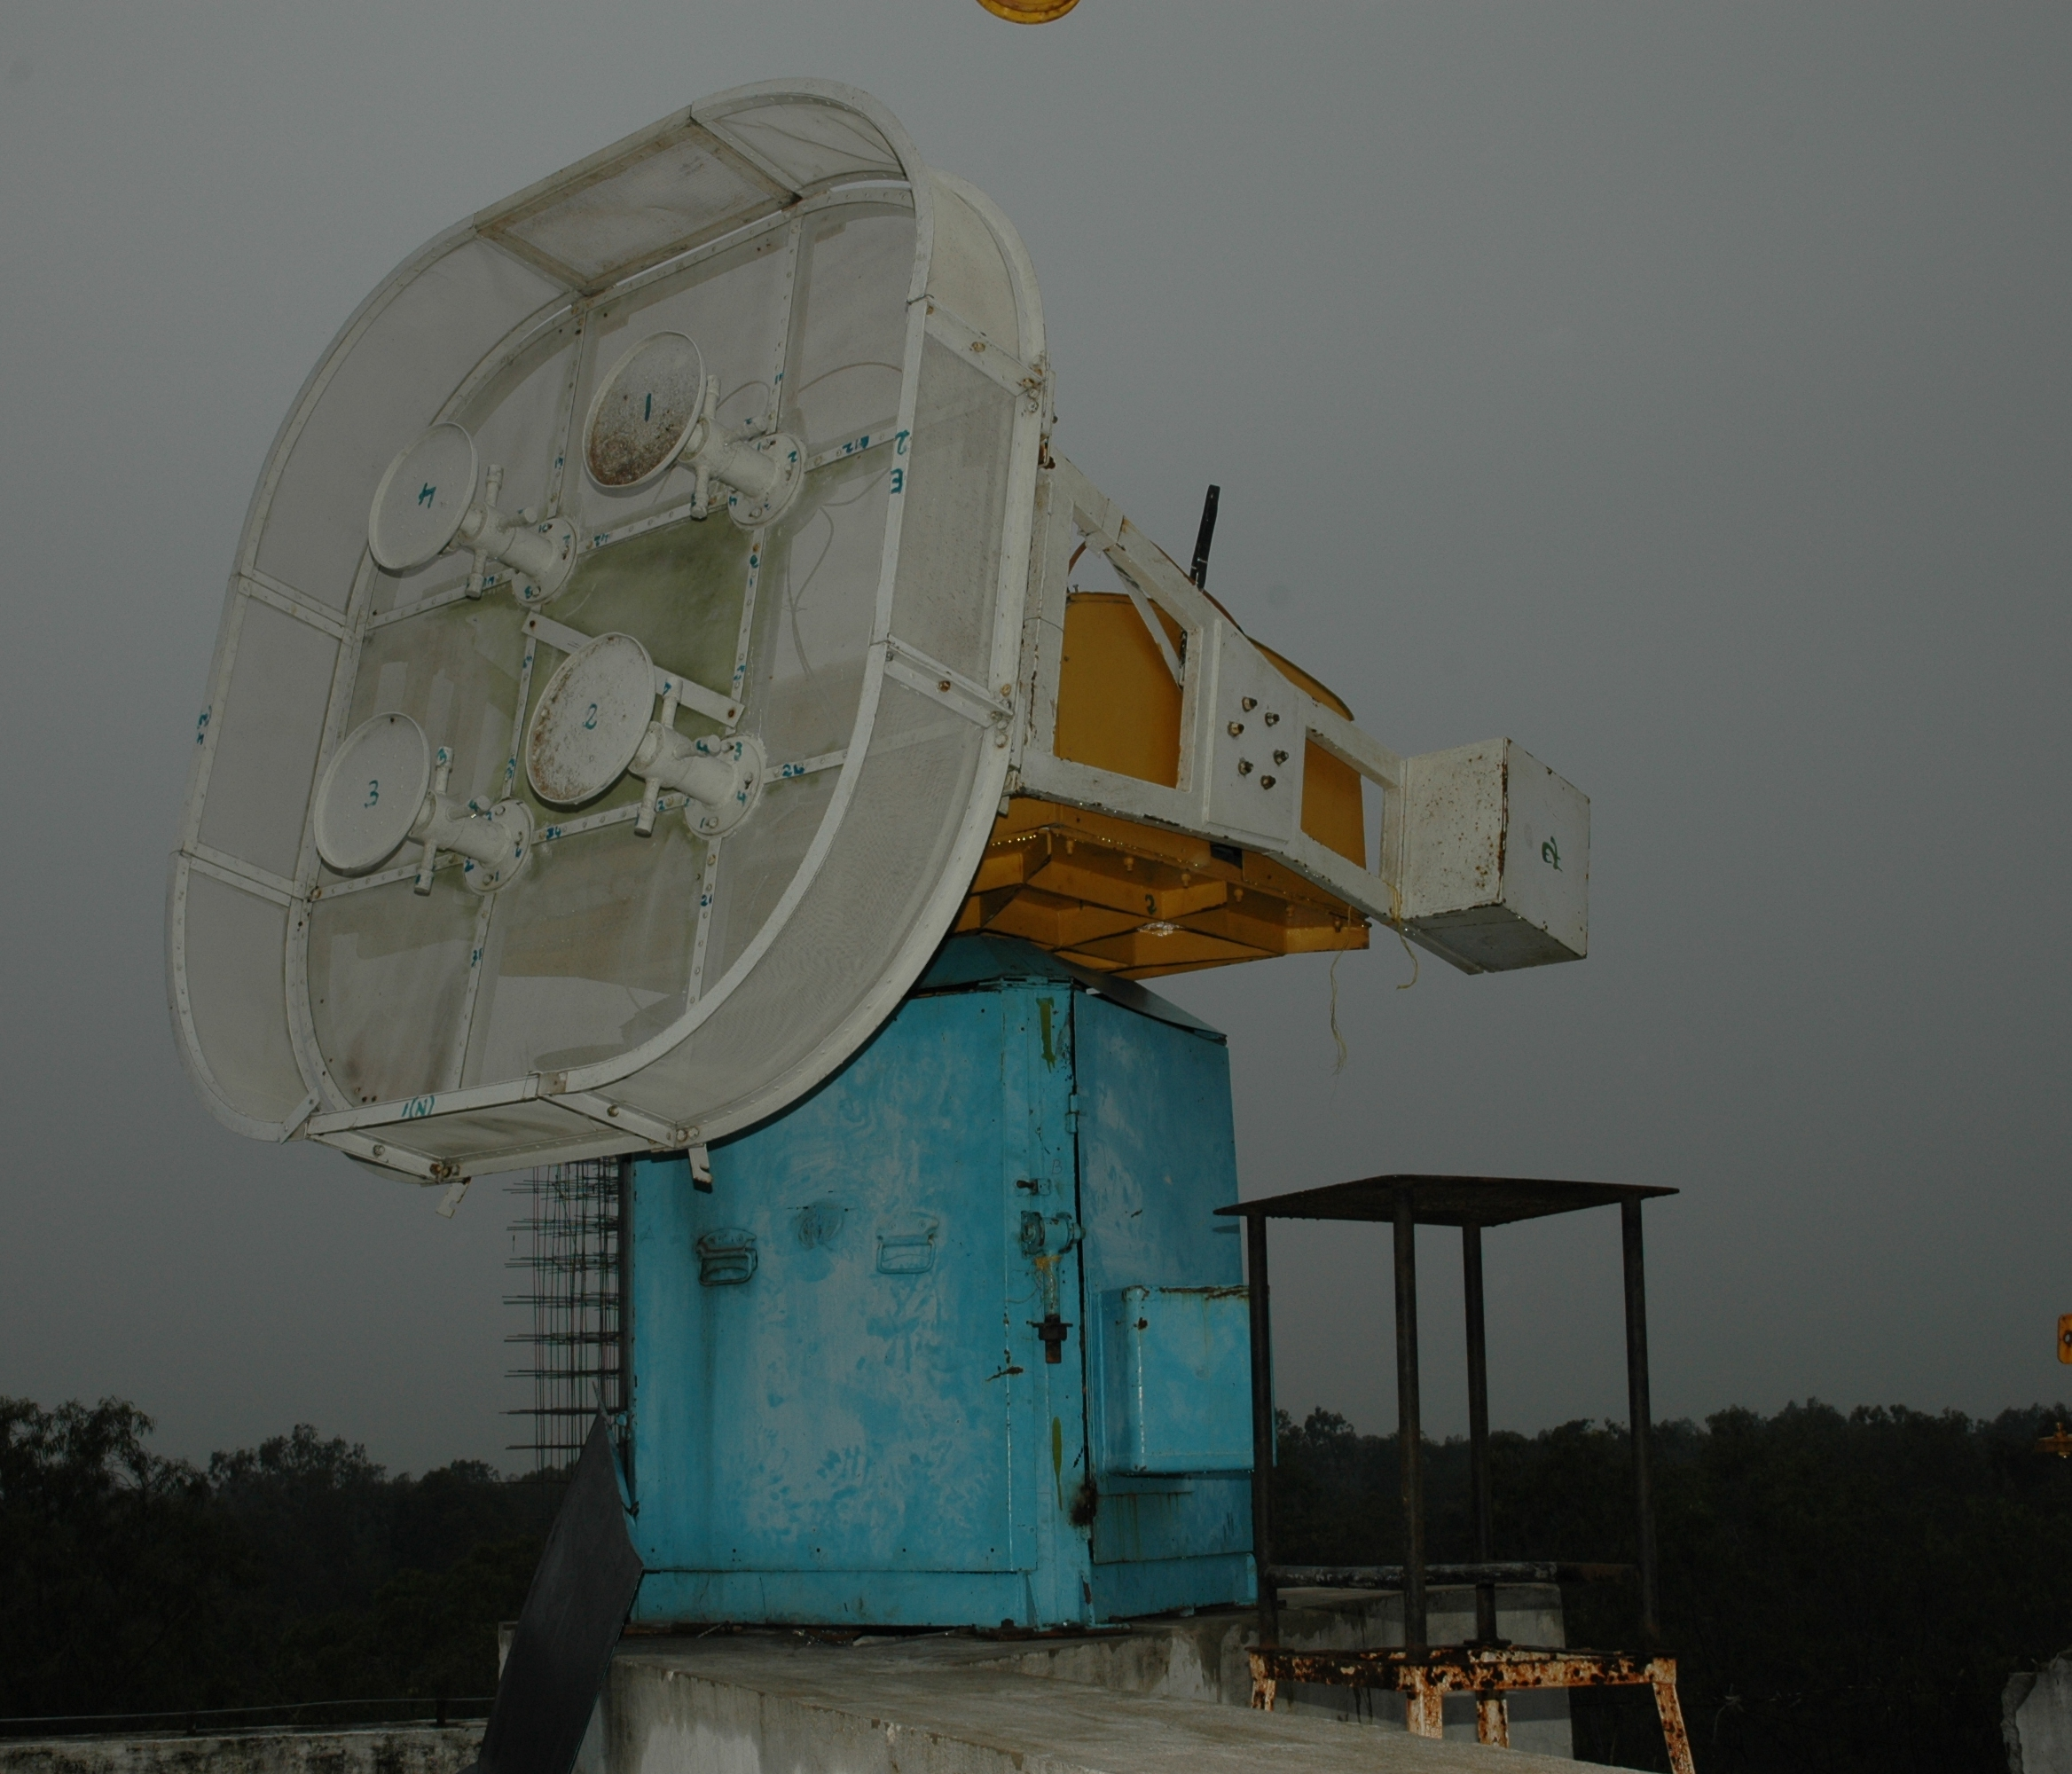
\includegraphics[height=1.5in, width=1.65in]{./AntElement.jpg}&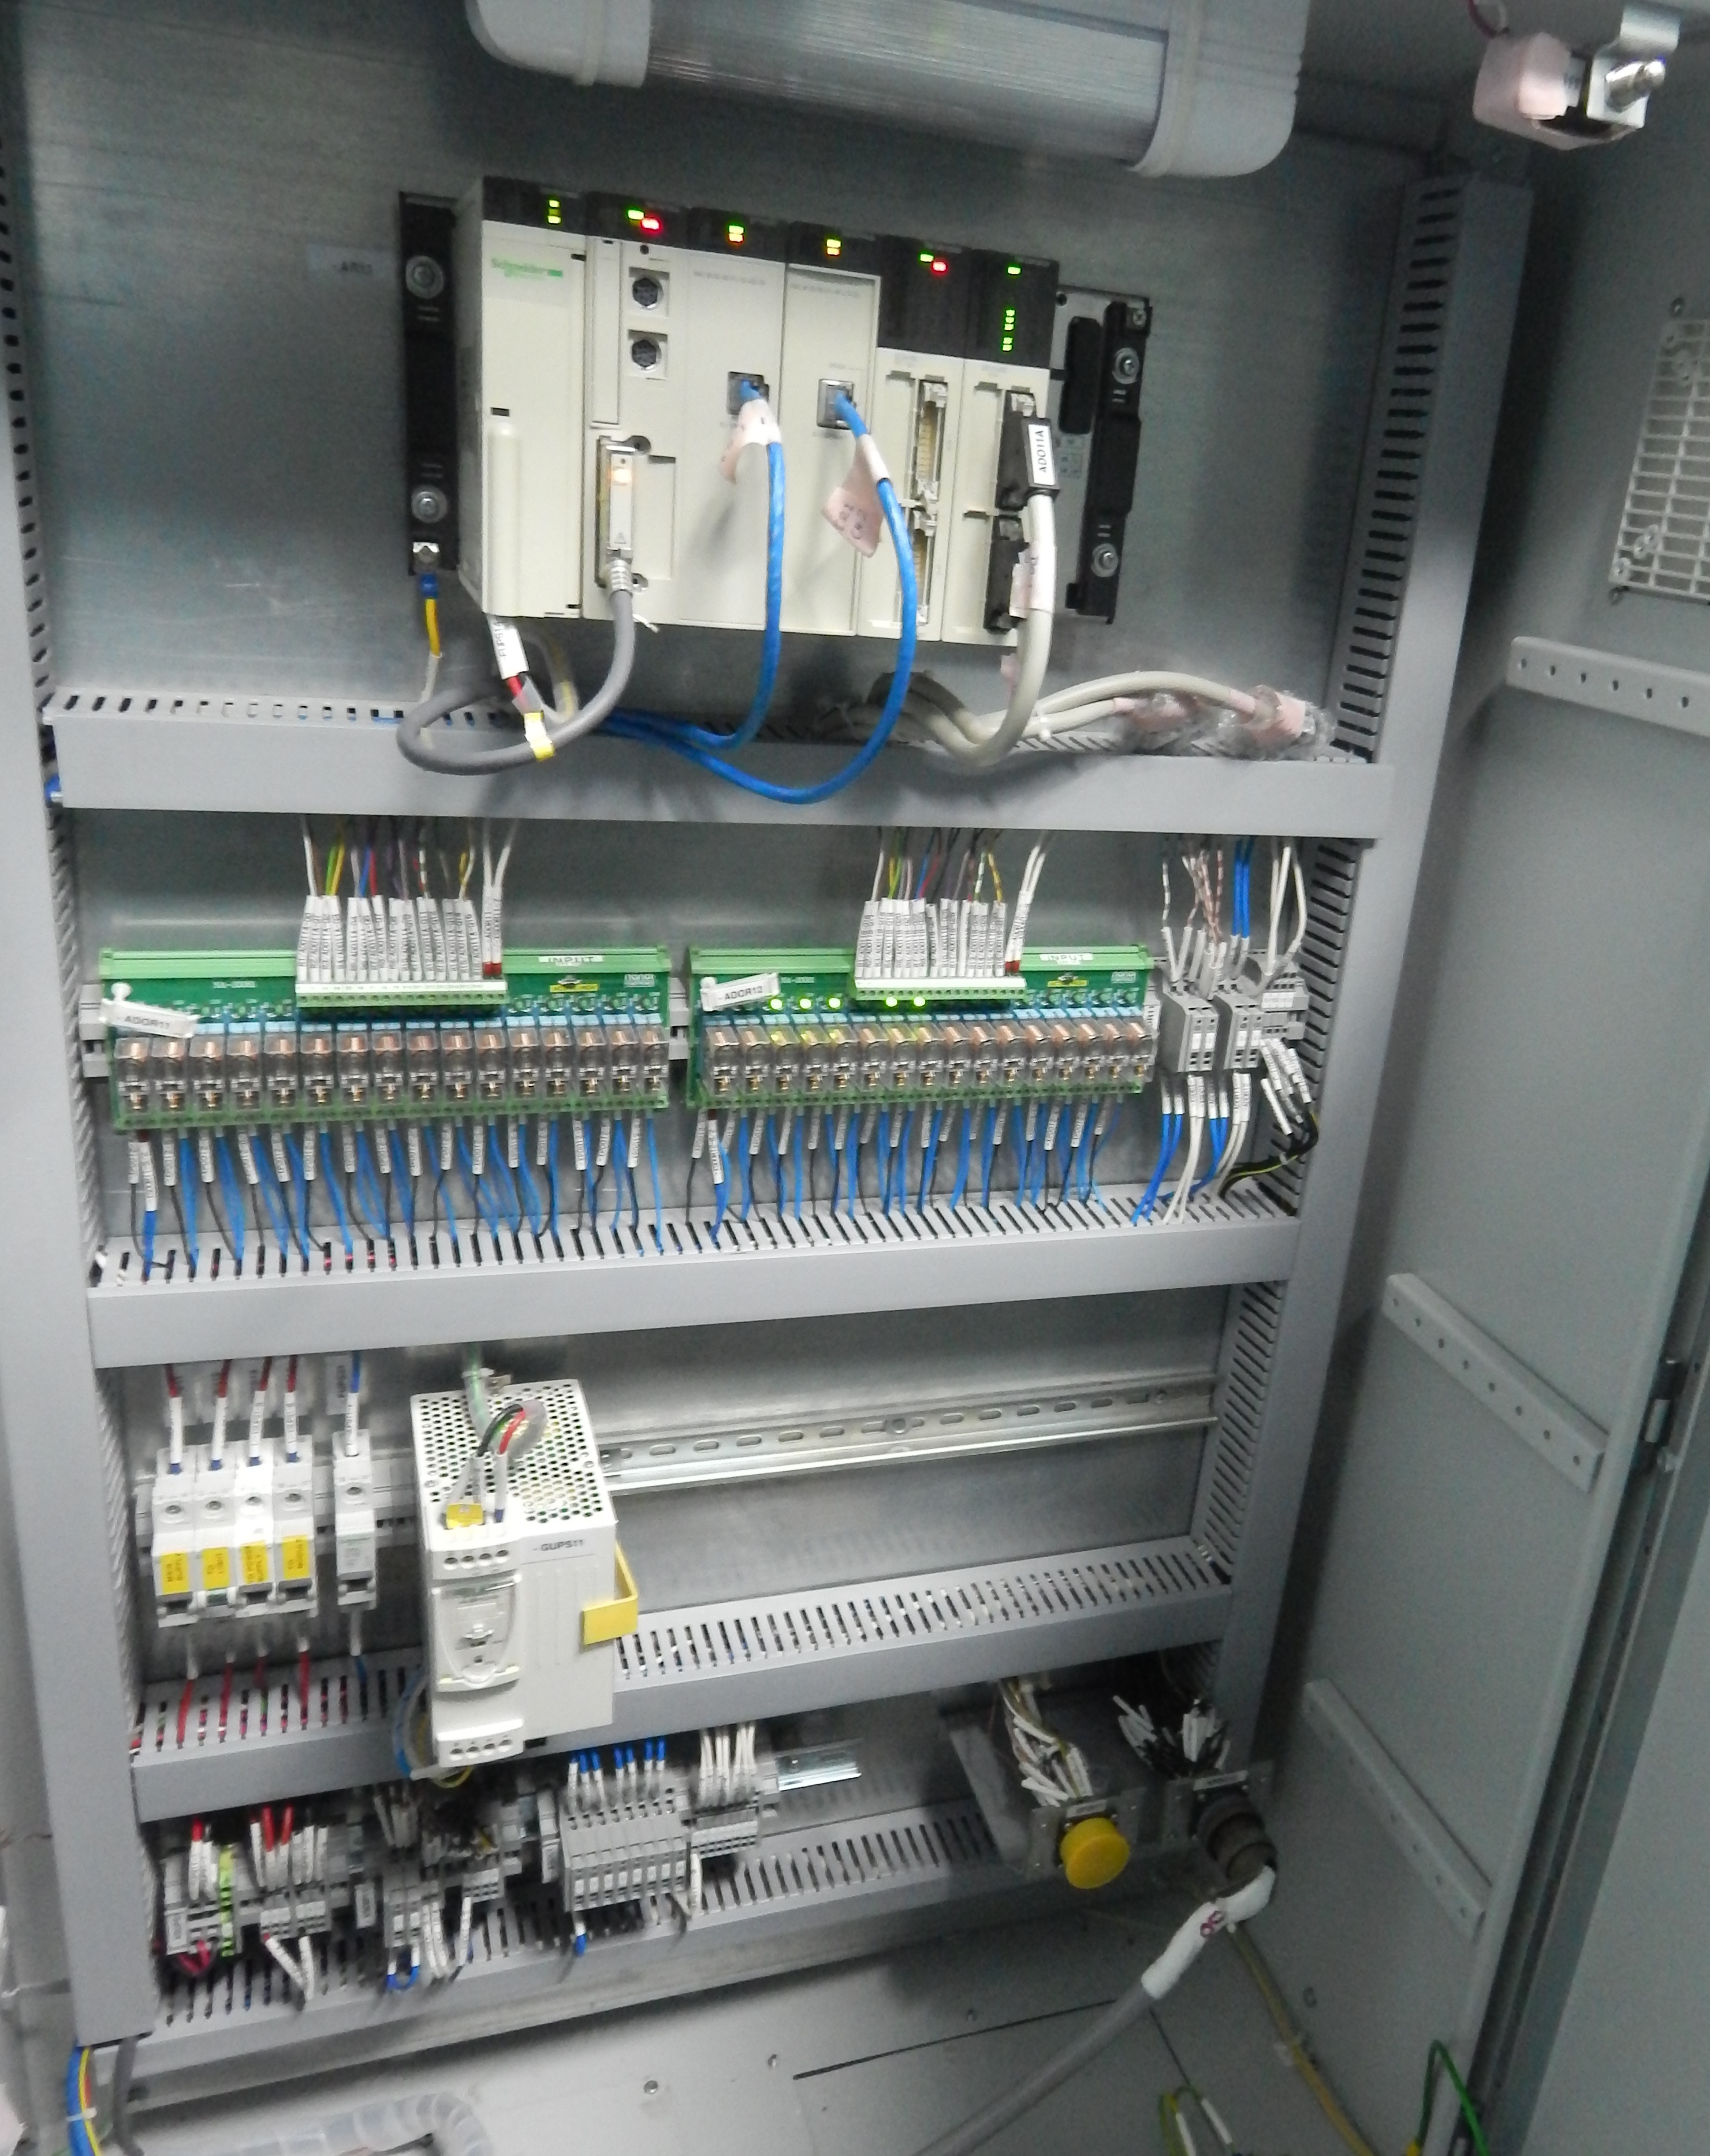
\includegraphics[height=1.5in,width=1.65in]{./CRI1.jpg}&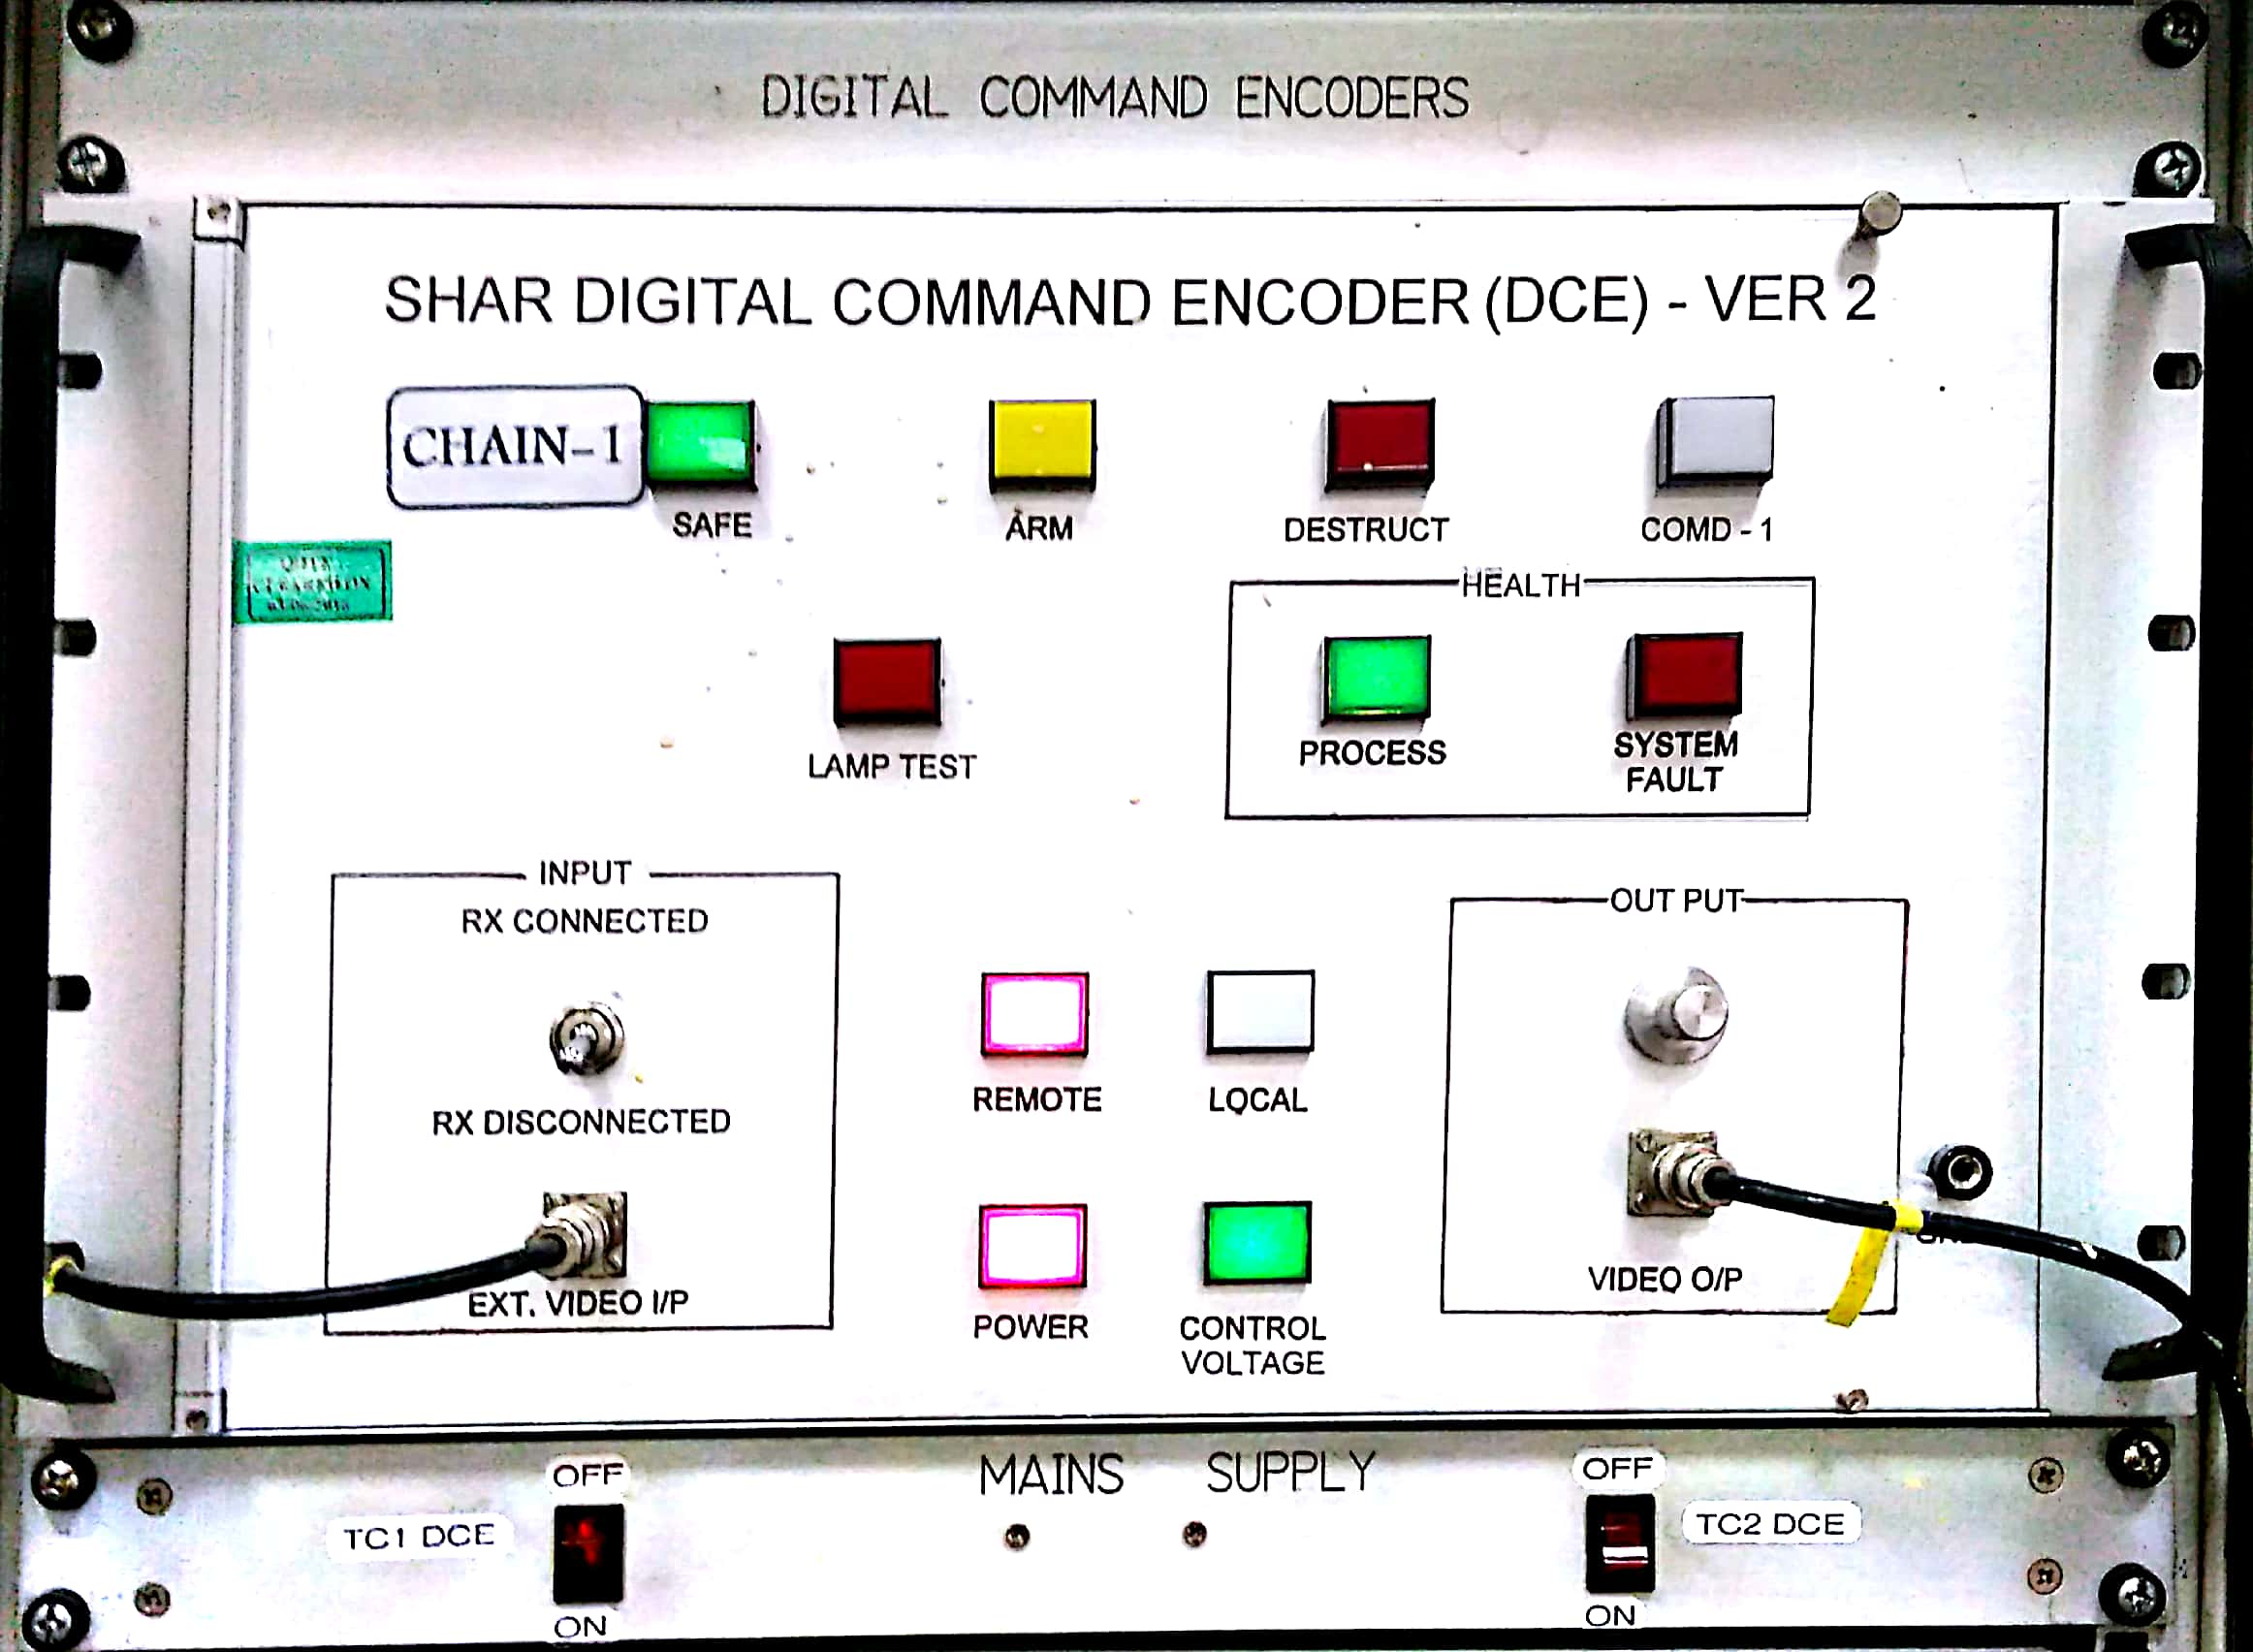
\includegraphics[height=1.5in,width=1.65in]{./DCE.jpg}\\
				
				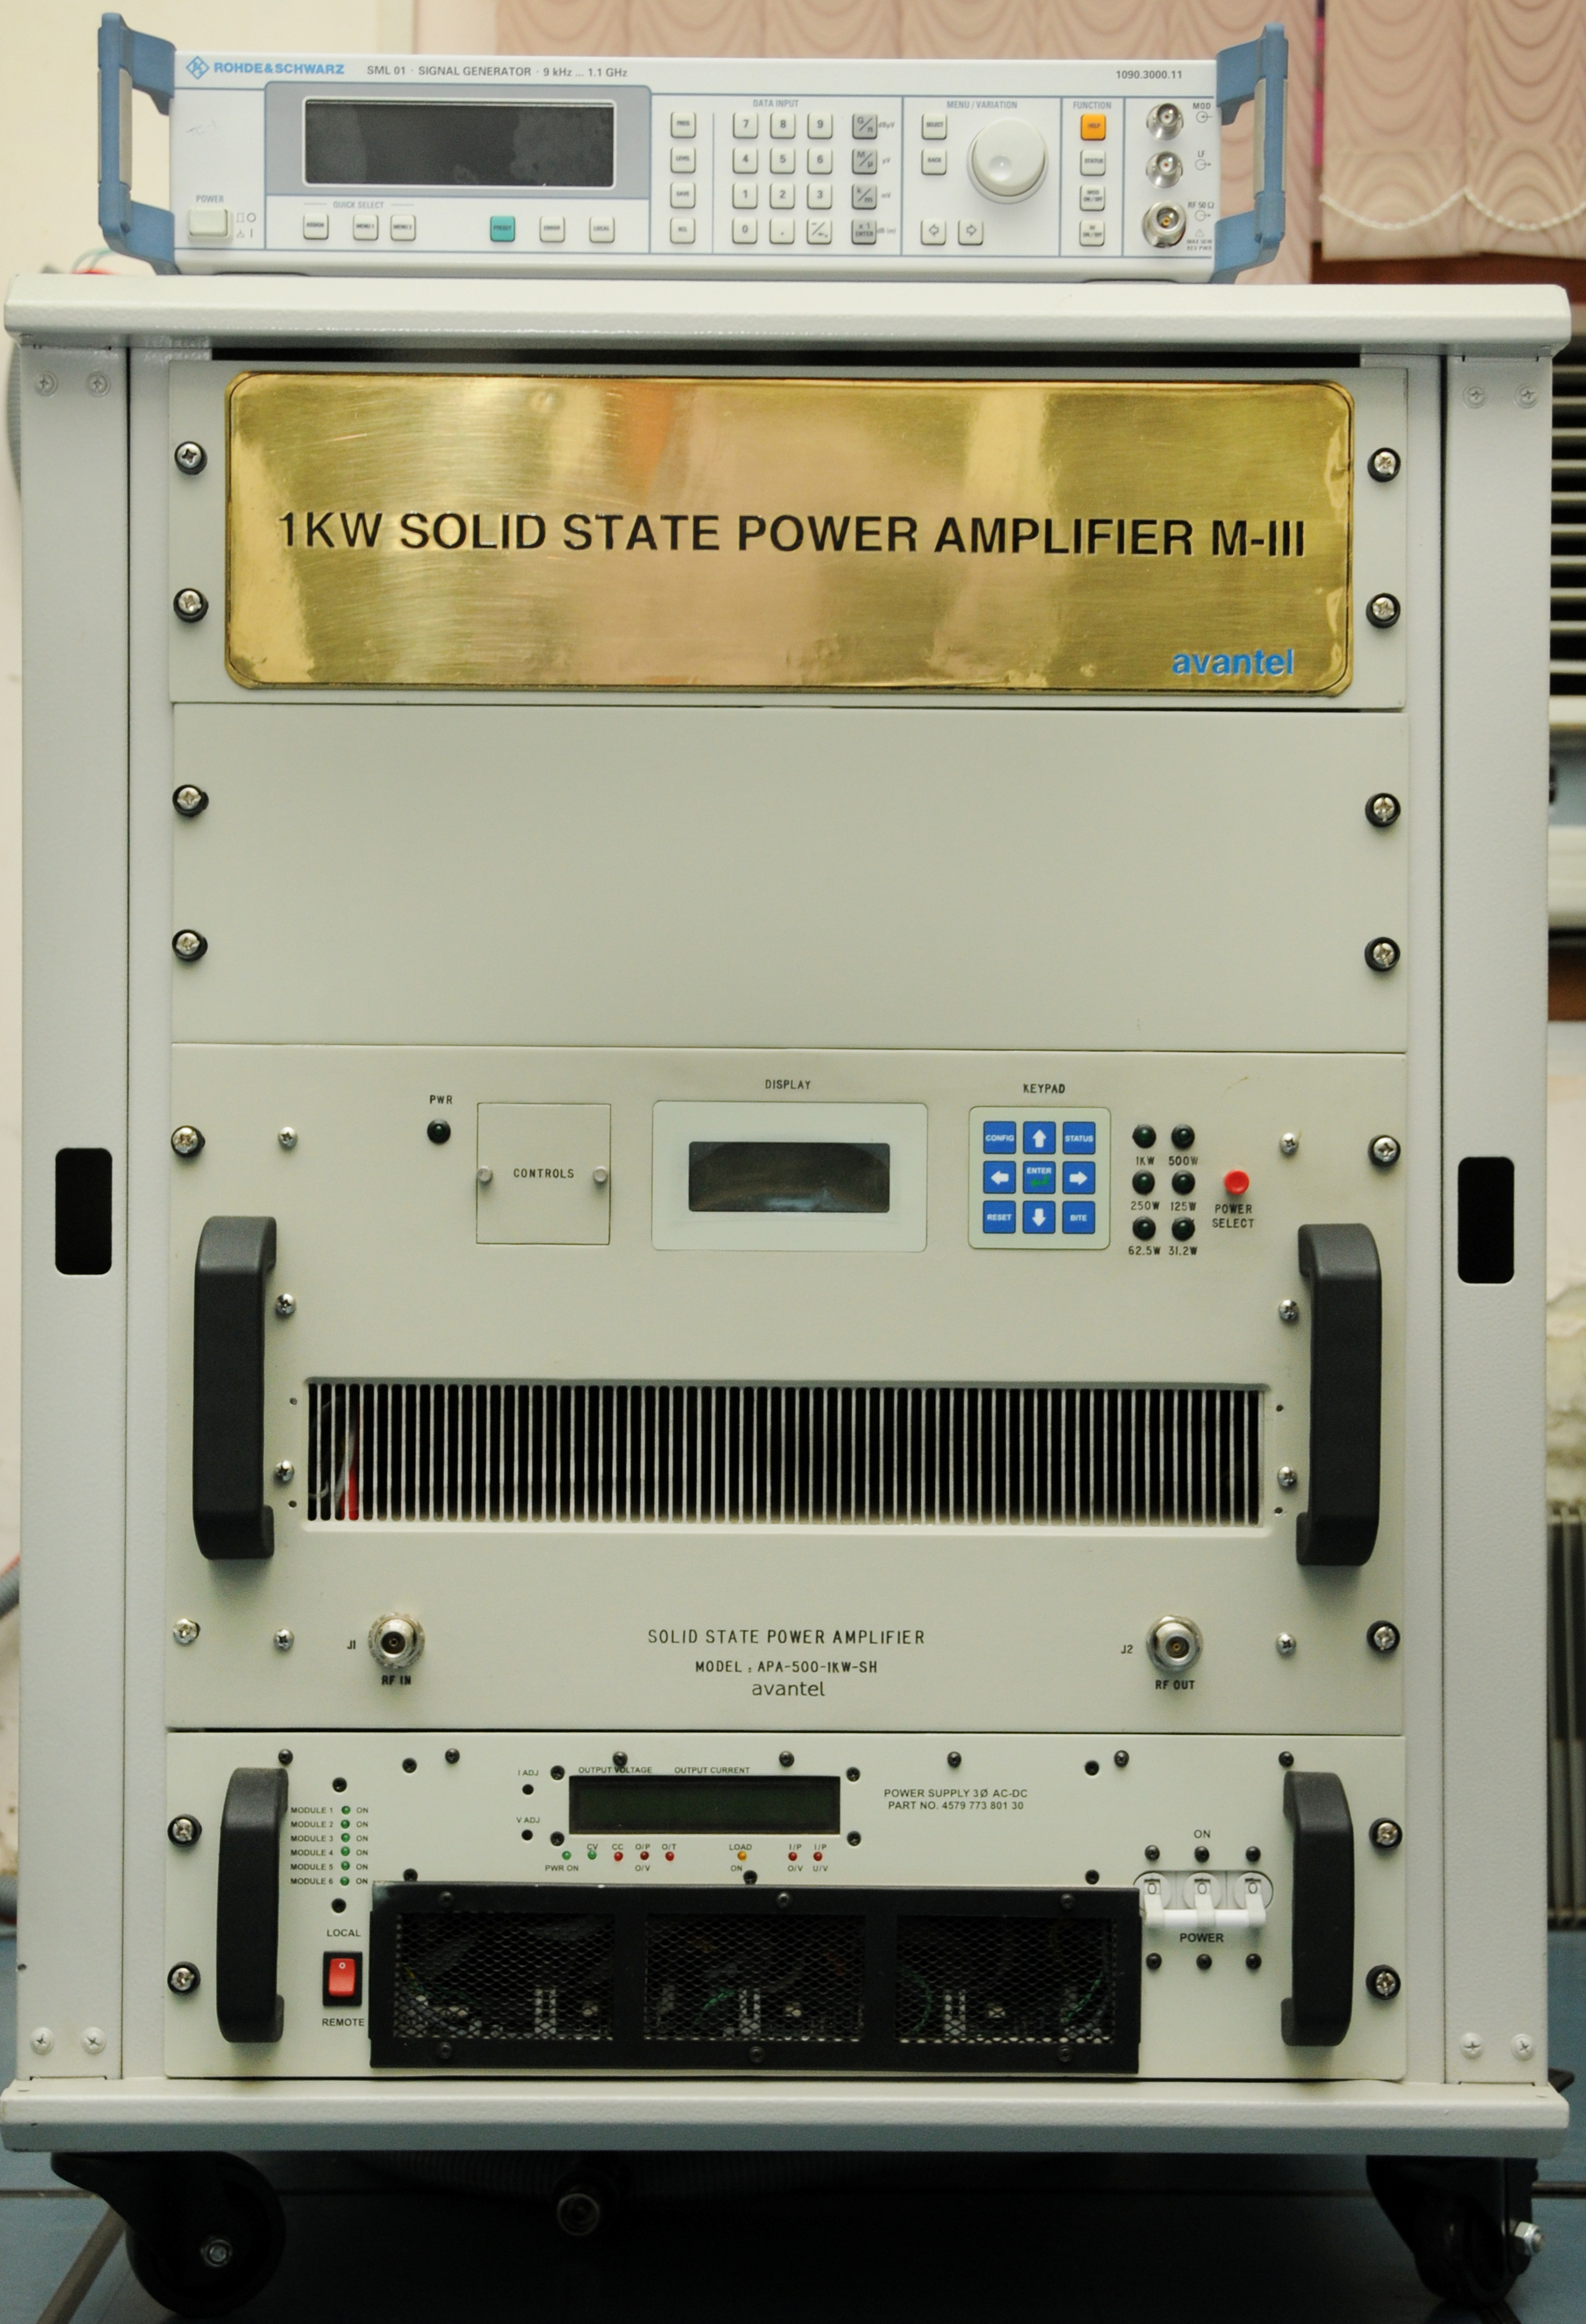
\includegraphics[height=1.5in,width=1.65in] {./NewPA.jpg}&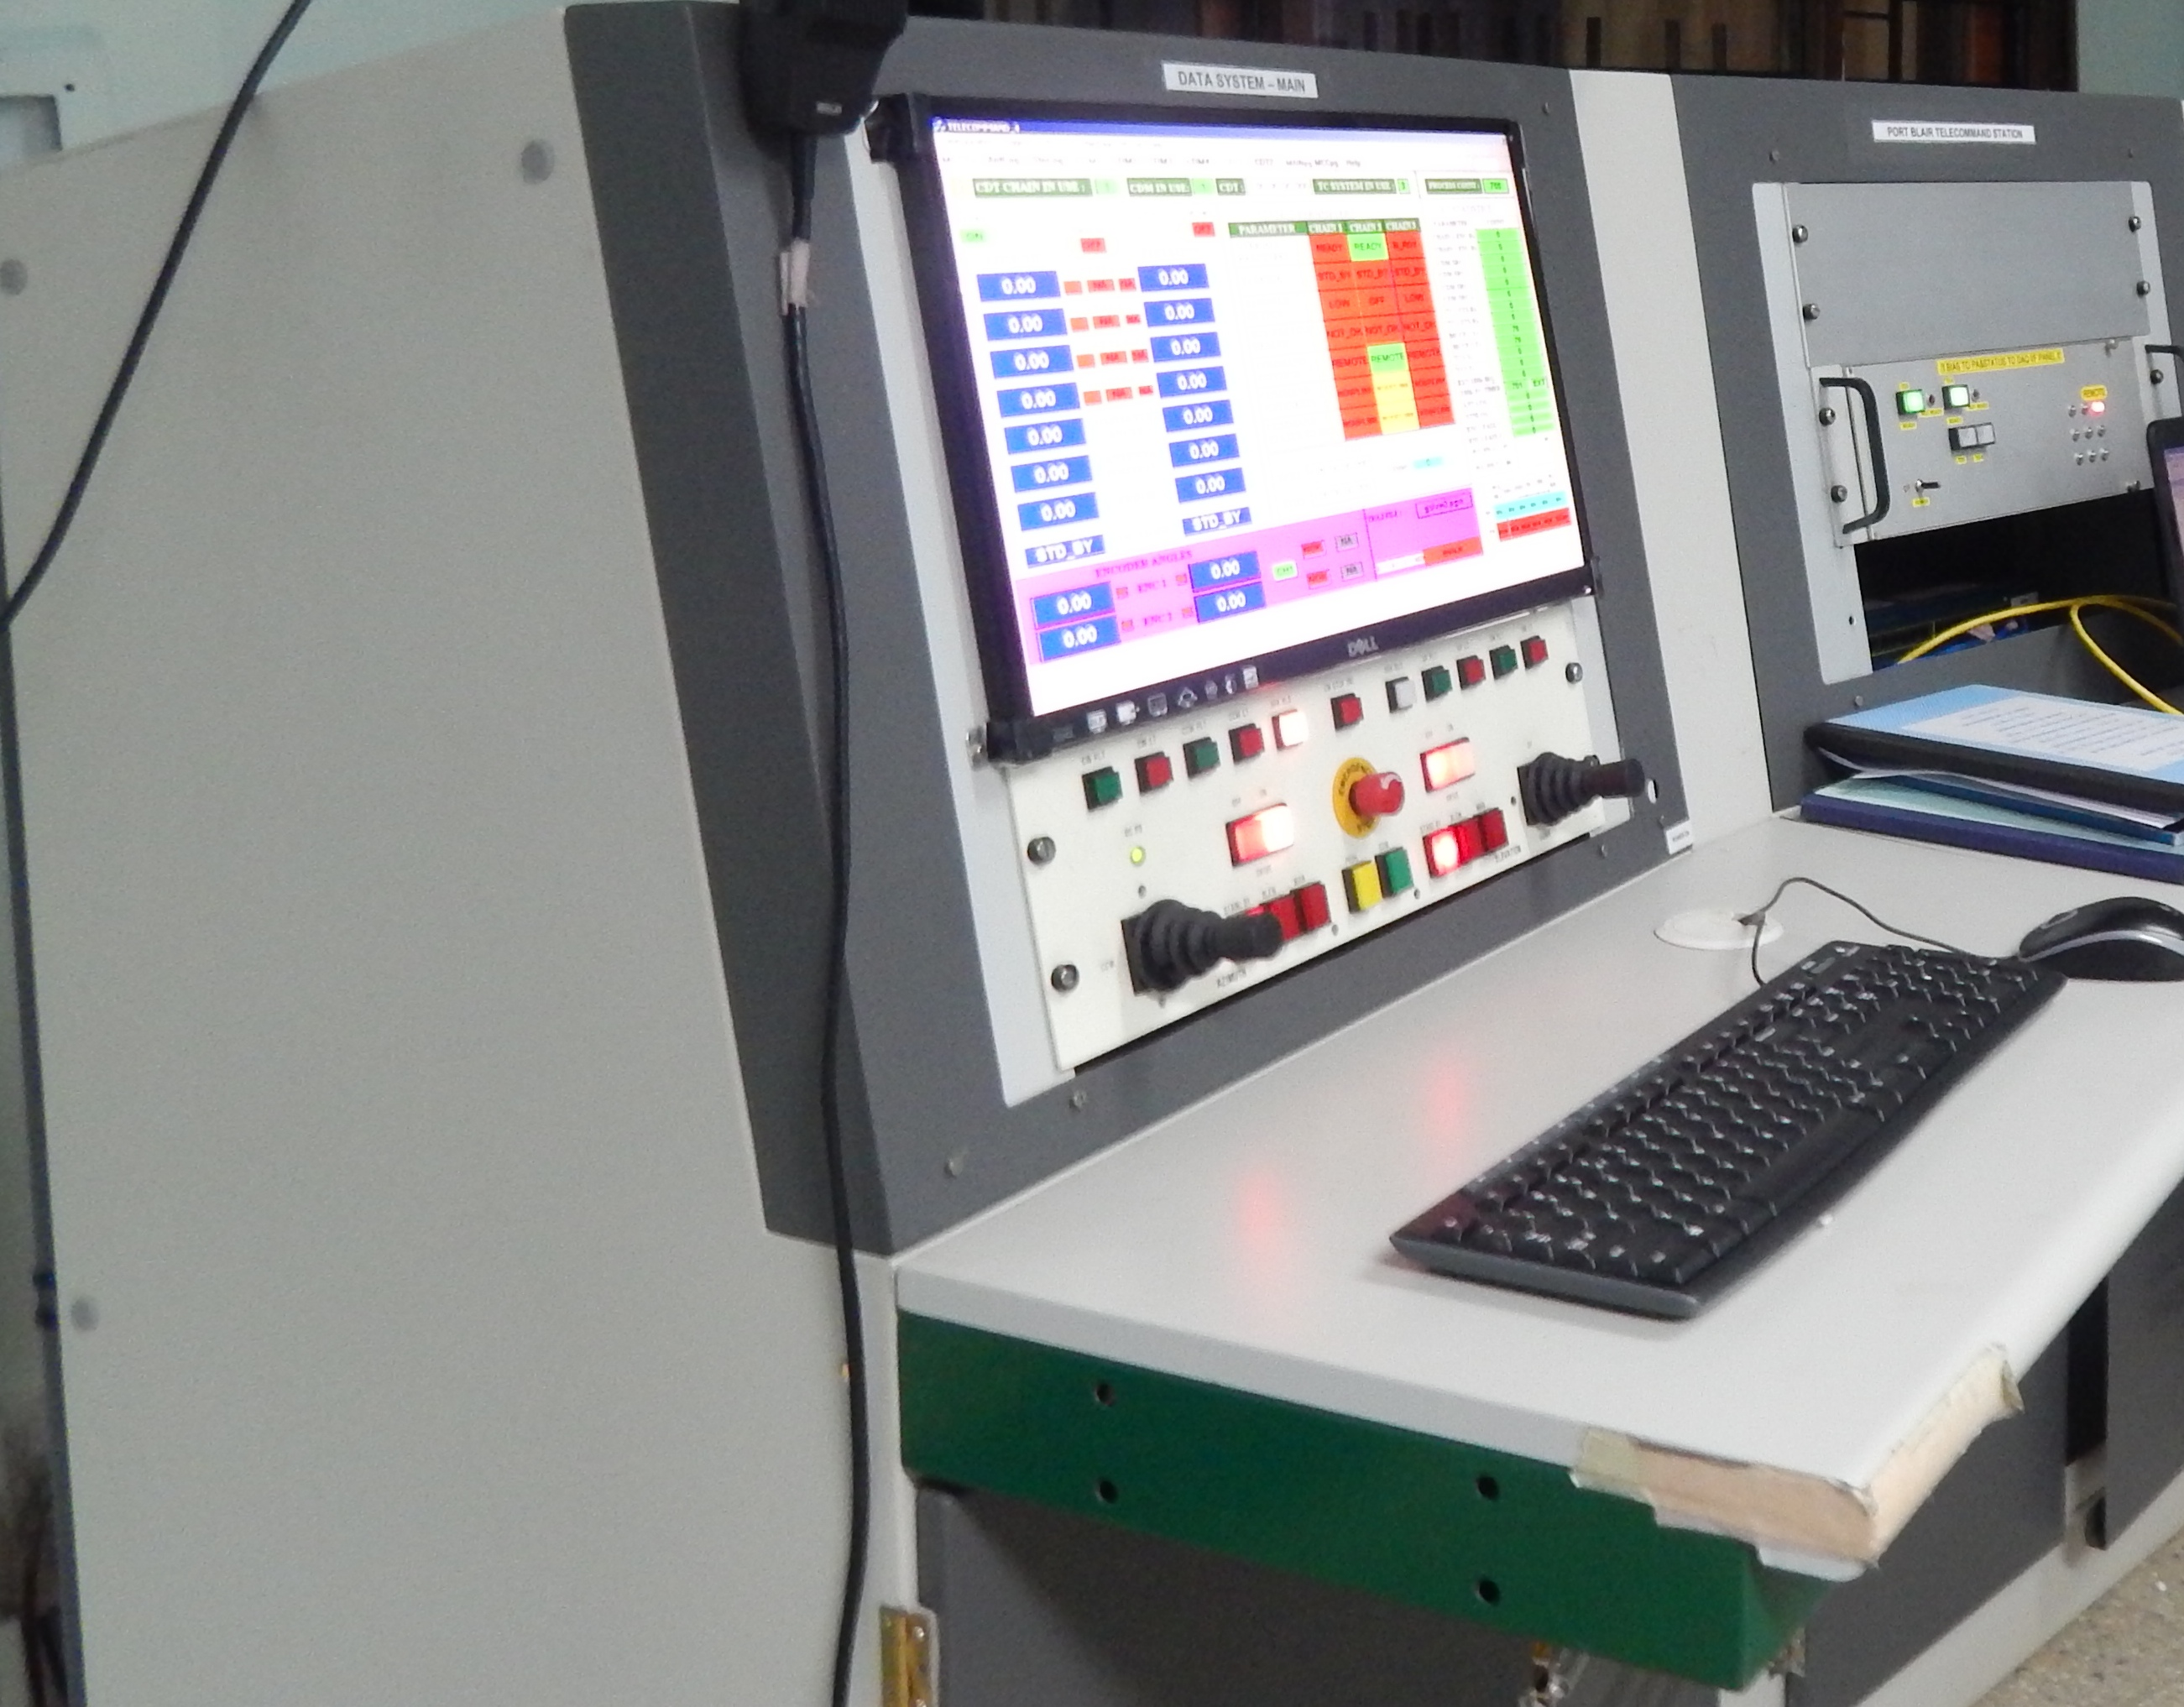
\includegraphics[height=1.5in,width=1.65in]{./Console1.jpg}&\includegraphics[height=1.5in,width=1.65in]{./MainPage.png}\\
				
			\end{tabular}
			
		\end{figure}
		
		\vspace*{0.25in}
		
	\end{center} 
	\begin{center}
		{\bf \large \MakeUppercase{ TIMING}\par} 
		{\hspace*{0.4in} \bf ELECTRONIC INSTRUMENTATION SYSTEMS \newline RANGE OPERATIONS\\
			SATISH DHAWAN SPACE CENTER}
		\vglue 0.50em
		{\bf \large October 2020\par }%\@date}\par
	\end{center}
	%\parskip 8pt
	
	
	
	
	%%%%%%%%%%%%%%%%%%%%%%%%%%%%%%%%%%%%%%%%%%%%%%%%%%%%%%%%%%%%%%%%%%%%%%
	%\newpage
	%\input{certificate}
	\newpage
	\vspace*{36pt}
	\begin{center}
		
		
		\let \footnote \thanks
		\vglue 0in % this makes top margin 2in
		%\vskip 5ex%
		\begin{spacing}{1}
			\textbf{\Large  PC BASED TIMING SYSTEM DEVELOPMENT PROJECT}
		\end{spacing}
		
	\end{center}  
	%\vskip 25pt
	%\thispagestyle{empty}
	
	%\setcounter{page}{0}
	\pagenumbering{roman}
	
	
	\noindent 
	
	
	
	
	\vspace*{1in}
	
	\parbox{1.8in}
	{
		\noindent {\bf Prepared By} \\
		\noindent {\bf } \\
		\noindent             SVK CHAITANYA \\ 
		\noindent Engineer-SD\\
		\noindent TIMING/EIS/RO\\
	} 
	\hspace*{0.20in} 
	\parbox{1.5in}
	{
		\noindent {\bf} \\
		
		\noindent             M PRAVEENA\\ 
		\noindent Engineer-SC\\
		\noindent TIMING/EIS/RO\\
		
		
	}  
	
	
	\vspace*{0.25in}
	
	\parbox{2.2in}
	{
		\noindent {\bf} \\ \\
		\noindent {\bf Checked $\&$ Verified By} \\
		\noindent {\bf} \\
		\noindent             K MALINI \\ 
		\noindent Dy.Manager\\
		\noindent TIMING/EIS/RO\\
		\noindent {\bf} \\
		\noindent {\bf} \\
	} 
	\parbox{2.2in}
	{
	\noindent {\bf } \\
	\noindent {\bf } \\
	\noindent J GOPALAKRISHNA \\ 
	\noindent General Manager\\
	\noindent EIS/RO\\
	} 
\hspace*{0.20in} 
	
	\vspace*{0.25in}
	
	\parbox{2.2in}
	{
		\noindent {\bf Reviewed \& Approved By} \\
		\noindent {\bf} \\
		\noindent             G.GRAHADURAI \\ 
		\noindent Chairman\\
		\noindent STARS\\
	} 
	\newline
	\hspace*{2.5in}
	\noindent Sriharikota\\
	\hspace*{2.4in}
	October, 2020
	\clearpage
	%%---------------------------------------------\clearpage
	\vspace*{36pt}
	%\declaration
	\begin{center}
		{\large \bf CERTIFICATE}
	\end{center}
	
	
	\vspace*{24pt}
	
	% Please add the following required packages to your document preamble:
	% \usepackage{booktabs}
	\begin{table}[h]
		\centering
		%	\caption{Certificate}
		\label{TAB:Certificate}
		\begin{tabular}{@{}lll@{}}
			\toprule
			\textbf{Sl No} & \textbf{Parameter}           & \textbf{Description}                           \\ \midrule
			1              & Security                     & \textbf{Restricted}                            \\
			2              & Status                       & \textbf{Revised}                                   \\
			3              & Document No                  & ISRO-SHAR-03-R-TR-168-2017                              \\
			4              & Type of Document             & TR - Technical Report                          \\
			5              & Title \& Sub-title           & Software Design Document for \\
			&                              & PC Based TIMING System           \\
			6              & Author(s)                    & SVK CHAITANYA, Engineer-SD, TIMING/EIS/RO \newline    \\
			&                              & M PRAVEENA, Engineer-SC, TIMING/EIS/RO           \\
			                             
			7              & Checked $\&$ Verified   & K MALINI , Dy.Manager, TIMING/EIS/RO           \\                  
			& & J Gopalakrishna, General Manager, EIS/RO      \\
			8              & Reviewed                     & STARS                                          \\
			9              & Approved                     & STARS                                          \\
			10             & Originating Agency           & Satish Dhawan Space Center, SDSC SHAR          \\
			11             & Month \& Year of Publication & October, 2020                                  \\
			12             & No. of Pages                 & 16+186                                             \\
			13             & No. of Figures               & 12                                             \\
			14             & No. of Tables                & 09                                             \\
			15             & No. of References            & 06                                             \\
			16             & No. of Enclosures            & Verification\&Validation, Test\&Evaluation document                                            \\ \bottomrule
		\end{tabular}
		
		
	\end{table}
	
	\parbox{2.9in}{
		
	}  
	
\clearpage
%%---------------------------------------------
\clearpage
\vspace*{36pt}
%\declaration
\begin{center}
{\large \bf CHANGE HISTORY}
\end{center}


\vspace*{24pt}

% Please add the following required packages to your document preamble:
% \usepackage{booktabs}
\begin{table}[h]
	\centering
	%	\caption{Certificate}
	\label{TAB:Certificate}
	\begin{tabular}{@{}lll@{}}
		\toprule
		\textbf{Sl No} & \textbf{Parameter}           & \textbf{Description}                           \\ \midrule
		1              & Project Name           & Software Design Document (SDD) of \\
		&                              & PC Based TIMING Systems           \\
		2              & Plan Version No                      & 1.0      \\
		3              & Date of release                   & 12-10-2020                                          \\
		4              & Approved by                     & STARS                                          \\
		             & Signature          &           \\
		5            & No. of pages &  NA                                 \\
		6             & List of pages for changes made                 &   NA                                         \\
		7             & List of previous version Nos      &  NA                                            \\
		8             & Dates of release of previous versions     &  NA                \\
		 \bottomrule
	\end{tabular}
	
	
\end{table}
\parbox{2.9in}

\vspace*{0.25in}

%%%%%%%%%%%%%%%%%%%%%%%%%%%%%%%%%%%%%%%%%%%%%%%%%%%%%%%%%%%%%%%%%%%%%



\setstretch{1.3}  % It is better to have smaller font and larger line spacing than the other way round

% Define the page headers using the FancyHdr package and set up for one-sided printing
\fancyhead{}  % Clears all page headers and footers
\rhead{\thepage}  % Sets the right side header to show the page number
\lhead{}  % Clears the left side page header

\pagestyle{fancy}  % Finally, use the "fancy" page style to implement the FancyHdr headers

%% ----------------------------------------------------------------

%%%%%%%%%%%%%%%%%%%%%%%%%%%%%%%%%%%%%%%%%%%%%%%%%%%%%%%%%%%%%%%%%%%% ----------------------------------------------------------------
\clearpage  % Declaration ended, now start a new page
% The Abstract Page
\setstretch{1.4}


%\abstract{

\addtocontents{toc}{\vspace{0em}}
\begin{center}
\LARGE\textit{Abstract}
\end{center}
\vspace{-3 mm}
\begin{spacing}{1.3}

Development of PC based TIMING System is being carried out. This document describes the Software Design Documetn (SDD) for  PC based TIMING  System Development. The base line reference for the preparation of this document are TIMING DATA SYSTEM software design document \cite{TCOldSWDoc}, and PC based Timing system software requirements document \cite{SRSLBDPS}. \\

PC based Timing  System takes Four time codes namely  UT-1,UT-2,CDT-1,CDT-2. as input via PCI park control time code reader cards and Transmits the time information acquired from all cards as Ethernet Packet\\

This document is made as per the guidelines of the ISPD and follows the IEEE STD 1233-1998. The document is organized as 10 sections. Section \ref{Chapter1} describes purpose of the system and its sub-systems. It also presents the scope and over view of the entire system. In section \ref{Chapter2}, decomposition descripton is given. This includes module level decomposition, concurrent process decomposition and data decomposition. Dependency description which includes intermodule dependency, interprocess dependency and data dependencies, is provided in section \ref{Chapter3}. Interface description  of module and process are given in section \ref{Chapter4}. Detailed design containing modules detailed design, threads detailed design, data detailed design are explained in section \ref{Chapter5}. Section \ref{Chapter6} gives the procedures for loading OS and add on drivers along with useful commands. Details of various data logging formats, interconnections, configuration files and pin assignments are presented in section \ref{Chapter7}. Flow charts are given in section \ref{Chapter8} which details the flow of code. Section \ref{Chapter9} presents the features of new linux based Data Systems compares to that of old windows 2K based Data Systems. Finally, section \ref{Chapter10} provides the GUI pages  of linux Data System with description.



\end{spacing}

\clearpage  % Abstract ended, start a new page
%% ----------------------------------------------------------------
\setstretch{1.4}


%\abstract{

\addtocontents{toc}{\vspace{0em}}
\begin{center}
\LARGE\textit{Keywords}
\end{center}
\vspace{10 mm}
\begin{spacing}{1.5}


%Probabilistic Models \\
%Boltzmann Machines \\
Graphical User Interface\\
Absolute Rotary Encoder\\
Linux Operating System\\ 
Serial Communication\\
Digital Command Encoder Unit\\  
Amplifier Bias\\
Control Panel\\
Range Safety\\
Receiver\\
Antenna\\
Driver Amplifier\\
Demodulator\\
Convolutional Encoder\\
Viterbi Decoder\\
\end{spacing}

\clearpage  % keywords Ended here
%% ----------------------------------------------------------------


%\addtocontents{toc}{\vspace{0em}}
%\begin{center}
%\LARGE\textit{Acronyms}
%\end{center}
%\vspace{10 mm}
%\begin{spacing}{1.5}
%CNN\:			: Convolutional Neural Network\\
%DL\:			: Deep Learning\\
%RBM\:			: Restricted Boltzman Machine\\
%FBP\:			: Feed Back Propagation\\
%WM\:			: WaterMark\\
%CB\:			: Code Book\\
%DCT\:			: Discrete Cosine Transform\\
%DWT\:			: Discrete Wavelet Transform\\
%SVD\:			: Singular Value Decomposition\\
%SWT\:			: Stationery Wavelet Transform\\
%
%
%			
%\end{spacing}
%
%\clearpage  % Acronyms Ended here
 ----------------------------------------------------------------

\setstretch{1.5}  % Reset the line-spacing to 1.3 for body text (if it has changed)

% The Acknowledgements page, for thanking everyone

\acknowledgements{
\addtocontents{toc}{\vspace{1em}}  % Add a gap in the Contents, for aesthetics
 
\paragraph*{}  
%We express our sincere gratitude to Dr. Sai Subrahmanyam Gorthi, Associate Professor, IIST and Dr Deepak Mishra, Associate Professor, IIST for their guidance, enthusiastic encouragement for completion of this thesis work. I am grateful for the assistance provided by them. I would like to offer my special thanks to them for providing me with this golden opportunity to do this work which helped me in learning a lot of things.\\ 

We like to thank Smt G Krishna kumari, Manager, Timing , who Structured and Coded the Project . \\ 
We specially like to thank Sri V Dillep ,Eng-SE, TIMING ,A Munaswamy, A Abilash and Shamna ,Tehcnician for helping us in realising terminations and Testing  works.\\

We like to express our heartful thanks to Sri G Grahadurai, DD, RO for guiding us through the phases of development with continuous reviews and suggestions. We also like to thank the sub-committee members of STARS i.e., Sri C Ramsenthil, Sri K V Dinesh Babu, Sri K Vishnu Vardhan Reddy for thorough code walk through and valuable inputs in further improving the design. We also like to thank all the members of STARS for their valuable time in reviewing the design in every aspect and made the product more reliable.\\
We express our sincere gratitude to  Sri J Gopalakrishana, GM, RIS; for their continuous encouragement for the successful realisation of the PC based TIMING system. \\

}
\clearpage  % End of the Acknowledgements
\frontmatter      % Begin Roman style (i, ii, iii, iv...) page numbering
\begin{comment}
% Set up the Title Page
\title  {Deep Learning Methods and Applications }
\authors  {\texorpdfstring
            {\href{hari.friends.4u@gmail.com}{Haribabu Kandi}}
            {Haribabu Kandi}
            }
\addresses  {\groupname\\\deptname\\\univname}  % Do not change this here, instead these must be set in the "Thesis.cls" file, please look through it instead
\date       {\today}
\subject    {}
\keywords   {}

	\maketitle
%% ----------------------------------------------------------------

\setstretch{1.3}  % It is better to have smaller font and larger line spacing than the other way round

% Define the page headers using the FancyHdr package and set up for one-sided printing
\fancyhead{}  % Clears all page headers and footers
\rhead{\thepage}  % Sets the right side header to show the page number
\lhead{}  % Clears the left side page header

\pagestyle{fancy}  % Finally, use the "fancy" page style to implement the FancyHdr headers

%% ----------------------------------------------------------------
% Declaration Page required for the Thesis, your institution may give you a different text to place here
%\Declaration{

%\addtocontents{toc}{\vspace{1em}}  % Add a gap in the Contents, for aesthetics

%I, AUTHOR NAME, declare that this thesis titled, `THESIS TITLE' and the work presented in it are my own. I confirm that:

%\begin{itemize} 
%\item[\tiny{$\blacksquare$}] This work was done wholly or mainly while in candidature for a research degree at this University.
 
%\item[\tiny{$\blacksquare$}] Where any part of this thesis has previously been submitted for a degree or any other qualification at this University or any other institution, this has been clearly stated.
 
%\item[\tiny{$\blacksquare$}] Where I have consulted the published work of others, this is always clearly attributed.
 
%\item[\tiny{$\blacksquare$}] Where I have quoted from the work of others, the source is always given. With the exception of such quotations, this thesis is entirely my own work.
 
%\item[\tiny{$\blacksquare$}] I have acknowledged all main sources of help.
 
%\item[\tiny{$\blacksquare$}] Where the thesis is based on work done by myself jointly with others, I have made clear exactly what was done by others and what I have contributed myself.
%\\
%\end{itemize}
 
 
%Signed:\\
%\rule[1em]{25em}{0.5pt}  % This prints a line for the signature
 
%Date:\\
%\rule[1em]{25em}{0.5pt}  % This prints a line to write the date
%}
%\clearpage  % Declaration ended, now start a new page

%% ----------------------------------------------------------------
% The "Funny Quote Page"
%\pagestyle{empty}  % No headers or footers for the following pages

%\null\vfill
% Now comes the "Funny Quote", written in italics
%\textit{``Write a funny quote here.''}

%\begin{flushright}
%If the quote is taken from someone, their name goes here
%\end{flushright}

%\vfill\vfill\vfill\vfill\vfill\vfill\null
\clearpage  % Funny Quote page ended, start a new page
%% ----------------------------------------------------------------

% The Abstract Page
\addtotoc{Abstract}  % Add the "Abstract" page entry to the Contents
\abstract{
\addtocontents{toc}{\vspace{1em}}  % Add a gap in the Contents, for aesthetics

}

\clearpage  % Abstract ended, start a new page
%% ----------------------------------------------------------------

\setstretch{1.3}  % Reset the line-spacing to 1.3 for body text (if it has changed)

% The Acknowledgements page, for thanking everyone
\acknowledgements{
\addtocontents{toc}{\vspace{1em}}  % Add a gap in the Contents, for aesthetics

}
%\clearpage  % End of the Acknowledgements
%%
\end{comment}
%----------------------------------------------------------------

%\pagestyle{fancy}  %The page style headers have been "empty" all this time, now use the "fancy" headers as defined before to bring them back

%% ----------------------------------------------------------------
\lhead{\emph{Contents}}  % Set the left side page header to "Contents"
\tableofcontents  % Write out the Table of Contents

%% ----------------------------------------------------------------
\lhead{\emph{List of Figures}}  % Set the left side page header to "List if Figures"
%%
\listoffigures  % Write out the List of Figures
%%\pagebreak
%%
%%%% ----------------------------------------------------------------
\lhead{\emph{List of Tables}}  % Set the left side page header to "List of Tables"
%%
\listoftables  % Write out the List of Tables
%% ----------------------------------------------------------------
\setstretch{1.3}  % Set the line spacing to 1.5, this makes the following tables easier to read
\clearpage  % Start a new page
\lhead{\emph{Abbreviations}}  % Set the left side page header to "Abbreviations"
\listofsymbols{ll}  % Include a list of Abbreviations (a table of two columns)
{
% \textbf{Acronym} & \textbf{W}hat (it) \textbf{S}tands \textbf{F}or \\
\textbf{DPS}	& \textbf{D}ata \textbf{P}rocessing \textbf{S}ystem \\
\textbf{GUI} 	& \textbf{G}raphical \textbf{U}ser \textbf{I}nterface\\
\textbf{EDAU}	& \textbf{E}ncoder \textbf{D}ata \textbf{A}cquisition \textbf{U}nit\\
\textbf{AZ}	& \textbf{AZ}imuth \\
\textbf{EL}	& \textbf{EL}evation \\
\textbf{TC} & \textbf{T}ele\textbf{C}ommand\\
\textbf{RSP} & \textbf{R}ange \textbf{S}afety \textbf{P}rocessor\\
\textbf{MCC} & \textbf{M}ission \textbf{C}ontrol \textbf{C}enter\\
\textbf{DAC, D/A} & \textbf{D}igital to \textbf{A}nalog \textbf{C}onverter\\
\textbf{ADC, A/D} & \textbf{A}nalog to \textbf{D}igital \textbf{C}onverter\\
\textbf{CDM} & \textbf{C}omputer \textbf{D}esignated \textbf{M}ode\\
\textbf{DIO} & \textbf{D}igital \textbf{I}nput \textbf{O}utput\\
\textbf{CDT} & \textbf{C}ount \textbf{D}own \textbf{T}ime\\
\textbf{HMS} & \textbf{H}undreds  of \textbf{M}illi\textbf{S}econds\\
\textbf{TMS} & \textbf{T}ens of \textbf{M}illi\textbf{S}econds\\
\textbf{BCD} & \textbf{B}inary \textbf{C}oded \textbf{D}ecimal\\
\textbf{TCR} & \textbf{T}ime \textbf{C}ode \textbf{R}eader\\
\textbf{PBLR} & \textbf{P}ort\textbf{BL}ai\textbf{R}\\
\textbf{CRI} & \textbf{C}ommand \textbf{R}emote \textbf{I}nterface\\
\textbf{RSO} & \textbf{R}ange \textbf{S}afety \textbf{O}fficer\\
\textbf{SBF} & \textbf{S}hort \textbf{B}ack \textbf{F}ire\\
\textbf{RCP} & \textbf{R}ight \textbf{C}ircular \textbf{P}olarisation\\
\textbf{DCE} & \textbf{D}igital \textbf{C}ommand \textbf{E}ncoder\\
\textbf{RCU} & \textbf{R}emote \textbf{C}ommand \textbf{U}nit\\
\textbf{OCC} & \textbf{O}parator \textbf{C}ontrol \textbf{C}onsole\\
\textbf{SSPA} & \textbf{S}olid \textbf{S}tate \textbf{P}ower \textbf{A}mplifier\\
\textbf{ITR} & \textbf{I}ntegrated \textbf{T}elecommand \textbf{R}ecorder\\
}

%\nomenclature{$a$}{alphabet}
%\printglossary
%\section*{Nomenclature}
%\begin{tabular}{rl}
%$a$ & Alphabet
\clearpage  %Start a new page
%\lhead{\emph{Keywords}}  % Set the left side page header to "Symbols"
%\listofnomenclature{lll}  
%{
%$c$ & Specific heat at constant pressure & $J/(kg K)$\\
%$D$&Diameter of circular cylinder& $m$\\
%$h$ & Heat transfer coefficient & $W/(m^2K)$\\
%$k$& Thermal conductivity & $W/(m K)$\\
%$Nu$ & Surface Nusselt number&\\
%$s$ & Distance measured along cylinder surface from D= 70 mm & $m$\\
%$T$ &Temperature & $^oC$\\
%$\Delta T$ & Temperature difference of wall and ambient & $^oC$\\
%$Ra$ & Rayleigh number &$g\beta\Delta TL^3Pr/ \nu^2$\\
%$Ra^*$& Modified Rayleigh number & $g\beta q_{w}D^{4}/\lambda\alpha\nu$\\
%$p$ & pressure & $Pa$\\
%
%$Pr$& Prandtl number&\\
%$u$ & velocity component in x- direction &$m/s$\\
%$x$ & x-coordinate & m\\
%$y$ & y-coordinate & m\\
%$z$& Distance measured radially from cylinder surface & $m$\\
%$\alpha$& Angle measured in ccw direction from bottom & $rad$\\
%$\beta$& taper angle for cylinder of varying cross section & $^{0}$\\
%$\lambda$& Ratio of radial distance from cylinder  surface to  diameter& \\ 
%$\delta$& Distance measured radially from the cylinder surface & $m$\\ 
%$\theta$& Angle  measured in ccw direction from bottom &  $^{0}$\\
%
%$\nu$&Kinematic viscosity & $m^2/s$\\
%$\upsilon$ & Velocity component in y- direction &$m/s$\\
%$\phi$& Transport variable&\\
%$\rho$ & Density & $kg/m^3$\\
%
%\vspace{5em}\\
%\vspace{0em} & \large \bf Subscripts & \vspace{0em}\\
%$\theta$& Angular coordinate\\
%$a$ & Ambient conditions&\\
%$avg$ & Average\\
%$w$ & Wall&\\
%\vspace{0em} &\large \bf Superscripts & \\
%$\bar{}$ & average &\\
%
%
%
%}

%% ----------------------------------------------------------------
\mainmatter	  % Begin normal, numeric (1,2,3...) page numbering
\pagestyle{fancy}  % Return the page headers back to the "fancy" style

% Include the chapters of the thesis, as separate files
% Just uncomment the lines as you write the chapters
\lhead{}
\chapter{Introduction} \label{Chapter1}
Satish Dhawan Space Centre has five chains of Telecommand of which three are deployed at SHAR and two are deployed at Port Blair to uplink RSO command in real time for range safety purpose. The commands are used mainly for the flight termination purposes in case if it is warranted. The issue of the command is at the disposal of Range Safety Officer during real time. Continuous transmission of SAFE command to the launch vehicle during nominal performance of the flight is required. ARM and DESTRUCT commands are used in sequence for flight termination purposes. COMMAND1 is used to command to sounding rockets, ATV rockets, GSLV rockets for inhibition and other commanding purposes when the need arises. \newline \\
\textbf{Telecommand Station Configuration:}
Telecommand Station is configured with three identical chains at SHAR and two identical chains at Port Blair with each chain comprising of identical subsystems and the single chain block diagram is shown in Fig. \ref{FIG:TcSingleChain}. Identical subsystems in each chain includes the following namely (i) Digital Command Encoder [DCE]/ Remote Command Unit (RCU) generates commands using encrypted coding based on Range Safety Officer (RSO) requirement; (ii) Signal Generator: Command generated from DCE/RCU gets frequency modulated with carrier frequency generated by synthesized signal generator; (iii) Power Amplifier: The output of signal generator is scaled up to 1KW employing high power Solid State Power Amplifier (SSPA) and the radiated power equivalent DC voltage is extended to Data Processing System (DPS) for analysis and verification; (iv) Short Back Fire (SBF) antenna: The output of  power amplifier is fed to SBF antenna; (v) Encoder Data Acquisition Unit (EDAU): Position information is acquired using dual absolute rotary encoders in each axis via EDAU; (vi) Servo System: Antenna pointing towards target is done by means of servo system. During real time launch, antenna pointing information will be generated based on Computer Designated Mode (CDM). CDM data is acquired through UDP protocol from Mission Computers (MC) through a network configured in star topology. In Real Time, antenna is pointed to target by computing the difference between antenna current position to antenna commanded position using a Linux based PC based DPS; (vii) Time Code Readers: Interrupt is generated by the readers and time stamping for processing, logging and transmission is done using time code reader information; (viii) Command Remote Interface (CRI):  CRI unit is used to acquire RSO selected command, transmits the code word with encryption over SHAR range and ISTRAC links to Portblair Telecommand. The decrypted commanded word is transmitted to RCU via serial interface and the operated command acknowledgement status is sent back to RSO using the same links. RCU-3bit status and health of modules of CRI are acquired via control \& status panel by DPS.  The status of all five chains are acquired, monitored and logged in respective DPS systems. In real time, all three antennae (for non-east ward missions) / five antennae (for east ward missions) are pointed towards the target with only one chain radiating the selected command with full power. Radiation can be switched over to any chain manually in real time. Both SHAR and Port Blair Telecommand overall system level block diagram is shown in Fig.\ref{FIG:FiveChConfig}.

\begin{figure}[H]
	\centering
	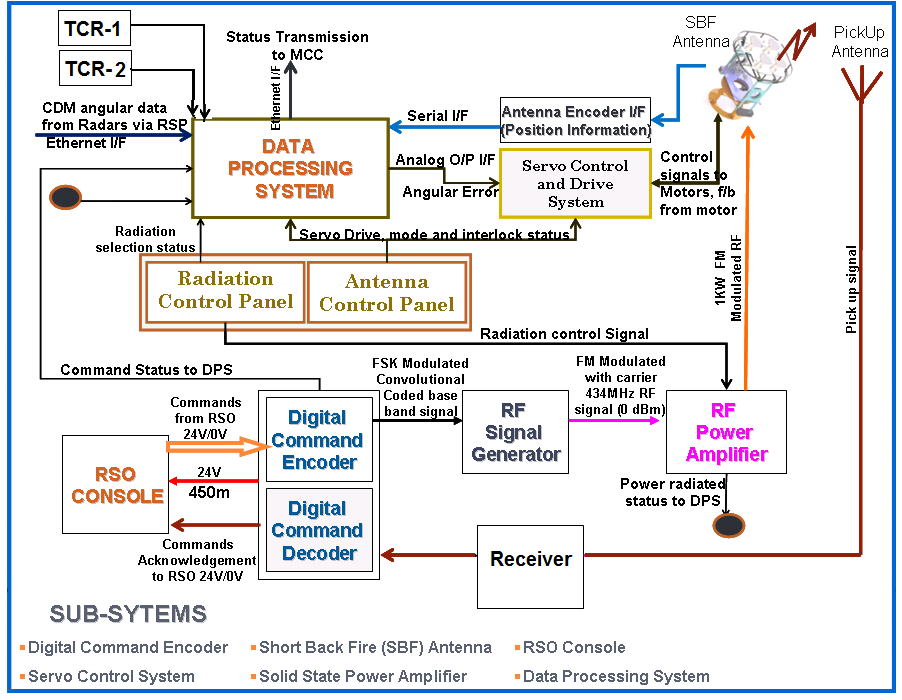
\includegraphics[width=\linewidth]{./Diagrams/TCSingleChainDiag.png}
	\caption{Single chain block diagram of Telecommand}
	\label{FIG:TcSingleChain}
\end{figure}

\begin{figure}[H]
	\centering
	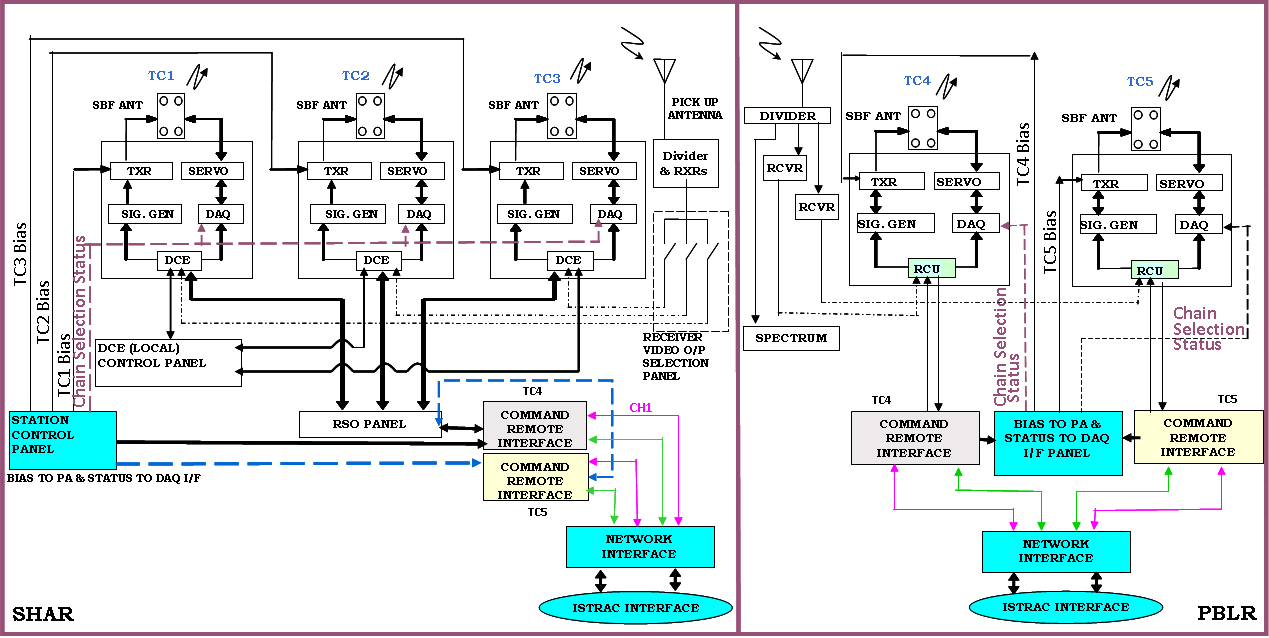
\includegraphics[width=\linewidth]{./Diagrams/TC5ChainConfg1.png}
	\caption{Five Chain Configuration of Telecommand}
	\label{FIG:FiveChConfig}
\end{figure}

\section{System Purpose}

\subsection{Data processing System}
Data Processing system is Intel Xeon 8 core processor CPU and application is designed in Qt Creator software tool on Linux platform. DPS generates error required for Azimuth and Elevation drive power amplifiers based on the present antenna positioned angle information and commanded angle information to keep the antenna orientation towards the vehicle trajectory. DPS acquires, processes, formats, packetises, displays and logs the data related to different sub-systems and the overall DPS schematic is shown in Fig. \ref{FIG:DPSSchematic}.

\begin{figure}[H]
	\centering
	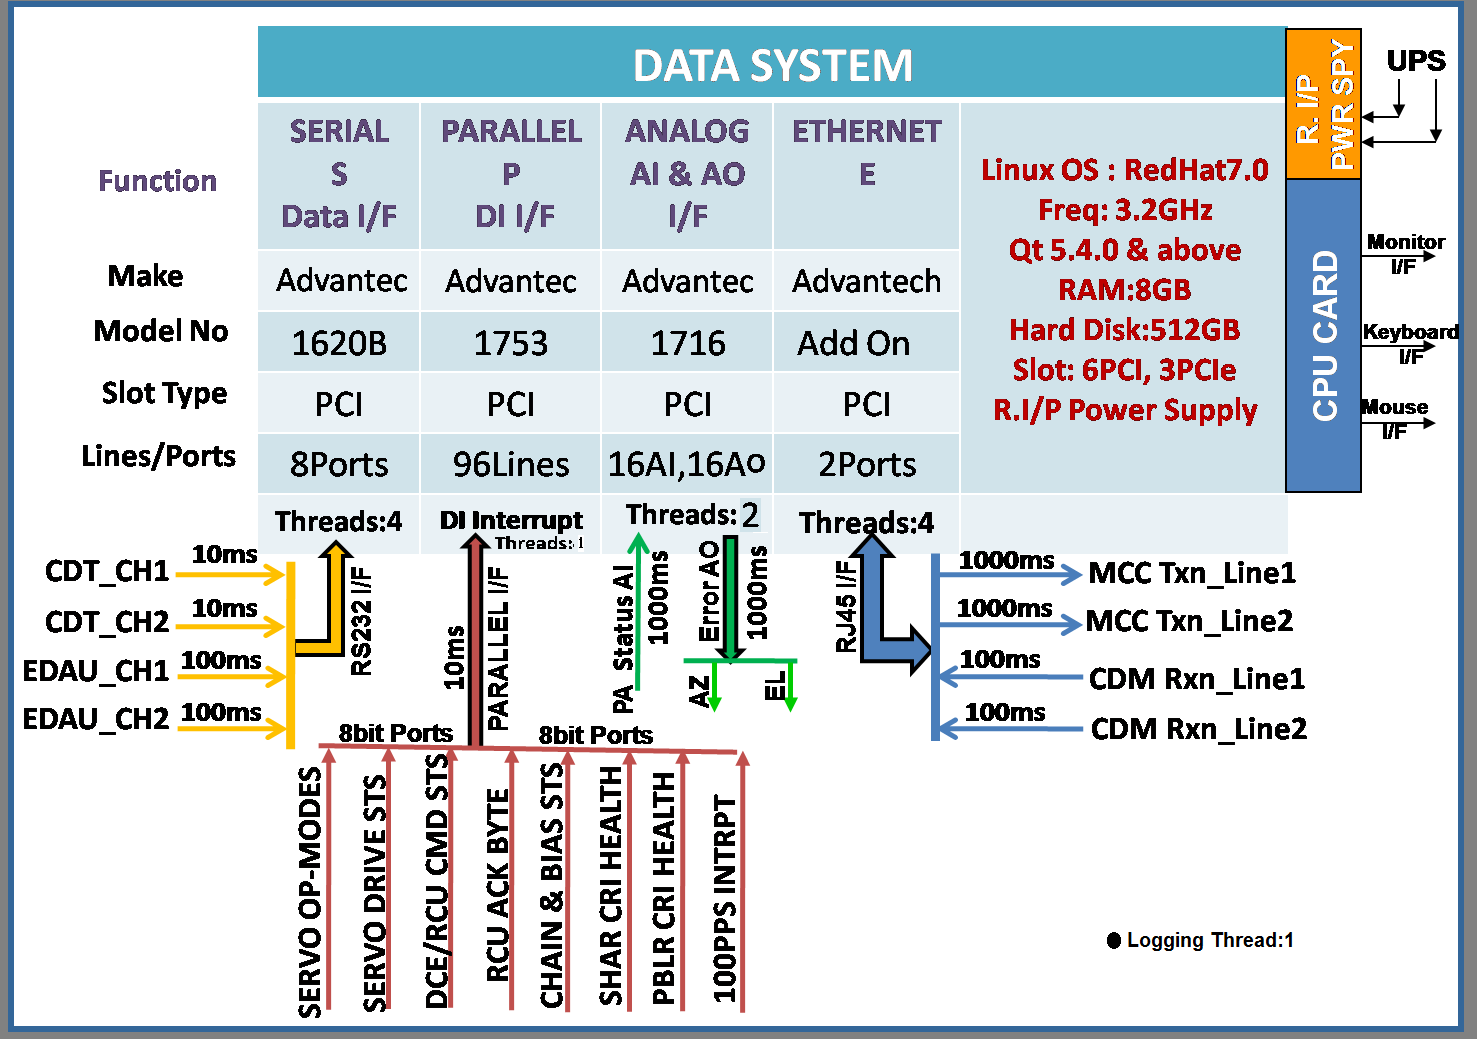
\includegraphics[width=\linewidth]{./Diagrams/DPSBlockDiagram.png}
	\caption{Overall Schematic of Data Processing System }
	\label{FIG:DPSSchematic}
\end{figure}


\subsection{Digital Command Encoder / Remote Command Unit }
Digital command encoder is based on convolution coding and decoder is based on Viterbi decoding which is implemented using FPGA board. The block level digram of DCE housed at SHAR TC is shown in Fig. \ref{FIG:DCEDiag}.The design of RCU unit positioned at PBLR is almost same as that of DCE except for the interfaces as shown in Fig. \ref{FIG:CRIConnectivity}. The system is capable of generating four commands SAFE, ARM, DESTRUCT, and COMMAND1 for vehicle command up-linking in real time.

\begin{figure}[H]
	\centering
	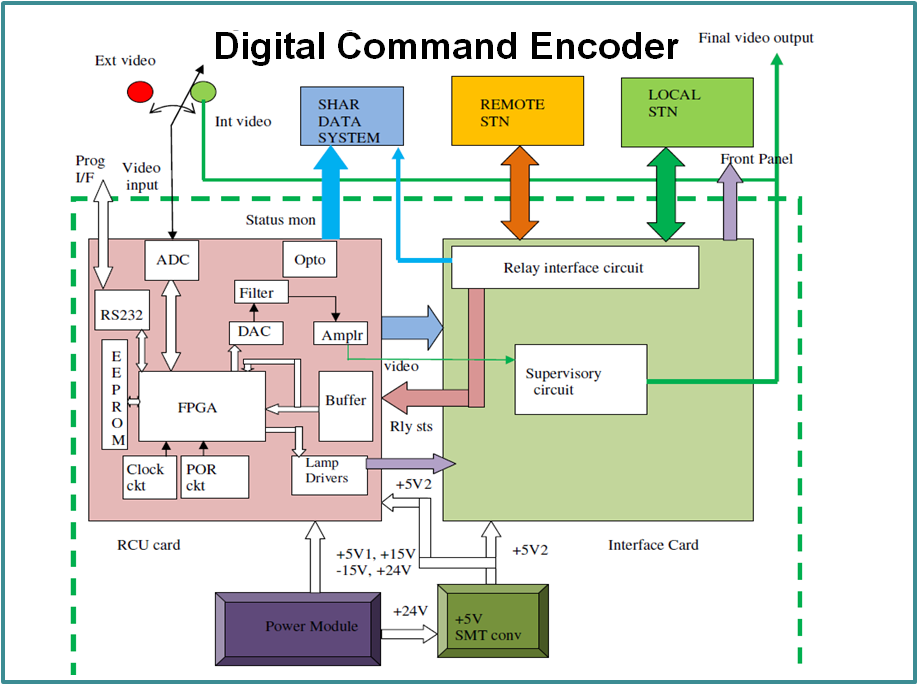
\includegraphics[width=\linewidth]{./Diagrams/DCEBlockDiag.png}
	\caption{Block Diagram of Digital Command Encoder }
	\label{FIG:DCEDiag}
\end{figure}

\subsection{Servo System}
Telecommand antenna movement is controlled using a servo system which consists of various sub systems like antenna driving motors, encoders, drive control modules, interlock logic system, operator control console, EDAU and DPS. Servo block diagram and its connectivity with other systems is shown in Fig. \ref{FIG:ServoDiag}. Antenna movement can be controlled either in open loop or closed loop. Open loop of operation includes applying joy stick deflection voltage to servo drive without involvement of DPS whereas closed loop systems includes either program mode or CDM mode for error generation using DPS and is fed to servo drive for steering the antenna.

\begin{figure}[H]
	\centering
	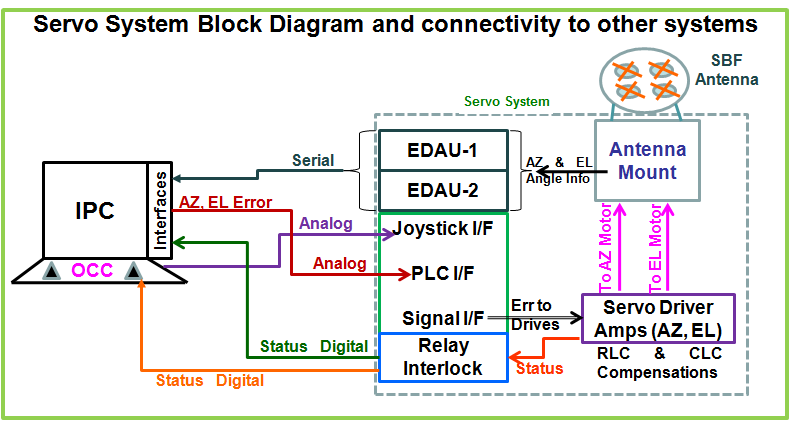
\includegraphics[width=\linewidth]{./Diagrams/BlockServo.png}
	\caption{Block Diagram of Servo System and connectivity to other systems }
	\label{FIG:ServoDiag}
\end{figure}


\subsection{Operator Control Console}
Antenna movement operations will be done from Operator Control Console. OCC consists of joysticks for manually controlling the antenna movement in open loop, operating switches and status indicators for various modes, drive power ON status, Emergency Stop operation and status indicators for pre-limit \& limit operation of antenna in both Azimuth \& Elevation axis. This is a part of servo system and is shown in Fig. \ref{FIG:ServoDiag}.

\subsection{Encoder Data Acquisition Unit}
EDAU is Microcontroller based system for acquiring, conversion from gray to binary format, converting to engineering units and displaying angular position of the antenna. It also transmits the angular information to DPS in serial format. EDAU is a part of servo systems is shown in Fig. \ref{FIG:ServoDiag}.

\subsection{Time Code Reader}
TCR provides timing information and interrupt for Telecommand DPS and 10 pps signal to EDAU unit for acquiring antenna encoder information. Single TCR provides timing information in two RS-232 ports, 10 pps \& 100 pps signals. Similar information from three TCRs is given to three TC chains at SHAR and from two TCRs is to two TC chains at PBLR in redundant cyclic manner as shown in Fig. \ref{FIG:SHARTIMINGDIST} and Fig. \ref{FIG:PBLRTIMINGDIST} respectively.

\begin{figure}[H]
	\centering
	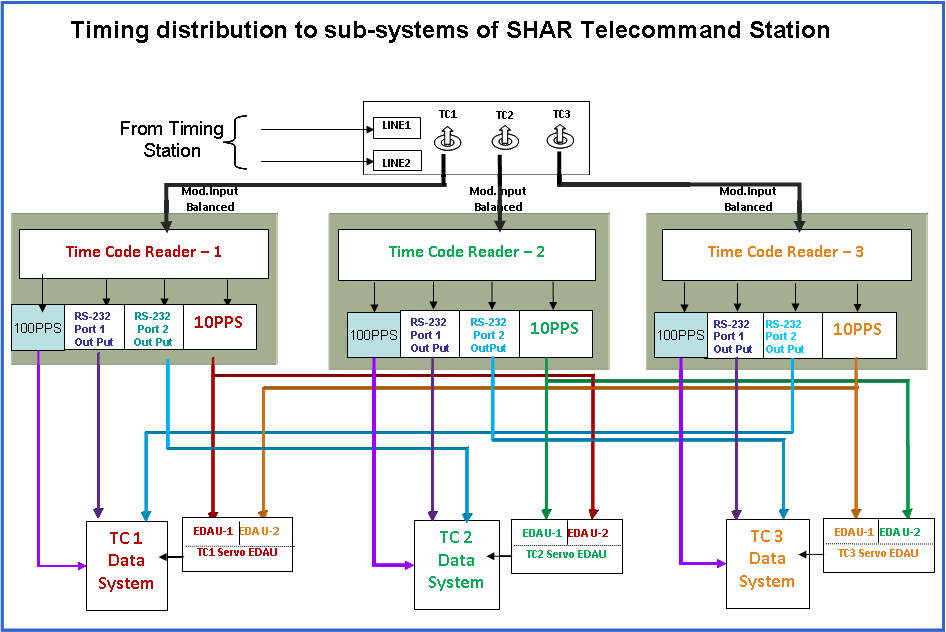
\includegraphics[width=0.9\linewidth]{./Diagrams/SharTimingDistribution.png}
	\caption{Timing distribution to sub-systems of Telecommand at SHAR}
	\label{FIG:SHARTIMINGDIST}
\end{figure}

\begin{figure}[H]
	\centering
	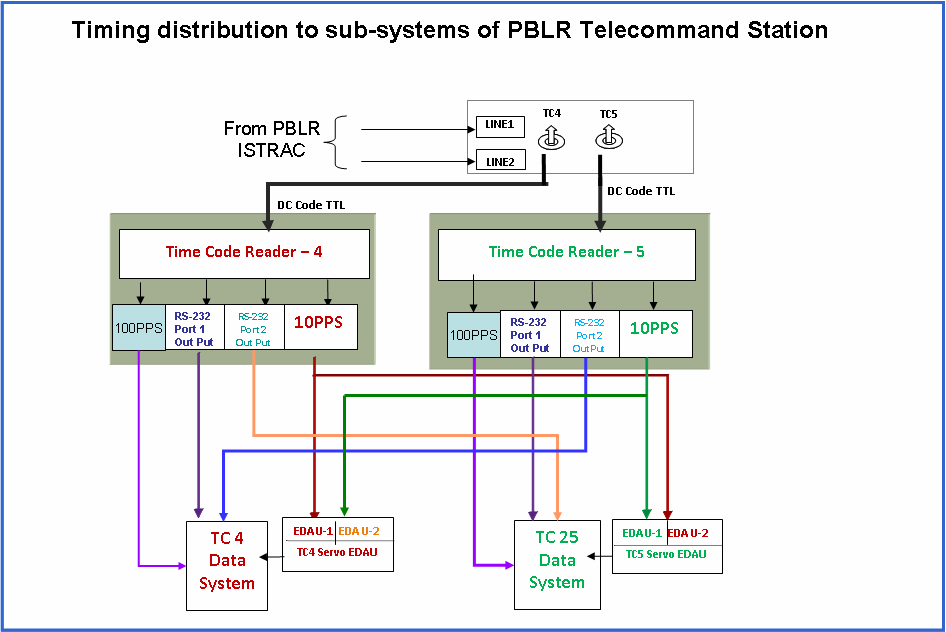
\includegraphics[width=0.9\linewidth]{./Diagrams/PBLRTimingDistribution.png}
	\caption{Timing distribution to sub-systems of Telecommand at PBLR}
	\label{FIG:PBLRTIMINGDIST}
\end{figure}


%\subsection{Integrated Telecommand Recorder}
%The command uplinked from antenna is received using a test antenna (spike/ quadra loop) and demodulated using receiver. The demodulated video output is fed back to DCE/RCU for decoding purpose. The same video output is logged using ITR at high rate (250KSps) so that actual command uplinked can be verified from logged data analysis.

\subsection{Transmitter/ Solid State Power Amplifier}
SSPA operates in the frequency band 400 to 500 MHz with a power output of 1 KW CW. Power amplifier is modular in construction, amplifies 0 dBm FM modulated RF signal to 60 dBm by employing different RF stages  and is shown in Fig. \ref{FIG:BlockPA}. ${V}_{f}$ is the DC calibrated power output and is interfaced to DPS via analog interface.

\begin{figure}[H]
	\centering
	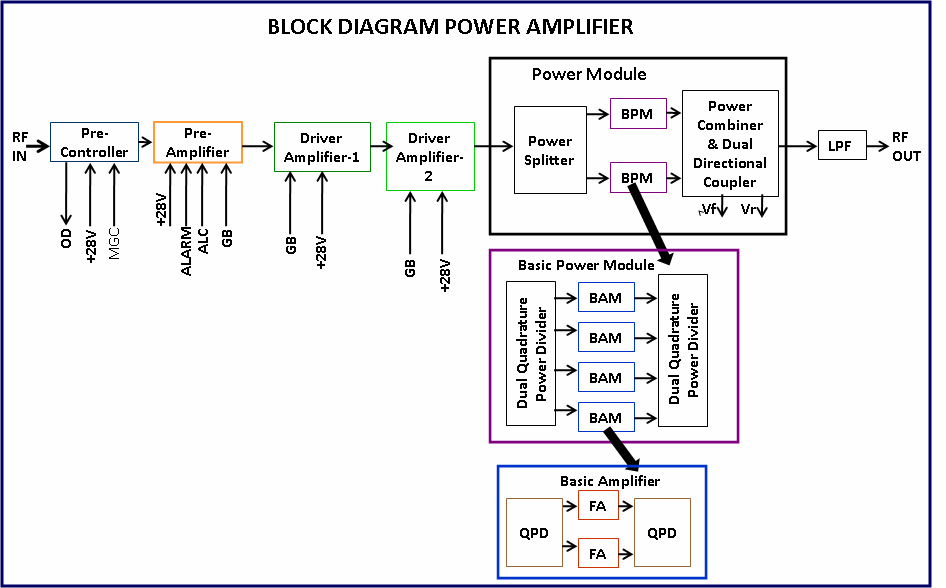
\includegraphics[width=\linewidth]{./Diagrams/BlockPA.png}
	\caption{Block Diagram of Power Amplifier}
	\label{FIG:BlockPA}
\end{figure}

\subsection{Short Back Fire Antenna}
Telecommand antenna is resonant, steerable wide beam antenna with elevation over azimuth mount. The antenna gain of 19 dBi and beam width of ${19}^{o}$ is achieved with four elements each with a gain of 13 dBi The antenna is an array of four elements each with a horizontal and vertical dipole. The antenna is called Short Back Fire antenna with RCP and the name is obtained based on its functionality. 

\subsection{Command Remote Interface}

The block level schematic of CRI showing the connectivity between RSO at SHAR with RCU at PBLR is shown in Fig. \ref{FIG:CRIConnectivity}. The CRI unit at SHAR end acquires command signal from RSO panel, Status \& control signals from SHAR TC control panel using PLC DI module.  Upon the detection of Command, the Processor will generate 2 words (2$\times$40=80 bits). Incase of SAFE or COMD1 the two words are same (Safe, Safe or comd1, comd1), whereas for DESTRUCT sequence the two words are ARM, DEST. Then these 80 bits along with source ID, bias status (radiation selection information), system in use status, CRC 16 bit polynomial check sum, packet counter, packet length are formed into 36 bytes packet and transmitted to PBLR via two ISTRAC links at 100 msec rate. \\ 

CRI at PBLR receives the packet at 100 msec rate. Change of command word will be sensed only if the three consecutive samples are same. Then, CRI transmits changed command word continuously at 100 msec rate using RS232 serial communication interface to RCU, otherwise CRI continues previous command word transmission to RCU at the same 100 msec rate. \\

CRI receives not only up-linked command status but also receives the residing command in RCU via serial RS232 interface. CRI in turn transmits the command uplinked status to RSO via ISTRAC links and command residing status to DPS via control panel.


\begin{figure}[H]
	\centering
	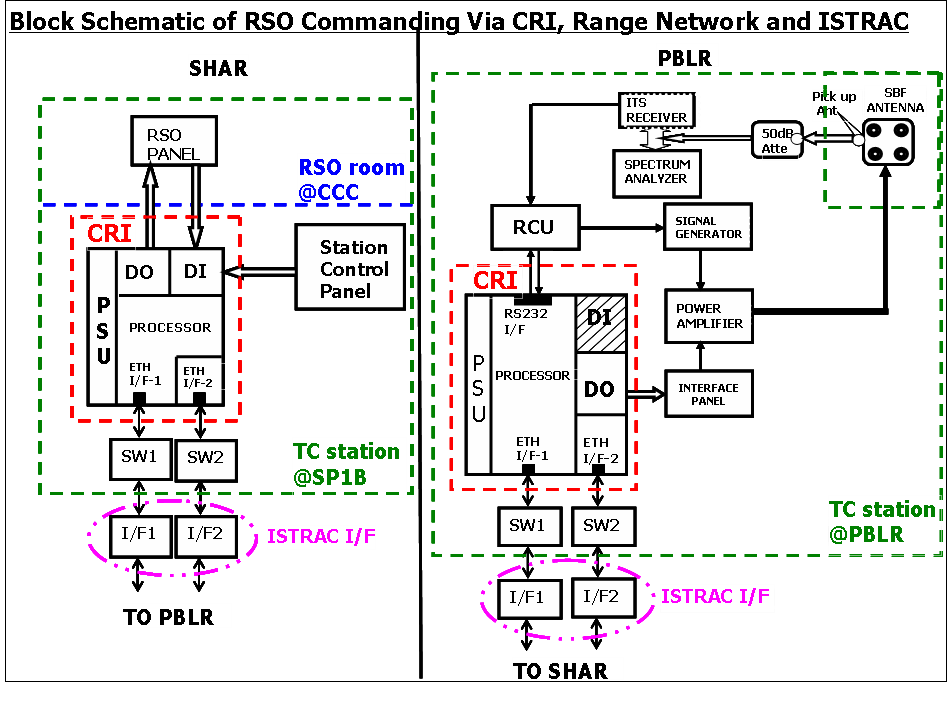
\includegraphics[width=\linewidth]{./Diagrams/BlockLevelSchematicCRISharPblr.png}
	\caption{Block level schematic of CRI connecting RSO at SHAR with RCU at PBLR}
	\label{FIG:CRIConnectivity}
\end{figure}

\section{System Scope}
The Software product named ``TC DPS" will be generated based on the Systems Requirements Specification document (SYRS) given in this document \cite{SYRSLBDPS}. Software Requirements Document (SRS) \cite{SRSLBDPS} will be generated based on SYRS and forms the base line document for software design. The industrial PC will be loaded with Red Hat Linux Enterprise version 7.0. The application will be developed in Qt Creator software tool in C++ programming language. The requirements of the TC DPS application software are mentioned in the following sections. This product does the following 

\begin{enumerate}
	\item [a)] Receives the antenna azimuth and elevation angles from the EDAU.
	\item [b)] Auto chain change over logic will be derived based on the healths of data received from EDAU chain-1 and chain-2.  
	\item [c)] Acquires the necessary inputs from the Telecommand subsystems like timing information from TCR; Status from DCE/RCU, Servo, CRI, Power Amplifier, Status Control Panel.
	\item [d)] Receives designated azimuth and elevation angles i.e., CDM data from RSP servers and processes them.
	\item [e)] Generates the necessary servo error voltages to drive the antenna so as to precisely point towards the launch vehicle in real time.
	\item [f)] The software will update the overall system status on the PC monitor display, provides Graphical User Interface (GUI).
	\item [g)] Logs the servo status, DCE parameters, EDAU parameters, station parameters, and incoming CDM data in the form of disk files.
	\item [h)] It also transmits station status parameters to MCC servers.
	
\end{enumerate}

The PCDPS, which is a part of the Telecommand system, is built around a Intel Xeon 8 core processor CPU card installed in an Industrial PC with a ${22}^{"}$ LED monitor, a keyboard, an optical mouse and redundant power supplies. The PC has a passive back plane with 6 PCI and 3 PCIe slots. These slots can accommodate the add-on cards required for the system to interact with all other subsystems of the Telecommand and the Real Time Network. 
\chapter{Decomposition description}
\label{Chapter2}
\section{Module decomposition}
\subsection{main}
\begin{enumerate}
	\item [$\blacklozenge$] To create an object for this application.
	\item [$\blacklozenge$] To initialize the settings instance for this application.	
\end{enumerate}
 
  \subsection{mainwindow}
  
  \begin{enumerate}
  	\item [$\blacklozenge$] To create the objects for the process related  classes.
  	\item [$\blacklozenge$] To read the configuration information from the input files and Network transmission.
  	\item [$\blacklozenge$] To create and begin the threads for serial i/o threads (4 nos), network reception threads (2 nos), network transmission threads (2 nos), DIO parallel (1 nos), analog input (1 nos), analog output (1 nos) and logging (1 nos).
  	\item [$\blacklozenge$] To facilitate the selection and updation of various toolbar buttons provided for user selectable functions.
  	\item [$\blacklozenge$] To start a 100 msec timer to process the acquired data periodically.
  	\item [$\blacklozenge$] To map the signals to the corresponding slots used in this class.
  	\item [$\blacklozenge$] To update the parameters for logging and parameters for plotting.
  	\item [$\blacklozenge$] To frame the data for transmission to MCC
  	\item [$\blacklozenge$] To provide display updation and graphic user interface
  		
  \end{enumerate}

    \subsection{IrigRead}
    \begin{enumerate}
    	\item [$\blacklozenge$] To read the config file "irig.txt".
    	\item [$\blacklozenge$] To Initialize the PCI variables like No.of IRIG cards ,Interrupt Rate,etc .
    \end{enumerate}
    
\section{Concurrent process decomposition}

Nil. There is only one process running at a time in this project. But there are multiple threads running. The details are as follows.
       \subsection{IrigThread} 
       
        \begin{enumerate}
       	\item [$\blacklozenge$] This is a worker thread and does not need any user interface. 
       	\item [$\blacklozenge$] This thread starts running immediately after it is created and stops only when the application is quit.  
       	\item [$\blacklozenge$] It acquires Time Data from 4 IRIG-PCI cards.
       	\item [$\blacklozenge$] The synchronization to the main thread is through signals.
       	
       \end{enumerate}	
       
       \subsection{networkTxThread} 
   
       \begin{enumerate}
    \item [$\blacklozenge$] This is a worker thread and does not need any user interface.
    \item [$\blacklozenge$] This thread starts running immediately after it is created and stops only when the application is quit.
    \item [$\blacklozenge$] This Thread Initilises the ips address of the system
   	\item [$\blacklozenge$] This Thread send the Data through Ethernet port
   
   \end{enumerate}
	
   \subsection{LogData}
      \begin{enumerate}
   	\item [$\blacklozenge$] Logs the Time data at specified rates to hard disk.
   \end{enumerate}

\section{Data decomposition}

The data entities used in this project are grouped into the following categories:
       \subsection{Input data files} 
       
        \begin{enumerate}
        \item [$\blacklozenge$] irig.txt file contains parameters for the IRIG-PCI cards. The corresponding format of this input file is given in section. \ref{section:irig_card} 
       	
       	\item [$\blacklozenge$] Tx.txt file contains configuration Tx IPs . System Ip and corresponding Port numbers The corresponding format of this input file is given in section. \ref{section:tx.} 
       	
       \end{enumerate}	
	
       \subsection{Output data files} 
       
       \begin{enumerate}
       	\item [$\blacklozenge$] Log File of Time Data 
       	. \ref{Table:tim_Log_file}
       	
       \end{enumerate}		
\chapter{Dependency description}
\label{Chapter3}
\section{Intermodule dependency}

\begin{enumerate}
	\item [$\blacklozenge$] The Intermodule dependencies are depicted in the data flow diagram and is shown in  Fig. \ref{FIG:SWDataFlowDiag}.
	\item [$\blacklozenge$] Signals and slots are used for communication between threads and 10pps interrupt handling.
	\item [$\blacklozenge$] GUI updations at 10 Hz rate and plotting updation at 1 Hz rate.
	\item [$\blacklozenge$] The details of data formats are given in section. \ref{section:LogFormats}.
\end{enumerate}

\begin{figure}[H]
	\centering
	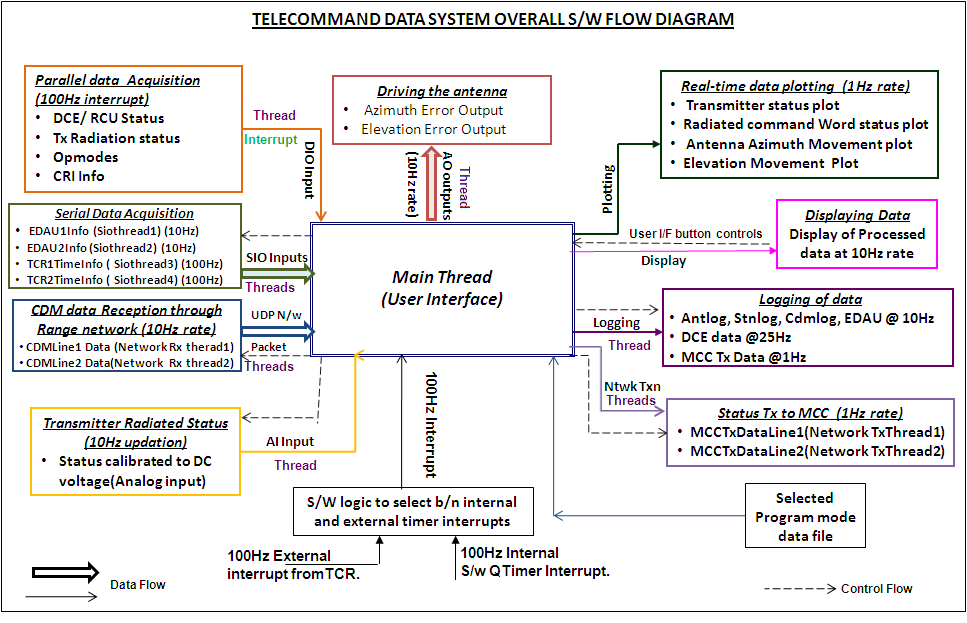
\includegraphics[width=\linewidth]{./Diagrams/SWFlowDiag.png}
	\caption{Software data flow diagram}
	\label{FIG:SWDataFlowDiag}
\end{figure}

\section{Interprocess dependencies}
Nil
\section{Data dependencies}
The data entities used in this project are grouped into the following categories:
\subsection{Input data files}
\begin{enumerate}
	
	\item [$\blacklozenge$] irig.txt file contains of the configuration parameters of IRIG-PCI cards ports for acquiring TIme data.
	\item [$\blacklozenge$] tx.txt file contains of the configuration parameters of Tx ethernet port and port numbers for acquiring data from parallel ports.
\end{enumerate}	
The details of input data configuration files are given in section. \ref{Section:InpFileFormat} and section. \ref{Section:ConnectDataPortsFormat}.

\subsection{QT  Resources}

\begin{enumerate}
	\item [$\blacklozenge$] Toolbar resource containing the buttons necessary for user interface.
	\item [$\blacklozenge$] Menubar resource containing the menu items necessary for user interface. 
	\item [$\blacklozenge$] Dialog resource for confirming selections done by the user.
	\item [$\blacklozenge$] Plotting resource for data plotting. 
	\item [$\blacklozenge$] Bitmap resource for displaying the status and updation of different parameters.
\end{enumerate}		

\subsection{System  Resources}
\begin{enumerate}
	\item [$\blacklozenge$] Memory resource.
	\item [$\blacklozenge$] Interrupt resources. 
\end{enumerate}

\subsection{Drivers}
\begin{enumerate}
	\item [$\blacklozenge$] IRIG-PCI card device drivers .
	\item [$\blacklozenge$] Qt 5.4.0 or above drivers.
	\item [$\blacklozenge$] PCI Network Ethernet drivers as a package in Red Hat Linux 7.0.
\end{enumerate}

\chapter{Interface description}
\label{Chapter4}

\section{Module Interface}
\subsection{main}
\subsection{MainWindow}
\begin{enumerate}
	\item [$\blacklozenge$] irigcard.txt (Details in section. \ref{section:tcconstants}).
	\item [$\blacklozenge$] TxSocket.txt(Details in section. \ref{section:pgm}).
	\item [$\blacklozenge$] Logdata.txt(Details in section. \ref{section:pio}).
	
\end{enumerate}

\subsection{logdata}
\begin{enumerate}
	\item [$\blacklozenge$] Logdata.txt (Details in section. \ref{section:pio}) 
\end{enumerate}

\subsection{irigRead}
\begin{enumerate}
	\item [$\blacklozenge$] irigcard.txt (Details in section. \ref{section:tcconstants}).
\end{enumerate}

\subsection{irigThread}
\begin{enumerate}
	\item [$\blacklozenge$] Nil
\end{enumerate}

\subsection{networkTxThread}
\begin{enumerate}
	\item [$\blacklozenge$] TxSocket.txt (Details in section. \ref{Label:TXSoc})
\end{enumerate}




\chapter{Detailed design}
\label{Chapter5}
\section{Module Detailed design}

\subsection{Main }
This function is created by the QT creator. It contains the QApplication object and the Mainwindow objects. This function shows the main GUI page. 
\subsubsection{Attributes}
Nil
\subsubsection{Member Functions }
Nil
\subsubsection{Slots}
Nil
\subsubsection{Signals}
Nil
\subsubsection{Internal design details }
Nil

\subsection{MainWindow}
\subsubsection{Attributes}
\begin{enumerate}
\item [$\rhd$] class NetworkTx;
\item [$\rhd$] class irig;
\item [$\rhd$] class IRIG$\_$THREAD;
\item [$\rhd$] class LogData;
\item [$\rhd$]QThread NetworkTxThread1;
\item [$\rhd$]QThread NetworkTxThread2;
\item [$\rhd$]QThread LogThread;
\item [$\rhd$]NetworkTx* m$\_$NetTx;
\item [$\rhd$] NetworkTxThread* m$\_$NetTx1;
\item [$\rhd$] NetworkTxThread* m$\_$NetTx2;
\item [$\rhd$] LogData* m$\_$DLog;
\item [$\rhd$] 
\item [$\rhd$] irig* m$\_$irig;
\item [$\rhd$] IRIG$\_$THREAD* m$\_$irig1;
\item [$\rhd$] IRIG$\_$THREAD* m$\_$irig2;
\item [$\rhd$] IRIG$\_$THREAD* m$\_$irig3;
\item [$\rhd$] IRIG$\_$THREAD* m$\_$irig4;
\item [$\rhd$] IRIG$\_$THREAD* m$\_$irig4;
\item [$\rhd$] QTimer *Timer10Hz;
\item [$\rhd$] Ui::MainWindow *ui;
\item [$\rhd$] QTimer *timer;
\item [$\rhd$] int ret;
\item [$\rhd$] int Hmsecs$\_$Count;
\item [$\rhd$] int SecondsCount;
\item [$\rhd$] quint8 LogDataFlag;
\item [$\rhd$] quint8 LogOverallFlag;
\item [$\rhd$] int irigStatus[8];

\end{enumerate}

\subsubsection{Member Functions }
\begin{enumerate}
	\item [$\blacklozenge$] void ExitOnError(void);
	\item [$\blacklozenge$] void InitializeIrigCards(void);
	\item [$\blacklozenge$] void DisScreen(void);
	\item [$\blacklozenge$] int  OpenFiles(void);
	
\end{enumerate}

\subsubsection{Slots}
\begin{enumerate}
	\item [$\blacklozenge$] void on$\_$APP$\_$EXIT$\_$clicked();
	\item [$\blacklozenge$] void on$\_$LOGenable$\_$clicked();
	\item [$\blacklozenge$] void on$\_$LOGoverall$\_$clicked();
	\item [$\blacklozenge$] void on$\_$irig1DataRxd(int NoOfBytes);
	\item [$\blacklozenge$] void on$\_$irig2DataRxd(int NoOfBytes);
	\item [$\blacklozenge$] void on$\_$irig3DataRxd(int NoOfBytes);
	\item [$\blacklozenge$] void on$\_$irig4DataRxd(int NoOfBytes);
	\item [$\blacklozenge$] void on$\_$irig4DataRxd(int NoOfBytes);
	\item [$\blacklozenge$] void TimerTicked();
	
	
\end{enumerate}

\subsubsection{Signals}
\begin{enumerate}
	\item [$\blacklozenge$] void ExitOnError(void);

	
\end{enumerate}

\subsubsection{Internal design details }
\begin{enumerate}
	\item  \textbf{MainWindow::MainWindow(QWidget *parent) :
    QMainWindow(parent),
    ui(new Ui::MainWindow)}
	\begin{enumerate}
		\item \textit{Inputs :} Nil.
		\item \textit{Functional details:} The constructor is derived from the QObject class.
		\item \textit{Outputs:} Nil.
		\item \textit{Implementation details:} In this function all IRIG threads and network threads are initilised by reading config files and made to run 
		\item \textit{File operations:} Nil.
	\end{enumerate}
	
	\item  \textbf{MainWindow::$ \sim $MainWindow()}
	\begin{enumerate}
		\item \textit{Inputs :} Nil
		\item \textit{Functional details:} 
		\item \textit{Outputs:} Nil
		\item \textit{Implementation details:} This function is Desctructor for main window class.all threads are stopped and deleted 
		\item \textit{File operations:} Nil.
	\end{enumerate}
	
	\item  \textbf{void MainWindow::ExitOnError(void)}
	\begin{enumerate}
		\item \textit{Inputs :} Nil
		\item \textit{Functional details:} This function is called to exit the program . this function exits all running thread ,delete thier instances  and also deleted all pointers to avoid memory leaks
		\item \textit{Outputs:} NIl
		\item \textit{Implementation details:} 
		\item \textit{File operations:} Nil
	\end{enumerate}
	
	\item  \textbf{int MainWindow::OpenFiles(void)}
	\begin{enumerate}
		\item \textit{Inputs :} Nil 
		\item \textit{Functional details:} 
		\item \textit{Outputs:} file opened status
		\item \textit{Implementation details:}  This function opens the config files
		\item \textit{File operations:} opens config file namely "irigcards.txt" "TxSocket".
	\end{enumerate}
	
	\item  \textbf{void MainWindow::on$\_$irig1DataRxd(int NoOfBytes)}
	\begin{enumerate}
		\item \textit{Inputs :} No of Bytes of Time code data received from card
		\item \textit{Functional details:} 
		\item \textit{Outputs:} read status 
		\item \textit{Implementation details:} This function takes the time data and logs UT-1 time
		\item \textit{File operations:} Nil
	\end{enumerate}
	
	\item  \textbf{void MainWindow::on$\_$irig2DataRxd(int NoOfBytes)}
	\begin{enumerate}
		\item \textit{Inputs :} No of Bytes of Time code data received from card
		\item \textit{Functional details:} 
		\item \textit{Outputs:} read status 
		\item \textit{Implementation details:} This function takes the time data and logs UT-2 time
		\item \textit{File operations:} Nil
	\end{enumerate}
	
	\item  \textbf{void MainWindow::on$\_$irig3DataRxd(int NoOfBytes)}
	\begin{enumerate}
		\item \textit{Inputs :} No of Bytes of Time code data received from card
		\item \textit{Functional details:} 
		\item \textit{Outputs:} read status 
		\item \textit{Implementation details:} This function takes the time data and logs CDT-1 time
		\item \textit{File operations:} Nil
	\end{enumerate}
	
	\item  \textbf{void MainWindow::on$\_$irig4DataRxd(int NoOfBytes)}
	\begin{enumerate}
		\item \textit{Inputs :} No of Bytes of Time code data received from card
		\item \textit{Functional details:} 
		\item \textit{Outputs:} read status 
		\item \textit{Implementation details:} This function takes the time data and logs CDT-2 time
		\item \textit{File operations:} Nil
	\end{enumerate}
	
	
	\item  \textbf{void MainWindow::on$\_$LOGenable$\_$clicked()}
	\begin{enumerate}
		\item \textit{Inputs :} Nil
		\item \textit{Functional details:} 
		\item \textit{Outputs:} Nil
		\item \textit{Implementation details:} This slot function called when LOG button pressed in gui.this function enables the log.
		\item \textit{File operations:} Nil
	\end{enumerate}
	
	

	
\end{enumerate}


\subsection{irig}
\subsubsection{Attributes}
\begin{enumerate}
\item [$\rhd$]struct IRIG$\_$NODE;
\item [$\rhd$]QList$<$IRIG$\_$NODE*$>$ irig$\_$list;
\item [$\rhd$] uint NoOfIrigCards;
\item [$\rhd$] uint InterruptRate;
\item [$\rhd$] int irigb$\_$size;

\end{enumerate}

\subsubsection{Member Functions }
\begin{enumerate}
	\item [$\blacklozenge$] irig::irig(QObject *parent)
	\item [$\blacklozenge$] irig::irig()
	\item [$\blacklozenge$] int irig::Read$\_$IRIG$\_$File(QString file$\_$name)
\end{enumerate}

\subsubsection{Slots}
Nil
\subsubsection{Signals}
Nil
\subsubsection{Internal design details }
\begin{enumerate}
	\item  \textbf{irig::irig(QObject *parent)}
	\begin{enumerate}
		\item \textit{Inputs :} Nil.
		\item \textit{Functional details:} The constructor is derived from the QObject class.
		\item \textit{Outputs:} Nil.
		\item \textit{Implementation details:} It is a constructor for irig class.
		\item \textit{File operations:} Nil.
	\end{enumerate}
	
	\item  \textbf{irig::irig()}
	\begin{enumerate}
		\item \textit{Inputs :} Nil
		\item \textit{Functional details:} 
		\item \textit{Outputs:} Nil
		\item \textit{Implementation details:} This function is Desctructor for irig class.
		\item \textit{File operations:} Nil.
	\end{enumerate}
	
	\item  \textbf{int irig::Read$\_$IRIG$\_$File(QString file$\_$name)}
	\begin{enumerate}
		\item \textit{Inputs :} File name of irig configuraion file //"irigcards.txt"
		\item \textit{Functional details:} 
		\item \textit{Outputs:} file read status 
		\item \textit{Implementation details:} This function reads the irigcards configuration file and initialises the irig node class.
		\item \textit{File operations:} opens "irigcards.txt" file and closes it after reading.
	\end{enumerate}
	

	
\end{enumerate}



\subsection{IRIG$\_$THREAD}
\subsubsection{Attributes}
\begin{enumerate}
	\item [$\rhd$] int fp;
	\item [$\rhd$] int fd[6]; 
	\item [$\rhd$] int NoOfCards;
	\item [$\rhd$] quint8 UT1[10],UT2[10], CDT1[10],CDT2[10],CDT3[10];
	\item [$\rhd$] int gDevNo;;
	\item [$\rhd$] int sfd[6];
	\item [$\rhd$] sigset$\_$t mask;
	\item [$\rhd$] int modevalue[8];
\end{enumerate}


\subsubsection{Member Functions }
\begin{enumerate}
	\item [$\blacklozenge$] int ConfigureIrigCard(int CardNo, QList$<$IRIG$\_$NODE*$>$ irig$\_$list, uint NoOfIrigCards,uint InterruptRate);	
	\item [$\blacklozenge$] void SelectDevice(int CardNo);
	\item [$\blacklozenge$] void run();
	\item [$\blacklozenge$] void read1();

	
\end{enumerate}
\subsubsection{Slots}
Nil


\subsubsection{Signals}
\begin{enumerate}

	\item [$\blacklozenge$] void Irig$\_$Rxd$\_$Flag(int NoOfBytes);

\end{enumerate}
\subsubsection{Internal design details }
\begin{enumerate}
	\item  \textbf{IRIG$\_$THREAD::IRIG$\_$THREAD()}
	\begin{enumerate}
		\item \textit{Inputs :} Nil.
		\item \textit{Functional details:} The constructor is derived from the QObject class.it initialises various variables in the class 
		\item \textit{Outputs:} Connects signals to slots.
		\item \textit{Implementation details:} Qt Creator 5.4, C++ language.
		\item \textit{File operations:} Nil.
	\end{enumerate}

\item  \textbf{IRIG$\_$THREAD::$\sim$ IRIG$\_$THREAD()}
\begin{enumerate}
	\item \textit{Inputs :} Nil
	\item \textit{Functional details:} This function is Destructor for the class
	\item \textit{Outputs:} Nil.
	\item \textit{Implementation details:} Qt Creator 5.4, C++ language.
	\item \textit{File operations:} Nil.
\end{enumerate}
\item  \textbf{int IRIG$\_$THREAD::ConfigureIrigCard(int CardNo,QList$<$IRIG$\_$NODE*$>$ irig$\_$list, uint NoOfIrigCards, uint InterruptRate)}
\begin{enumerate}
	\item \textit{Inputs :} Cardno, irigcard list,numofcards interruptrate
	\item \textit{Functional details:} This function opens the device and configures the device with parameters read from config file ie,"irigcard.txt"
	\item \textit{Outputs:} Nil.
	\item \textit{Implementation details:} Qt Creator 5.4, C++ language.
	\item \textit{File operations:} Opens the irig device  and writes the config parameters.
\end{enumerate}

\item  \textbf{IRIG$\_$THREAD::run()}
\begin{enumerate}
	\item \textit{Inputs :} Nil
	\item \textit{Functional details:} This function is reads the time data from device
	\item \textit{Outputs:} Nil.
	\item \textit{Implementation details:} Qt Creator 5.4, C++ language.
	\item \textit{File operations:} Opens the irig device and reads the time data to UT1,UT2,CD1,CD2 arrays.
\end{enumerate}




%\end{enumerate}


\subsection{LogData}
\subsubsection{Attributes}
\begin{enumerate}
\item [$\blacklozenge$] QString TimFileName1,TimFileName2,TimFileName3;
\item [$\blacklozenge$] QString TimFileName4,TimFileName5;
	\item [$\blacklozenge$] int TimeSamplesCount1,TimeSamplesCount2,TimeSamplesCount3
   \item [$\blacklozenge$] int 	TimeSamplesCount4,TimeSamplesCount5;
	\item [$\blacklozenge$] quint8 AppExitFlag;
	\item [$\blacklozenge$] QFile  TimFile1;
	\item [$\blacklozenge$] qint64 TimFileSize1;
	\item [$\blacklozenge$] QFile  TimFile2;
	\item [$\blacklozenge$] qint64 TimFileSize2;
	\item [$\blacklozenge$] QFile  TimFile3;
	\item [$\blacklozenge$] qint64 TimFileSize3;
	\item [$\blacklozenge$] QFile  TimFile4;
	\item [$\blacklozenge$] qint64 TimFileSize4;
	\item [$\blacklozenge$] QFile  TimFile5;
	\item [$\blacklozenge$] qint64 TimFileSize5;
\end{enumerate}
\subsubsection{Member Functions }
\begin{enumerate}
	\item [$\blacklozenge$] void GetFileName(QString Suffix);
	\item [$\blacklozenge$] void LogCode1Data(quint8 Data[]);
	\item [$\blacklozenge$] void LogCode2Data(quint8 Data[]);
	\item [$\blacklozenge$] void LogCode3Data(quint8 Data[]);
	\item [$\blacklozenge$] void LogCode4Data(quint8 Data[]);
	\item [$\blacklozenge$] void LogCode5Data(quint8 Data[]);
	\item [$\blacklozenge$] QString GetDataString(quint8 Data[], int UT$\_$CDT);
	
	
\end{enumerate}


\subsubsection{Slots}
\begin{enumerate}
	\item [$\blacklozenge$] int CopyTime1File();
	\item [$\blacklozenge$] int CopyTime2File();
	\item [$\blacklozenge$] int CopyTime3File();
	\item [$\blacklozenge$] int CopyTime4File();
	\item [$\blacklozenge$] int CopyTime5File();
	
\end{enumerate}

\subsubsection{Signals}
\begin{enumerate}
	\item [$\blacklozenge$] int TimCopyFlag1();
	\item [$\blacklozenge$] int TimCopyFlag2();
	\item [$\blacklozenge$] int TimCopyFlag3();
	\item [$\blacklozenge$] int TimCopyFlag4();
	
\end{enumerate}

\subsubsection{Internal design details }
\begin{enumerate}
	\item  \textbf{void GetFileName(QString Suffix)}
	\begin{enumerate}
		\item \textit{Inputs :} Suffix - current time in string format.
		\item \textit{Functional details:} This function reads current data time ,initilises the file name variables 
		\item \textit{Outputs:} Nil.
		\item \textit{Implementation details:} Qt Creator 5.4, C++ language.
		\item \textit{File operations:} Nil.
	\end{enumerate}
	
	\item  \textbf{QString LogData::GetDataString(quint8 Data[], int UT$\_$CDT)}
	\begin{enumerate}
		\item \textit{Inputs :} Time data in structured format.
		\item \textit{Functional details:} This function formats the time in struct to string  
		\item \textit{Outputs:} Nil.
		\item \textit{Implementation details:} Qt Creator 5.4, C++ language.
		\item \textit{File operations:} Nil.
	\end{enumerate}
	

	
	\item  \textbf{void LogData::LogCode1Data(quint8 Data[])}
	\begin{enumerate}
		\item \textit{Inputs :} Time data .
		\item \textit{Functional details:} This function insert the UT-1time data in array which will be written to disk.
		\item \textit{Outputs:} Nil.
		\item \textit{Implementation details:} Qt Creator 5.4, C++ language.
		\item \textit{File operations:} Nil.
	\end{enumerate}
	
	\item  \textbf{void LogData::LogCode2Data(quint8 Data[])}
	\begin{enumerate}
		\item \textit{Inputs :} Time data .
		\item \textit{Functional details:} This function insert the UT-2 time data in array which will be written to disk.
		\item \textit{Outputs:} Nil.
		\item \textit{Implementation details:} Qt Creator 5.4, C++ language.
		\item \textit{File operations:} Nil.
	\end{enumerate}
	
	\item  \textbf{void LogData::LogCode3Data(quint8 Data[])}
	\begin{enumerate}
		\item \textit{Inputs :} Time data .
		\item \textit{Functional details:} This function insert the CDT-1 time data in array which will be written to disk.
		\item \textit{Outputs:} Nil.
		\item \textit{Implementation details:} Qt Creator 5.4, C++ language.
		\item \textit{File operations:} Nil.
	\end{enumerate}
	
	\item  \textbf{void LogData::LogCode4Data(quint8 Data[])}
	\begin{enumerate}
		\item \textit{Inputs :} Time data .
		\item \textit{Functional details:} This function insert the CDT-2 time data in array which will be written to disk.
		\item \textit{Outputs:} Nil.
		\item \textit{Implementation details:} Qt Creator 5.4, C++ language.
		\item \textit{File operations:} Nil.
	\end{enumerate}
	
	\item  \textbf{void LogData::LogCode5Data(quint8 Data[])}
	\begin{enumerate}
		\item \textit{Inputs :} Time data .
		\item \textit{Functional details:} This function insert the time data in array which will be written to disk.
		\item \textit{Outputs:} Nil.
		\item \textit{Implementation details:} Qt Creator 5.4, C++ language.
		\item \textit{File operations:} Nil.
	\end{enumerate}
	
	
	\item  \textbf{int LogData::CopyTime1File()}
	\begin{enumerate}
		\item \textit{Inputs :} Nil .
		\item \textit{Functional details:} This Slot function which will be called on emission of signal TimCopyFlag1,it will write the array of time samples to disk.
		\item \textit{Outputs:} Nil.
		\item \textit{Implementation details:} Qt Creator 5.4, C++ language.
		\item \textit{File operations:} Nil.
	\end{enumerate}
	
	\item  \textbf{int LogData::CopyTime2File()}
	\begin{enumerate}
		\item \textit{Inputs :} Nil .
		\item \textit{Functional details:} This Slot function which will be called on emission of signal TimCopyFlag1.it will write the array of time samples to disk.
		\item \textit{Outputs:} Nil.
		\item \textit{Implementation details:} Qt Creator 5.4, C++ language.
		\item \textit{File operations:} Nil.
	\end{enumerate}
	
	\item  \textbf{int LogData::CopyTime3File()}
	\begin{enumerate}
		\item \textit{Inputs :} Nil .
		\item \textit{Functional details:} This Slot function which will be called on emission of signal TimCopyFlag1,it will write the array of time samples to disk.
		\item \textit{Outputs:} Nil.
		\item \textit{Implementation details:} Qt Creator 5.4, C++ language.
		\item \textit{File operations:} Nil.
	\end{enumerate}
	\item  \textbf{int LogData::CopyTime4File()}
	\begin{enumerate}
		\item \textit{Inputs :} Nil .
		\item \textit{Functional details:} This Slot function which will be called on emission of signal TimCopyFlag1.it will write the array of time samples to disk.
		\item \textit{Outputs:} Nil.
		\item \textit{Implementation details:} Qt Creator 5.4, C++ language.
		\item \textit{File operations:} Nil.
	\end{enumerate}
	
\end{enumerate}


\subsection{NetworkTx}


\subsubsection{Attributes}
\begin{enumerate}
	\item [$\rhd$] QByteArray datagram;;
	\item [$\rhd$] int socketEnable;
	\item [$\rhd$] int Socket;
	
	\item [$\rhd$] QHostAddress ForeignHost;
	
	
	\item [$\rhd$] int ForeignPort;
	
	\item [$\rhd$] unsigned long int MCCserTxCount;
	\item [$\rhd$] unsigned long int MCCserErrCount;
	\item [$\rhd$] quint8 SerTxFlag;
	\item [$\rhd$] int NoOf$\_$TxSockets;
	
	
\end{enumerate}
\subsubsection{Member Functions }
\begin{enumerate}
	\item [$\blacklozenge$] int NetworkTxInit(int socketNo, QList$<$TXSOCKETNODE*$>$ net$\_$TxList, int NoOfTxSockets);
\end{enumerate}

\subsubsection{Slots}
\begin{enumerate}
	\item [$\blacklozenge$] void sendDatagram(QByteArray datagram);
\end{enumerate}
\subsubsection{Signals}
\begin{enumerate}
	\item [$\blacklozenge$] void netTxdFlag(QByteArray sup$\_$sys$\_$data);
\end{enumerate}

\subsubsection{Internal design details }
\begin{enumerate}
	\item  \textbf{ int NetworkTxInit(int socketNo, QList<TXSOCKETNODE*> net$\_$TxList, int NoOfTxSockets)}
	\begin{enumerate}
		\item \textit{Inputs :} Socket no, list of socket interfaces ,No of sockets
		\item \textit{Functional details:} This function intilises the network interface accoding to the config file "TxSocket.txt"
		\item \textit{Outputs:} Nil.
		\item \textit{Implementation details:} Nil.
		\item \textit{File operations:} Nil.
	\end{enumerate}

\item  \textbf{void sendDatagram(QByteArray datagram)}
\begin{enumerate}
	\item \textit{Inputs :} Time packet data in QByte array format.
	\item \textit{Functional details:} Sends the Ethernet packet 
	\item \textit{Outputs:} Nil.
	\item \textit{Implementation details:} Nil.
	\item \textit{File operations:} Nil.
\end{enumerate}
\end{enumerate}


\subsection{Network Reception: NetworkRx} 

This class is derived from the QObject class. It is instantiated in the MainWindow class.
\subsubsection{Attributes}
\begin{enumerate}
	\item [$\rhd$] int NoOfRxSockets
	\item [$\rhd$] QList$<$RXSOCKETNODE*$>$ net$\_$RxList
	\item [$\rhd$] int messageNo
\end{enumerate}

\subsubsection{Member Functions }
\begin{enumerate}
	\item [$\blacklozenge$] int ReadNetworkRxFile(QString file$\_$name)
\end{enumerate}


\subsubsection{Slots}
Nil

\subsubsection{Signals}
Nil


\subsubsection{Internal design details }
\begin{enumerate}
	\item  \textbf{NetworkRx::NetworkRx()}
	\begin{enumerate}
		\item \textit{Inputs :} Nil.
		\item \textit{Functional details:} The constructor is derived from the QThread class.
		\item \textit{Outputs:} Network Thread class generated.
		\item \textit{Implementation details:} Nil.
		\item \textit{File operations:} Nil.
	\end{enumerate}
	\item  \textbf{NetworkRx :: ReadNetworkRxFile(char* file$\_$name)}
	\begin{enumerate}
		\item \textit{Inputs :} Configuration file name.
		\item \textit{Functional details:} The configuration file containing the number of sockets and the network configuration parameters for each socket is opened and read. A linked list containing the configuration details of each socket is created.
		\item \textit{Outputs:} Socket configuration details read and stored. 
		\item \textit{Implementation details:} QT Linux 5.4 calls are used to implement this function.
		\item \textit{File operations:} UdpRxSocket.inp
	\end{enumerate}   
\end{enumerate}

\subsection{Network Transmission: NetworkTx}

\subsubsection{Attributes}
\begin{enumerate}
	\item [$\rhd$] int NoOfTxSockets
	\item [$\rhd$] QList$<$TXSOCKETNODE*$>$ net$\_$TxList
\end{enumerate}

\subsubsection{Member Functions }
\begin{enumerate}
	\item [$\blacklozenge$] int ReadNetworkTxFile(QString file$\_$name)
	\end{enumerate}


\subsubsection{Slots}
Nil

\subsubsection{Signals}
Nil

\subsubsection{Internal design details }
\begin{enumerate}
	\item  \textbf{NetworkRx :: ReadNetworkTxFile(QString file$\_$name)}
	\begin{enumerate}
		\item \textit{Inputs:} Configuration file name
		\item \textit{Functional details:} The configuration file containing the number of sockets and the network configuration parameters for each socket is opened and read. A linked list containing the configuration details of each socket is created.
		\item \textit{Outputs:} Socket configuration details read and stored. 
		\item \textit{Implementation details:} QT Linux 5.4 calls are used to implement this function.
		\item \textit{File operations:} UdpTxSocket.inp
	\end{enumerate}  
\end{enumerate}


\section{Threads detailed design}

\subsection{Network Reception Thread: NetworkRxThread} \label{NtWkRxThd}
\begin{enumerate}
	\item [$\rhd$] This is a worker thread and does not need any user interface.
	\item [$\rhd$] This thread starts running immediately after it is created and stops when the application is quit.
	\item [$\rhd$] It acquires UDP/IP packets in UNICAST mode i.e., receives CDM data.
	\item [$\rhd$] Data to be received from two sockets.
	\item [$\rhd$] The synchronization to the main thread is through signals.
\end{enumerate}
This class is derived from the QThread class. It is instantiated and started in the MainWindow class.
\subsubsection{Attributes}
\begin{enumerate}
	\item [$\rhd$] QUdpSocket *udpRxSocket
	\item [$\rhd$] int messageNo
	\item [$\rhd$] QByteArray RxSocketData
	\item [$\rhd$] bool NetworkRxInit(int,QList$<$RXSOCKETNODE*$>$)
	\item [$\rhd$] quint8 rxsocketno
	\item [$\rhd$] bool NetRx$\_$OK$\_$flag
	\item [$\rhd$] quint64 nopacketreceptioncount$\_$L1;
	\item [$\rhd$] quint64 nopacketreceptioncount$\_$L2;
	\item [$\rhd$] uint Line1packetSize;
	\item [$\rhd$] uint Line2packetSize;
\end{enumerate}

\subsubsection{Member Functions }
\begin{enumerate}
	\item [$\blacklozenge$] bool NetworkRxInit(int,QList $<$RXSOCKETNODE*$>$)
\end{enumerate}


\subsubsection{Slots}
\begin{enumerate}
	\item [$\blacklozenge$] void readPendingDatagrams()
	\item [$\blacklozenge$] void closesocket()
\end{enumerate}

\subsubsection{Signals}
\begin{enumerate}
	\item [$\blacklozenge$] void Line1CDMDataRxd(int,QByteArray)
	\item [$\blacklozenge$] void Line2CDMDataRxd(int,QByteArray)
\end{enumerate}


\subsubsection{Internal design details }
\begin{enumerate}
	\item  \textbf{NetworkRxThread::NetworkRxThread()}
	\begin{enumerate}
		\item \textit{Inputs :} Nil.
		\item \textit{Functional details:} The constructor is derived from the QThread class.
		\item \textit{Outputs:} Network Thread class generated.
		\item \textit{Implementation details:} Nil.
		\item \textit{File operations:} Nil.
	\end{enumerate}
	
	\item  \textbf{NetworkRxThread :: NetworkRxInit()}
	\begin{enumerate}
		\item \textit{Inputs :} Nil.
		\item \textit{Functional details:} The required number of UDP sockets are created and configured as per the details read and stored. A slot is identified to service the readyread signal generated on reception of data.
		\item \textit{Outputs:} Sockets are configured. 
		\item \textit{Implementation details:} QT Linux 5.4 calls are used to implement this function.
		\item \textit{File operations:} Nil.
	\end{enumerate}
	\item \textbf{NetworkRxThread :: readPendingDatagrams()}
	\begin{enumerate}
		\item \textit{Inputs :} Readyread signal.
		\item \textit{Functional details:} On the occurrence of readyread signal, the socket which raised the signal is identified and the corresponding data is copied to a QByteArray variable. A signal is then raised to the Mainwindow indicating the reception of new CDM data frame along with the socket number (1 or 2).
		\item \textit{Outputs:} CDM data is received.
		\item \textit{Implementation details:} QT Linux 5.4 calls are used to implement this function.
		\item \textit{File operations:} Nil.
	\end{enumerate}   
\end{enumerate}





\subsection{Network Transmission Threads: NetworkTx }

\subsubsection{Attributes}
\begin{enumerate}
	\item [$\rhd$] NetrxMc$\_$Txn datagram
	\item [$\rhd$] QByteArray mcc$\_$Tx$\_$Buf2
	\item [$\rhd$] QByteArray mcc$\_$Tx$\_$Buf1
	\item [$\rhd$] quint64 line2$\_$MCC$\_$Cnt
	\item [$\rhd$] quint64 line1$\_$MCC$\_$Cnt	
	\item [$\rhd$] QUdpSocket *udpTxSocket
	\item [$\rhd$] int messageNo
	\item [$\rhd$] QByteArray RxSocketData
	\item [$\rhd$] bool NetTx$\_$OK$\_$flag
	\item [$\rhd$] quint64 line1$\_$No$\_$Tx$\_$Count
	\item [$\rhd$] quint64 line2$\_$No$\_$Tx$\_$Count	
\end{enumerate}

\subsubsection{Member Functions }
\begin{enumerate}
	\item [$\blacklozenge$] void NetworkTxInit()
\end{enumerate}


\subsubsection{Slots}
\begin{enumerate}
	\item [$\blacklozenge$] void sendDatagram1(QByteArray ,int,quint8)
	\item [$\blacklozenge$] void sendDatagram2(QByteArray ,int,quint8)
\end{enumerate}

\subsubsection{Signals}
\begin{enumerate}
	\item [$\blacklozenge$] void SignalForTx2MCC(QByteArray ,int,quint8 )
\end{enumerate}

\subsubsection{Internal design details }
\begin{enumerate}
	\item  \textbf{NetworkRx :: NetworkTxInit()}
	\begin{enumerate}
		\item \textit{Inputs:} Nil.
		\item \textit{Functional details:} Nil.
		\item \textit{Outputs:} Nil. 
		\item \textit{Implementation details:} Nil.
		\item \textit{File operations:} Nil.
	\end{enumerate}
	\item \textbf{NetworkRx :: sendDatagrams1(QByteArray mcc$\_$buf$\_$Txn,  int i, quint8 Tx$\_$Packetsize)}
	\begin{enumerate}
		\item \textit{Inputs :} Byte array to be transmitted, line number, packet size to be transmitted, 
		\item \textit{Functional details:}  writeDatagram writes data on to the socket-1 and returns number of bytes transmitted if successful, else -1 will be returned. 
		\item \textit{Outputs:} Writes data on to the socket-1 for transmission.
		\item \textit{Implementation details:} QT Linux 5.4 calls are used to implement this function.
		\item \textit{File operations:} Nil.
	\end{enumerate}  
	\item \textbf{NetworkRx :: sendDatagrams2(QByteArray mcc$\_$buf$\_$Txn,  int i, quint8 Tx$\_$Packetsize)}
	\begin{enumerate}
	\item \textit{Inputs :} Byte array to be transmitted, line number, packet size to be transmitted, 
	\item \textit{Functional details:}  writeDatagram writes data on to the socket-2 and returns number of bytes transmitted if successful, else -1 will be returned. 
	\item \textit{Outputs:} Writes data on to the socket-2 for transmission.
	\item \textit{Implementation details:} QT Linux 5.4 calls are used to implement this function.
	\item \textit{File operations:} Nil.
	\end{enumerate}  
\end{enumerate}


%************************************
\subsection{siothreads: SioThread, SioThreadE}



\subsubsection{Attributes}

\textbf{SioThread : For CDT and EDAU}\\
\begin{enumerate}
	\item [$\rhd$] QSerialPort *serial	
	\item [$\rhd$] QByteArray sio$\_$data
	\item [$\rhd$] quint8 SIO$\_$Status
	\item [$\rhd$] qint64 Total$\_$Bytes
	\item [$\rhd$] quint8 sio1$\_$ret
	\item [$\rhd$] quint8 sioPort
	\item [$\rhd$] bool serialclear
	\item [$\rhd$] bool sio$\_$OK$\_$ststus$\_$flag
	\item [$\rhd$] quint64 data1normalcount
	\item [$\rhd$] quint64 data2normalcount
	\item [$\rhd$] quint64 data1absentcount
	\item [$\rhd$] quint64 data2absentcount
	\item [$\rhd$] uint Rxd1Bytes
	\item [$\rhd$] uint Rxd2Bytes
\end{enumerate}

\subsubsection{Member Functions } 
\begin{enumerate}
	\item [$\rhd$] Sio()
	\item [$\rhd$] int Read$\_$Sio$\_$File(QString file$\_$name)
\end{enumerate}
\textbf{SioThread : For CDT and EDAU}\\
\begin{enumerate}
	\item [$\blacklozenge$] int ConfigureSioCard(int i, QList$<$SIO$\_$Node*$>$ sio$\_$list, qint64 TotalBytes)
\end{enumerate}
\subsubsection{Slots}
\textbf{SioThread : For CDT and EDAU}\\
\begin{enumerate}
	\item [$\blacklozenge$] void readData1()
\end{enumerate}
\begin{enumerate}
	\item [$\blacklozenge$] void readData2()
\end{enumerate}

\subsubsection{Signals}
\textbf{SioThread : For CDT and EDAU}\\
\begin{enumerate}
	\item [$\blacklozenge$] void CDT1$\_$recvd(int,QByteArray)
	\item [$\blacklozenge$]void CDT2$\_$recvd(int,QByteArray)
	\item [$\blacklozenge$] void EDAU1$\_$recvd(int,QByteArray)
	\item [$\blacklozenge$]void EDAU2$\_$recvd(int,QByteArray)
\end{enumerate}

\subsubsection{Internal design details }
\begin{enumerate}
	\item  \textbf{Sio :: Sio()}
	\begin{enumerate}
		\item \textit{Inputs :} Nil.
		\item \textit{Functional details:} Objects of type QSerialPort are instantiated for 8 serial ports.
		\item \textit{Outputs:} 8 serial port objects are created.
		\item \textit{Implementation details:} 	QT Linux 5.4 libraries are used to implement the above.
		\item \textit{File operations:} Nil.
	\end{enumerate}
	
	\item  \textbf{Sio :: Read$\_$Sio$\_$File(QString file$\_$name)}
	\begin{enumerate}
		\item \textit{Inputs :} Configuration input file name.
		\item \textit{Functional details:} The number of serial ports and the corresponding configuration details are read and a linked list of serial port details is generated. 
		\item \textit{Outputs:} Serial port configuration details read and stored.
		\item \textit{Implementation details:} QT Linux 5.4 libraries are used to implement the above.
		\item \textit{File operations:} sio.txt.
	\end{enumerate}
	
	\item  \textbf{SioThread :: int ConfigureSioCard(int i, QList$<$SIO$\_$Node*$>$ sio$\_$list, qint64 TotalBytes)}
	\begin{enumerate}
		\item \textit{Inputs :} Serial port number, total bytes, serial linked list.
		\item \textit{Functional details:} The required number of serial ports are as per the details stored in the linked list. 
		\item \textit{Outputs:} Serial ports configured. 
		\item \textit{Implementation details:} QT Linux 5.4 libraries are used to implement the above.
		\item \textit{File operations:} Nil.
	\end{enumerate}

\end{enumerate}

\section{Data detailed design}

\subsection{Data structures}
\subsubsection{CDT}
\begin{enumerate}
	\item quint8 units$\_$10Hz 
	\item quint8 sign       
	\item quint8 lift$\_$off  
	\item quint8 hmsec    
	\item quint8 sec       
	\item quint8 min        
	\item quint8 hrs        
	\item quint8 hold
\end{enumerate}
\subsubsection{Constants}
\begin{enumerate}
	\item int tc$\_$chain;   
	\item float azenc$\_$wild$\_$sample$\_$tolerance;
	\item float elenc$\_$wild$\_$sample$\_$tolerance;
	\item float enc1$\_$az$\_$bias;
	\item float enc1$\_$el$\_$bias;
	\item float enc2$\_$az$\_$bias;
	\item float enc2$\_$el$\_$bias;
	\item float az$\_$cdm$\_$slope;
	\item float az$\_$prog$\_$slope;
	\item float el$\_$cdm$\_$slope;
	\item float el$\_$prog$\_$slope;
	\item int analog$\_$channel$\_$no; 
	\item float PA$\_$Upperlimit;
	\item float PA$\_$lowerlimit;
	\item QString prog$\_$file1;
	\item uint DIO$\_$PortNo$\_$ServoOpModes;
	\item uint DIO$\_$PortNo$\_$ServoDrive$\_$RCU3Bits;
	\item uint DIO$\_$PortNo$\_$DCERCUStatus;
	\item uint DIO$\_$PortNo$\_$TxBiasSys;
	\item uint DIO$\_$PortNo$\_$CRIPBLRHealth;
	\item uint DIO$\_$PortNo$\_$CRISHARHealth;
	\item uint DIO$\_$NoOf$\_$Ports;
	\item float Az$\_$UpperLimit;
	\item float Az$\_$LowerLimit;
	\item float El$\_$UpperLimit;
	\item float El$\_$lowerLimit;
	\item int Dio$\_$Devicenumber;
	\item qint32 Dio$\_$Item;
	\item qint32 Ai$\_$Devicenumber;
	\item qint32 An$\_$Item;
	\item quint8 LogCnterDelay;
	\item QString logfolder;	
\end{enumerate}

\subsubsection{AntLog}
\begin{enumerate}
	\item quint64 ProcessCount
	\item qint64 Line1$\_$EHMS
	\item qint64 Line2$\_$EHMS
	\item qint64 Selected$\_$EHMS
	\item int CDT$\_$SelectedLine
	\item char ext$\_$int
	\item uint Az$\_$DriveOn$\_$TcProcess
	\item uint El$\_$DriveOn$\_$TcProcess
	\item uint EmStop$\_$TcProcess
	\item uint Az$\_$OpMode$\_$TcProcess
	\item uint El$\_$OpMode$\_$TcProcess
	\item float Commanded$\_$Az$\_$El$\_$TcProcess[2]
	\item float AntennaPosition$\_$Az$\_$El$\_$TcProcess[2]
	\item float Error$\_$Az$\_$El$\_$TcProcess[2]
	\item float Az$\_$ch1
	\item float El$\_$ch1
	\item float Az$\_$ch2
	\item float El$\_$ch2
	\item bool EDAUCurrentChainSelectedFlag
	\item bool EDAUCh1$\_$OverallHealth
	\item bool EDAUCh2$\_$OverallHealth
	\item bool EDAUCh1$\_$IntExtStatusforProc
	\item bool EDAUCh2$\_$IntExtStatusforProc
	\item int CDM$\_$SelectedLine
	\item int CDM$\_$SelectedSource
	\item float Az$\_$CDM1$\_$Src1
	\item float El$\_$CDM1$\_$Src1
	\item float Az$\_$CDM1$\_$Src2
	\item float El$\_$CDM1$\_$Src2
	\item float Az$\_$CDM2$\_$Src1
	\item float El$\_$CDM2$\_$Src1
	\item float Az$\_$CDM2$\_$Src2
	\item float El$\_$CDM2$\_$Src2
	\item uint ID$\_$CDM1$\_$Src1
	\item uint ID$\_$CDM1$\_$Src2
	\item uint ID$\_$CDM2$\_$Src1
	\item uint ID$\_$CDM2$\_$Src2
	\item uint CompFlag$\_$CDM1
	\item uint CompFlag$\_$CDM2
	\item quint64 cdm1$\_$RxCount
	\item quint64 cdm2$\_$RxCount
	\item quint64 Pres$\_$cdm$\_$L1$\_$Src1$\_$Count
	\item quint64 Pres$\_$cdm$\_$L1$\_$Src2$\_$Count
	\item quint64 Pres$\_$cdm$\_$L2$\_$Src1$\_$Count
	\item quint64 Pres$\_$cdm$\_$L2$\_$Src2$\_$Count
	\item quint64 line1$\_$MCC$\_$Cnt
	\item quint64 line2$\_$MCC$\_$Cnt
	\item bool Antlog$\_$Selection$\_$Flag
	\item quint64 AntlogCounter
\end{enumerate}

\subsubsection{Acquired$\_$encoder$\_$Data}
\begin{enumerate}
	\item qint64 Line1$\_$EHMS
	\item qint64 Line2$\_$EHMS
	\item qint64 Selected$\_$EHMS
	\item int EDAUChain1$\_$id
	\item float Az$\_$hnds$\_$ch1
	\item float Az$\_$tens$\_$ch1
	\item float Az$\_$ones$\_$ch1
	\item float Az$\_$1tenth$\_$ch1
	\item float Az$\_$1hundredth$\_$ch1
	\item float El$\_$hnds$\_$ch1
	\item float El$\_$tens$\_$ch1
	\item float El$\_$ones$\_$ch1
	\item float El$\_$1tenth$\_$ch1
	\item float El$\_$1hundredth$\_$ch1
	\item char Edau1$\_$ExtIntLog
	\item int EDAUchain1$\_$HealthByte
	\item int EDAUChain1$\_$EndByte
	\item float Az$\_$ch1
	\item float El$\_$ch1
	\item int EDAUChain2$\_$id
	\item float Az$\_$hnds$\_$ch2
	\item float Az$\_$tens$\_$ch2
	\item float Az$\_$ones$\_$ch2
	\item float Az$\_$1tenth$\_$ch2
	\item float Az$\_$1hundredth$\_$ch2
	\item float El$\_$hnds$\_$ch2
	\item float El$\_$tens$\_$ch2
	\item float El$\_$ones$\_$ch2
	\item float El$\_$1tenth$\_$ch2
	\item float El$\_$1hundredth$\_$ch2
	\item char Edau2$\_$ExtIntLog
	\item int EDAUchain2$\_$HealthByte
	\item int EDAUChain2$\_$EndByte
	\item float Az$\_$ch2
	\item float El$\_$ch2
	\item bool EDAUCh1$\_$OverallHealth
	\item bool EDAUCh2$\_$OverallHealth
	\item quint32 EDAUCh1$\_$NotHelathCnt
	\item quint32 EDAUCh2$\_$NotHelathCnt
	\item quint32 EDAUCh1$\_$Data$\_$NotProcessedCnt
	\item quint32 EDAUCh2$\_$Data$\_$NotProcessedCnt
	\item bool EDAUCh1$\_$IntExtStatusforProc
	\item bool EDAUCh2$\_$IntExtStatusforProc
	\item bool EDAUCurrentChainSelectedFlag
	\item float EDAUDataforProc$\_$Az
	\item float EDAUDataforProc$\_$El
	\item bool EDAUCh1 InitialisedFlag
	\item bool EDAUCh2 InitialisedFlag
	\item bool EDAUCh1 JumpsFlag
	\item bool EDAUCh2 JumpsFlag
	\item quint64 EDAUCh1 WildSampleCnt
	\item quint64 EDAUCh2 WildSampleCnt
\end{enumerate}

\subsubsection{NetRxMc}
\begin{enumerate}
	\item quint32 range1
	\item quint32   azimuth1
	\item quint32 elevation1 
	\item quint32 radartime
	\item quint32 cdm$\_$source1
	\item quint32 range2 
	\item quint32 azimuth2
	\item quint32 elevation2 
	\item quint32 rangetime
	\item quint32 cdm$\_$source2 
	\item quint32 sys$\_$id
	\item quint32 comp$\_$flags
\end{enumerate}

\subsubsection{Stnlog}
\begin{enumerate}
	\item uint station$\_$Id
	\item uint system$\_$In$\_$use
	\item quint64 ProcessCount
	\item qint64 Line1$\_$EHMS
	\item qint64 Line2$\_$EHMS
	\item qint64 Selected$\_$EHMS
	\item char ext$\_$int
	\item bool TcReadyNotReady$\_$TcProcess
	\item bool TcRadiateNotRadiate$\_$TcProcess
	\item uint PowerStatus
	\item float powerLevel
	\item bool DCE$\_$RCU$\_$Health$\_$TcProcess
	\item bool DCE$\_$RCU$\_$ComdControl$\_$TcProcess
	\item uint DCE$\_$RCU$\_$ComdWord$\_$TcProcess
	\item quint64 cdm1$\_$RxCount
	\item quint64 cdm2$\_$RxCount
	\item quint64 Pres$\_$cdm$\_$L1$\_$Src1$\_$Count
	\item quint64 Pres$\_$cdm$\_$L1$\_$Src2$\_$Count
	\item quint64 Pres$\_$cdm$\_$L2$\_$Src1$\_$Count
	\item quint64 Pres$\_$cdm$\_$L2$\_$Src2$\_$Count
	\item quint64 line1$\_$MCC$\_$Cnt
	\item quint64 line2$\_$MCC$\_$Cnt
	\item quint8 CRI$\_$SHAR$\_$Health$\_$Processor$\_$TcProcess
	\item quint8 CRI$\_$SHAR$\_$Health$\_$Eth1$\_$TcProcess
	\item quint8 CRI$\_$SHAR$\_$Health$\_$Eth2$\_$TcProcess
	\item quint8 CRI$\_$SHAR$\_$Health$\_$DI$\_$TcProcess
	\item quint8 CRI$\_$SHAR$\_$Health$\_$DO$\_$TcProcess
	\item quint8 CRI$\_$SHAR$\_$Health$\_$RUN$\_$TcProcess
	\item bool CRI$\_$PBLR$\_$Health$\_$Processor$\_$TcProcess
	\item bool CRI$\_$PBLR$\_$Health$\_$Eth1$\_$TcProcess
	\item bool CRI$\_$PBLR$\_$Health$\_$Eth2$\_$TcProcess
	\item bool CRI$\_$PBLR$\_$Health$\_$DI$\_$TcProcess
	\item bool CRI$\_$PBLR$\_$Health$\_$DO$\_$TcProcess
	\item bool CRI$\_$PBLR$\_$Health$\_$RUN$\_$TcProcess
	\item quint8 RCU$\_$3Bit$\_$Status$\_$TcProcess
	\item bool Stnlog$\_$Selection$\_$Flag
	\item bool Dio$\_$OkStatus$\_$flag
	\item quint64 AO$\_$WriteSuccessCount
	\item quint64 AO$\_$WriteErrorCount
	\item quint64 Sio1$\_$datanormalcount
	\item quint64 Sio1$\_$dataabsentcount
	\item quint64 Sio2$\_$datanormalcount
	\item quint64 Sio2$\_$dataabsentcount
	\item quint64 Sio3$\_$datanormalcount
	\item quint64 Sio3$\_$dataabsentcount
	\item quint64 Sio4$\_$datanormalcount
	\item quint64 Sio4$\_$dataabsentcount
	\item quint64 nopacketRxCount$\_$L1
	\item quint64 nopacketRxCount$\_$L2
	\item quint64 StnlogCounter
\end{enumerate}

\subsubsection{DCE$\_$RCUlog}
\begin{enumerate}
	\item char Ch1$\_$sign      
	\item quint8 Ch1$\_$hrs        
	\item quint8 Ch1$\_$min        
	\item quint8 Ch1$\_$sec      
	\item quint8 Ch1$\_$hmsec    
	\item char Ch2$\_$sign      
	\item quint8 Ch2$\_$hrs        
	\item quint8 Ch2$\_$min       
	\item quint8 Ch2$\_$sec       
	\item quint8 Ch2$\_$hmsec    
	\item quint8 DCE$\_$RCU$\_$ComdWord
	\item bool DCE$\_$RCU$\_$Health
	\item bool DCE$\_$RCU$\_$LocalRemote
	\item bool SynthesisedPowerHealth
\end{enumerate}

\subsubsection{NetTxMCC}
\begin{enumerate}
	\item quint8 stationid
	\item quint8 chainid
	\item quint8 tcchainsts
	\item quint8 comdencsts
	\item quint8 txpwrsts
	\item quint8 servosts
	\item quint8 azcdmlsb
	\item quint8 azcdmmsb
	\item quint8 azposlsb
	\item quint8 azposmsb
	\item quint8 azerrlsb
	\item quint8 azerrmsb
	\item quint8 elcdmlsb
	\item quint8 elcdmmsb
	\item quint8  elposlsb
	\item quint8  elposmsb
	\item quint8 encochaininfo
	\item quint8 cdtsec
	\item quint8 cdtmin
	\item quint8 cdthrs
	\item quint8 cdt$\_$hmsec
	\item quint8 elerrlsb
	\item quint8 elerrmsb
	\item quint8 block$\_$id$\_$msb
	\item quint8 block$\_$id$\_$lsb
	\item quint8 tx$\_$PLC$\_$Status$\_$SHAR
	\item quint8 tx$\_$PLC$\_$Status$\_$PBLR
	\item quint8 tx$\_$PLC$\_$Status$\_$SHAR$\_$RCU$\_$3Bit
	\item quint64 Mcc$\_$Txline$\_$count
                  
\end{enumerate}

\subsubsection{cdm1$\_$buffer}
\begin{enumerate}
	\item quint8quint64 ProcessCount
\item qint64 Line1$\_$EHMS
\item qint64 Line2$\_$EHMS
\item qint64 Selected$\_$EHMS
\item char ext$\_$int
\item int range1
\item int azimuth1
\item int elevation1
\item int Radartime
\item int cdm$\_$source1
\item int range2
\item int azimuth2
\item int elevation2
\item int Rangetime
\item int cdm$\_$source2
\item int sys$\_$id
\item int comp$\_$flag
\item quint8 packetsize
\item quint64 cdm1$\_$RxCount
\item quint64 Pres$\_$cdm$\_$L1$\_$Src1$\_$Count
\item quint64 Pres$\_$cdm$\_$L1$\_$Src2$\_$Count
\item quint64 Cdm1logCounter
\end{enumerate}

\subsubsection{cdm2$\_$buffer}
\begin{enumerate}
	\item quint8quint64 ProcessCount
	\item qint64 Line1$\_$EHMS
	\item qint64 Line2$\_$EHMS
	\item qint64 Selected$\_$EHMS
	\item char ext$\_$int
	\item int range1
	\item int azimuth1
	\item int elevation1
	\item int Radartime
	\item int cdm$\_$source1
	\item int range2
	\item int azimuth2
	\item int elevation2
	\item int Rangetime
	\item int cdm$\_$source2
	\item int sys$\_$id
	\item int comp$\_$flag
	\item quint8 packetsize
	\item quint64 cdm2$\_$RxCount
	\item quint64 Pres$\_$cdm$\_$L2$\_$Src1$\_$Count
	\item quint64 Pres$\_$cdm$\_$L2$\_$Src2$\_$Count
	\item quint64 Cdm2logCounter
\end{enumerate}

\subsection{Input data files}

The details of input files are given in section. \ref{Section:InpFileFormat} and the corresponding pin/port assignments along with formats are given in section. \ref{Section:ConnectDataPortsFormat}.

\subsection{Configuration files}
The details of input configuration files are given in section. \ref{Section:InpFileFormat} and the corresponding pin/port assignments along with formats are given in section. \ref{Section:ConnectDataPortsFormat}.
 
\chapter{Procedure for loading Linux Operating System and other drivers along with add on cards}
\label{Chapter6}

\section{Loading of Redhat Linux Operating System} 

\begin{enumerate}
	\item [\textbullet] Insert RHEL7 DVD
	\item [\textbullet] Press delete/enter : it will go to boot means
	\item [\textbullet] Here select : $\#$option(with SSTA DVD) for boot priorities. Then Save $\&$ exit (files)
	\item [\textbullet] DVD
	\item [\textbullet] It will ask for time $\&$ date, software sections.
	\item [\textbullet] In the software selection, go to server with GUI option. In the following six points select required tools or packages.
		\begin{enumerate}
			\item [a)] Compatibility libraries
			\item [b)] Java
			\item [c)] KDE
			\item [d)] Hardware priorities
			\item [e)] Performance tools
			\item [f)] Development tools
		\end{enumerate}
	\item [\textbullet] Then go for Automatic partition selection. Here make sure that 114.5 GB free space is available. If not, make it free using windows vista OS CD/DVD or any windows OS CD/DVD. Then use the following partitions.
		\begin{enumerate}
			\item [a)] \textit{Boot :} /boot 512 MB
			\item [b)] \textit{Root :} / 50 MB
			\item [c)] \textit{User :} /user 10 GB
			\item [d)] \textit{Var :} /var 10 GB
			\item [e)] \textit{Home :} home 20 GB
			\item [f)] \textit{Swap :} swap 1 GB (aproximately double the ram size 8 GB)
		\end{enumerate}
	\item [\textbullet] Begin for Installation
	\item [\textbullet] Set Root password as telecommand123 and user along with password  as given below \\
			$username	: telecommand$ \\
			$password	: telecommand$
	\item [\textbullet] After completion and installation of loading of OS, reboot the system.
	\item [\textbullet] Accept the license and finish the configuration.		
\end{enumerate}

\section{Copying packages and repository creation}
\subsection{Copying of packages}

\begin{enumerate}
	\item [\textbullet] Go to $\#$home  
	\item [\textbullet] Create a folder and name it as ``mserver". \\ This will be a local server file. Instead of mounting RHEL7 DVD everytime, one can use this folder.
	\item [\textbullet] Inside ``mserver" folder, create another folder and name it as ``RHEL7". In this ``RHEL7" folder, copy all the available files in packages folder in CD/DVD  (total of 4300 files to be copied).
\end{enumerate}

\subsection{Repository creation}
All the packages are copied and the packages are available in the path ``/home/mserver/RHEL7"

\begin{enumerate}
	\item [\textbullet] First go the folder ``RHEL7" where all the packages are available. 
	\item [\textbullet] Open DVD, go to repodata, then copy ``...comps.xml" file to packages/RHEL7
	\item [\textbullet] Go to path /home/mserver (where, earlier all packages are copied), paste ``...comps.xml" and re-name to ``comps.xml" 
	\item [\textbullet] Go to the path /home/mserver
			\begin{enumerate}
				\item [a)] Go to root\\
				$\#$su\\
				$\#$pw: telecommand123 (if different, enter root password)
				\item [b)] $\#$ createrepo -g RHEL7/comps.xml\\
				repository will be created
				\item [c)] $\#$ vi /etc /yum repos.d/rhel7.repo \\
				editing the file in vi edit tool\\
				$[rhel7]$\\
				name=rhel7\\
				baseurl=file:///home/tc/mserver (where tc is user name, if user name for the pc is telecommand then in place of tc, telecommand to be written)\\
				enabled =1\\
				gpgcheck=0\\		
				Here for editing, i: insert; press with esc then :wq	
				\item [d)] $\#$ yum repolist all\\
				to know all the available repositories.
				\item [e)] $\#$ yum makecache
				\item [f)] $\#$ yum install kernel $~$devel gcc $\&$$\&$ yum update
			\end{enumerate}
\end{enumerate}

\section{Installation of libraries}

\begin{enumerate}
	\item [\textbullet] Go to the packages where all are available (/home/mserver/rhel7).
	\item [\textbullet] The execute the following files. Execute the file by double clicking. It will ask for dependencies and authentication. Enter root password and give install. The the file will be installed, otherwise ``file is already installed" message will come. Search for the following files in search bar.
	\begin{enumerate}
		\item [a)] libattr -2.4 (2 files)
		\item [b)] libattr -devel (2 files)
		\item [c)] lib coll (2 files))
		\item [d)] libcap -2.22 (2 files)
		\item [e)] libcap -devel (2 files)
		\item [f)] libavc -136u (2 files)
		\item [g)] mesa -libGLU -9.0.0
		\item [h)] mesa libGL -devel
	\end{enumerate}
	\item [\textbullet] gcc, gcc+ libraries
		\begin{enumerate}
			\item [a)] $\#$yum install libmpc.i686
			\item [b)] $\#$yum install libcap-ng-devel.i686
			\item [c)] $\#$yum install libcgroup.i686
			\item [d)] $\#$yum install libattrgroup.i686
			\item [e)] $\#$libcgroup -0.41.6....
			\item [f)] $\#$libcroco -0.6.8.5...
			\item [g)] $\#$libcxgb3 
		\end{enumerate}
\end{enumerate}	


\section{Installation of Qt}
\begin{enumerate}
	\item [\textbullet] Copy qt enterprise linux X64-5.4.0 and Qt licence in /home folder
	\item [\textbullet] Make the file as executable.\\ Go to properties.\\
	Go to permissions.\\
	Tick/select for allow as executable file. \\
	Then go to root and do the following
		\begin{enumerate}
			\item [a)] $\#$su  (go to root via terminal)
			\item [b)] $\#$pw (enter root password) 
			\item [c)] $\#$ls (to get the list of files)
			\item [d)] $\#$ ./qt-enterprise-linux-x64-5.4.0.run 
			\item [e)] Installation wizard will appear. Go tick for enter manual install details option and proceed.
				\begin{enumerate}
					\item License : XXXXUserXXXX
					\item QtLey	: XXXXKeyXXXX
					\item QtLey	: XXXXKeyXXXX \\
					copy key ``XXXXKeyXXXX" from license file.
				\end{enumerate}
		\end{enumerate}
	\item [\textbullet] Select all tools under qt.5.4.0 for installation.
	\item [\textbullet] Installation will go to the folder /opt/qt5.4 in root account (if already there, go to root and delete the file).
	\item [\textbullet] Go step by step and agree license tems and conditions.
	\item [\textbullet] Finish installation.
	\item [\textbullet] Restart the system.
\end{enumerate}

\section{Installation of drivers for add-on cards}
Copy AddonDrivers in /home folder
\subsection{blacklisting}
	\begin{enumerate}
		\item [\textbullet] Go to terminal and then to root (su and then root password)
		\item [\textbullet] $\#$yum makecache
		\item [\textbullet] $\#$yum install kernel-devel gcc $\&$$\&$ yum update kernel\\
		if already done, then this can be ignored. 
		\item [\textbullet] $\#$ vi /etc/modprobe.d/blacklist.conf
		\begin{enumerate}
			\item blacklist comedi
			\item blacklist $adv\_pci\_dio$ 
			\item blacklist $adv\_pci1710$ 
		\end{enumerate}
	These three lines are to be added using `i' for inserting and `esc+shift :wq' for saving.
	\end{enumerate}
\subsection{Adding several ports to system}
To add several ports to the system, go to root via terminal (su and root password) and do the following\\
$\#$sudo usermod -a -G dialout tc\\
where `tc' is the user of the system to be verified. If the user name is `telecommand', then `telecommand' to be used in place of `tc'.
\subsection{Serial Card installation : PCI1620B}
\begin{enumerate}
	\item [\textbullet] Go to V3.39 (in AddonDrivers folder which is located in /home)
	\item [\textbullet] Then go to `Src' which contains either a or b.
		\begin{enumerate}
			\item [a)] $adv950\_source_v3.39.tar.gz$ a zipped file. \\ For un-zipping: in this location go to terminal \& root, then un-zipping can be done using the following command in terminal\\
			$\#$ tar -xzvf $adv950\_source_v3.39.tar.gz$ \\
			It creates: $adv950\_source_v3.39$ 
			\item [b)] If already contains, un-zipped file then no need of un-zipping again
		\end{enumerate}
	\item [\textbullet] Go to the folder: $adv950\_source_v3.39$, \\
	$\#$ ls\\
	gives: 2.4  2.6  3.x advmknod get config readme
	\item [\textbullet] In this go to the folder `3.x'
	\item [\textbullet] In this folder, open terminal and root
	\item [\textbullet] $\#$make
	\item [\textbullet] $\#$depmod
	\item [\textbullet] Completes serial card installation
	\item [\textbullet] Restart the PC
	\item [\textbullet] After re-starting, check for the availability of serial ports using the following 
		\begin{enumerate}
			\item \textbf{For Comports information}: $\#$ setserial -g /dev/ttyS*
			\item \textbf{For Moxa ports information}:
			$\#$ setserial -g /dev/ttyAP*
		\end{enumerate}
\end{enumerate}

\subsection{DIO Parallel Card installation : PCI1753}
\begin{enumerate}
	\item [\textbullet] Go to AddonDrivers folder
	\item [\textbullet] Go to $Linuxdriver\_Source$ \textbf{(i)}
	\item [\textbullet] Go to drivers
	\item [\textbullet] Go to $driver\_base$
	\item [\textbullet] Go to src
	\item [\textbullet] Go to $lnx\_ko$ \\
	here open terminal in root. 
		\begin{enumerate}
			\item $\#$ make\\
			exit from here.
		\end{enumerate}
	\item [\textbullet] Go back to folder `drivers'\\
		$lnx\_ko$ $\Rightarrow$ src $\Rightarrow$ $driver\_base$ $\Rightarrow$ drivers\\
		now we are in `drivers' folder
	\item [\textbullet] Go to $pci1753\_mic3753_pcm3753i$ 
	\item [\textbullet] Go to src
	\item [\textbullet] Go to $lnx\_ko$ \\
	here open terminal in root
		\begin{enumerate}
			\item $\#$ make
			\item $\#$ mkdir /lib/modules/ \textdollar (uname -r)/biodaq \\
		exit from here.
		\end{enumerate}
	\item [\textbullet] Go back to `drivers' folder again\\
	Now we are in drivers folder\\
	Open terminal in root
		\begin{enumerate}
			\item $\#$ cp bin/*.ko /lib/modules/\textdollar (uname -r)/biodaq/
			\item $\#$ depmod
			\item $\#$ vi /etc/modules-load.d/biodaq.conf //
			Type the following three lines using `i' for inserting and `esc+shift :wq' for saving. \\
			$\#$Load biodaq at boot\\
			biokernbase\\
			bio1753\\
			exit from here.
		\end{enumerate}
	\item [\textbullet] Go back to \textbf{(i)}, i.e., outside of drivers folder and into $Linuxdriver\_Source$
	\item [\textbullet] Go to libs\\
	Now we are in libs folder \\
	Here open terminal in root \\
	\begin{enumerate}
		\item $\#$ cp * /usr/lib \\
		Exit from here
	\end{enumerate}
	\item [\textbullet] Go back to \textbf{(i)}, i.e., outside of drivers folder and into $Linuxdriver\_Source$
	\item [\textbullet] Go to inc folder \\
	Now we are in `inc' folder \\
	Here open terminal in root 
		\begin{enumerate}
			\item $\#$ cp bdaqctrl.h /usr/include/
			\item $\#$ mkdir /usr/share/Advantech
			\item $\#$ cp Automation.BDaq.jar /usr/share/Advantech/
			\item $\#$ chmod 444 /usr/share/Advantech/Automation.BDaq.jar \\
			Exit from here
		\end{enumerate}
	\item [\textbullet] This completes PCi1753 DIO drivers installation
	\item [\textbullet] Restart the system
	\item [\textbullet] After re-starting, check for the availability of daq devices using the following 
	\begin{enumerate}
		\item \textbf{To get number of daq devices}: Go to root,  $\#$ ls /dev/daq* \\
		For example, if it is displayed like the following\\
		/dev/daq0             /dev/daq255   : It means that two devices are there.
		\item \textbf{To get description of particular daq}:
		$\#$ cat /sys/class/daq/daq0/desc   : It gives description of daq0 device.
	\end{enumerate}
	
\end{enumerate}

\subsection{Multifunction Card installation : PCI1716}
Already DIO card PCI1753 installation is successful. Then with minimal installation PCI1716 installation can be done as given below
\begin{enumerate}
	\item [\textbullet] Go to AddonDrivers folder
	\item [\textbullet] Go to $Linuxdriver\_Source$ 
	\item [\textbullet] Go to PCI1716 folder
	\item [\textbullet] Go to SRC
	\item [\textbullet] Go to $lnx\_ko$ \\
	here open terminal in root. 
		\begin{enumerate}
			\item $\#$ make
			\item $\#$ depmod
			\item $\#$ vi/etc/$modules\_load.d$/biodaq.conf\\
			From the above points after entering this, we will get the following window because already during `PCI1753' the file was edited and saved.
			\begin{enumerate}
				\item load biodaq at boot
				\item biokernbase
				\item bio1753
			\end{enumerate}
			The above three points already used at devise PCI1753 
			\begin{enumerate}
				\item bio1716 \textbf{(newly entered)}\\
				 to be added using `i' for inserting and `esc+shift :wq' for saving.\\
				 Exit from here.
			\end{enumerate}	 
		\end{enumerate}
\end{enumerate}

\section{Other useful Commands}

\begin{enumerate}
	\item [\textbullet] $\#$ cntr+L				: to clear
	\item [\textbullet] $\#$ systemctl reboot	: to reboot
	\item [\textbullet] $\#$ ls /dev/daq*		: to get list of daq devices
	\item [\textbullet] $\#$ cat /sys/class/daq/daq0/desc					: to get details of paticular daq for example] daq0		
	\item [\textbullet] $\#$ lsmod		: to get list of modules
	\item [\textbullet] $\#$ free -m	: to get ram details
	\item [\textbullet] $\#$ fdisk -l	: to know the partition information
	\item [\textbullet] $\#$ cat /proc/cpuinfo : to get processor information
	\item [\textbullet] $\#$ lspci	: to get list of PCI devices
	\item [\textbullet] $\#$ minicom -s : to open communication terminal for serial port testing
	\item [\textbullet] $\#$ setserial -g /dev/ttyS*	 : to get details of serial ports in the PC
	\item [\textbullet] $\#$ su	: to enter to root user
	\item [\textbullet] $\#$ gcc -o targetExeFileName cfileName	: to compile, buid and output executable file.
	\item [\textbullet] $\#$ systemctl status firewall.d	: to know about firewall active status.
	\item [\textbullet] $\#$ systemctl status iptables	: to know about iptables active status.
	\item [\textbullet] $\#$ top: in root mode gives the memory along with cpu usage.
	\item [\textbullet] $\#$ vmstat : in root mode gives virtual memory status
	\item [\textbullet] $\#$ chmod 777 filename : in root mode assigns full writing and reading control for the file.
	\item [\textbullet] $\#$ goto root (su and then root password) cd /var/log; then to see messages give `vim messages' or `gedit messages'
	\item [\textbullet] $\#$ ifconfig : to get Ethernet configurations details.
	
	
	
	
\end{enumerate}
\chapter{Data Formats}
\label{Chapter7}
\section{RS-232 Pin assignment details}
The details of 9pin d-type connector for 8 ports of serial communication used in PCI-1620B moxa serial card are
	\begin{enumerate}
		\item [$\rhd$] Pin-1: Data clear
		\item [$\rhd$] Pin-2: Reception
		\item [$\rhd$] Pin-3: Transmission
		\item [$\rhd$] Pin-4: Data Send Ready
		\item [$\rhd$] Pin-5: Ground
		\item [$\rhd$] Pin-6: Data Terminal Ready
		\item [$\rhd$] Pin-7: Clear To Send
		\item [$\rhd$] Pin-8: Request To Send
		\item [$\rhd$] Pin-9: NC
	\end{enumerate}
\textbf{Note:} For loop back testing the following pins are to be shorted so that whatever is transmitted can be received and verified.
\begin{enumerate}
	\item [i)] Pin-1, Pin-4, Pin-6 are to be shorted
	\item [ii)] Pin-2, Pin-3 are to be shorted
	\item [iii)] Pin-7, Pin-8 are to be shorted
\end{enumerate}
\section{Input File formats}
\label{Section:InpFileFormat}

\subsection{Input file: ``tcconstants.inp" format} \label{section:tcconstants}
This is a constants file where user can define the following parameters. These parameters are used for programmable limits/values for the following TC chain information, wild sample tolerance for azimuth as well as elevation, bias for azimuth and elevation of both encoder chains, slope values for CDM and PROG mode errors, analog channel number to which power amplifier level is extended, limits of power levels, trajectory file information, DIO port numbers for statuses of servo, DCE/RCU, chain selection with chain readiness information, software limits for azimuth and elevation in either directions, device numbers and item numbers for DIO and AI cards, plotting interval, folder to which data can be saved.
\begin{table}[H]
	\centering
	
%	\caption{Constants}
	\label{Table:Constants}
	\resizebox{420pt}{300pt}{
		\caption{Constants}
		\begin{tabular}{|l|l|l|l|}
			\hline
			\textbf{S.No} & \textbf{Data variable}           & \textbf{Data type} & \textbf{Description}                                                                                                        \\ \hline
			1             & tc\_chain                        & unsignedchar       & telecommandChain no.                                                                                                        \\ \hline
			2             & az\_enc\_wild\_sample\_tolerance & float              & \begin{tabular}[c]{@{}l@{}}Azimuth Encoder Wild\\ sample rejection tolerance\end{tabular}                                   \\ \hline
			3             & el\_enc\_wild\_sample\_tolerance & float              & \begin{tabular}[c]{@{}l@{}}Elevation Encoder Wild\\ sample rejection tolerance\end{tabular}                                 \\ \hline
			4             & enc1\_az\_bias                   & float              & Encoder1 Azimuth Bias                                                                                                       \\ \hline
			5             & enc1\_el\_bias                   & float              & Encoder1 Elevation Bias                                                                                                     \\ \hline
			6             & enc2\_az\_bias                   & float              & Encoder2 Azimuth Bias                                                                                                       \\ \hline
			7             & enc2\_el\_bias                   & float              & Encoder2 Elevation Bias                                                                                                     \\ \hline
			8             & az\_cdm\_slope                   & float              & Azimuth CDM Mode Slope                                                                                                      \\ \hline
			9             & az\_prog\_slope                  & float              & Azimuth Program mode slope                                                                                                  \\ \hline
			10            & el\_cdm\_slope                   & float              & Elevation CDM Mode Slope                                                                                                    \\ \hline
			11            & el\_prog\_slope                  & float              & Elevation Program mode Slope                                                                                                \\ \hline
			12            & analog\_channel\_no              & unsigned short     & Analog Output Channel no.                                                                                                   \\ \hline
			13            & PA\_upper\_limit                 & float              & \begin{tabular}[c]{@{}l@{}}PowerAmplifier(PA)\\ Power StatusUpperLimit\end{tabular}                                         \\ \hline
			14            & PA\_lower\_limit                 & float              & \begin{tabular}[c]{@{}l@{}}PowerAmplifier(PA)\\ Power Status LowerLimit\end{tabular}                                        \\ \hline
			15            & prog\_file1                      & QString            & Trajectory  file name                                                                                                       \\ \hline
			16            & DIO\_PortNo\_Servo\_Opmodes      & uint               & \begin{tabular}[c]{@{}l@{}}DIO Card Input Port No\\ to acquire servo opmodes status\end{tabular}                            \\ \hline
			17            & DIO\_PortNo\_ServoDrive\_RCU3Bit & uint               & \begin{tabular}[c]{@{}l@{}}DIO Card Input Port No\\ to acquire Servo drive\&RCU 3bit \\ Acknowledgement status\end{tabular} \\ \hline
			18            & DIO\_PortNo\_DCERCU\_Status      & uint               & \begin{tabular}[c]{@{}l@{}}DIO Card Input Port No\\ to acquire DCE/RCU parameters status\end{tabular}                       \\ \hline
			19            & DIO\_PortNo\_TxBiasSys           & uint               & \begin{tabular}[c]{@{}l@{}}DIO Card Input Port No\\ to acquire Transmitter(Tx) Bias status\end{tabular}                     \\ \hline
			20            & DIO\_PortNo\_CRI\_PBLRHealth     & uint               & \begin{tabular}[c]{@{}l@{}}DIO Card Input Port No\\ to acquire SHAR CRI health status\end{tabular}                          \\ \hline
			21            & DIO\_PortNo\_CRI\_SHARHealth     & uint               & \begin{tabular}[c]{@{}l@{}}DIO Card Input Port No\\ to acquire PBLR CRI health status\end{tabular}                          \\ \hline
			22            & DIO\_NoOf\_Ports                & uint     & Number of active configurable ports                                        \\ \hline
			23            & Az\_UpperLimit                & float     & Az programmable upper limit.                                                                                              \\ \hline
			24            & Az\_LowerLimit                & float     & Az programmable lower limit.                                                                                              \\ \hline
			25            & El\_UpperLimit                & float     & El programmable upper limit.                                                                                               \\ \hline
			26            & El\_LowerLimit                & float     & El programmable lower limit.                                                                                               \\ \hline
			27	& Dio\_Devicenumber & int & Device number for DIO card
			\\ \hline
			28 & Dio\_Item & qint32 & item number for DIO card
			\\ \hline
			29 & Ai\_Devicenumber & qint32 & Device number for AI card
			\\ \hline
			30 & Ai\_Item & qint32 & item number for AI card
			\\ \hline
			31 & LogCnterDelay & quint8 & plotting is defined by this interval \footnote{10 means each segment plots with 1s interval}.
			\\ \hline
			32            & logfolder                & QString     & Logging folder name.                 \\ \hline
	\end{tabular}}
\end{table}
\subsection{Input file: ``pio.txt" format}
\label{section:pio}
This is a parallel input and output (DIO) file where user can define 12 port details of DIO. 
Ports Total number of ports

\begin{enumerate}
	\item [a)] Define Total number of ports as given below\\
	PORTS 12
	\item [b)] Configure all 12 ports\\ (Start/Stop, Port No, Input/Output, Port Name)\\
	All 12 ports are defined as given below\\
	START 1 Input PA0\\
	START 2 Input PB0\\
	START 3 Input PC0\\
	START 4 Input PA1\\
	START 5 Input PB1\\
	START 6 Input PC1\\
	START 7 Input PA2\\
	START 8 Input PB2\\
	START 9 Input PC2\\
	START 10 Input PA3\\
	START 11 Input PB3\\
	START 12 Input PC3\\
\end{enumerate}

\subsection{Input file: ``sio.txt" format}
\label{section:sio}
This is a serial input and output (SIO) file where user can define serial port details for each port (2 ports for EDAU data and two ports for TCR data). This details which among 8 ports of DPS are connected to other systems along with configuration of ports. 
\begin{enumerate}
	\item [a)] Define Total number of ports as given below\\
	PORTS 4
	\item [b)] Configure all 4 ports\\ (Sync for Start, Port number, System, ttyName, BaudRate, DataBits, Parity, StopBits, TotalBytes, FrameStartByte, Termination Character)\\
	All 4 ports are defined as given below\\
	START	1	TIME$\_$CDT1	ttyAP0	115200	8	NO	1	17	0	0X0A\\
	START	2	TIME$\_$CDT2	ttyAP1	115200	8	NO	1	17	0	0X0A\\
	START	3	ANGLE$\_$EDAU1	ttyAP2	38400	8	NO	1	14	0	0X10\\
	START	4	ANGLE$\_$EDAU2	ttyAP3	38400	8	NO	1	14	0	0X20\\
\end{enumerate}


\subsection{Input file: ``xxxx.trj/pgm/txt" format}
\label{section:pgm}
This is a trajectory file which contains program mode trajectory information i.e., AZ and EL with a resolution of 100msec. It will be mission dependent. 
\subsection{Input file: ``UdpRxSocket.inp" format}
\label{Label:RXSoc}
This is the configuration details of socket for reception of data. Using the following configuration, CDM data is received over two sockets from RSP servers during real time. This is TC DPS dependent. The details are given below

\begin{enumerate}
	\item [a)] Define Total number of sockets for reception as given below\\
	2
	\item [b)] Configuration details of each socket\\
	(PacketName, Service, ProtocolMode, BlockNonBlock, ForeignHost, LocalHost, ForeignPort, LocalPort, PacketSize)\\
RSS1	UDP	UNICAST	Y	172.19.100.51	172.19.100.43	5319	0	48\\
RSS2	UDP	UNICAST	Y	172.21.100.51	172.21.100.43	5369	0	48\\
\end{enumerate}
The above one is explained taking TC3 chain details into account. Table. \ref{Table:NetRxTcChains} details all five chains IP and port assignments for reception of data from RSP servers.

\subsection{Input file: ``UDpTxSocket.inp" format}
\label{Label:TXSoc}
This is the configuration details of socket for transmission of data. Using the following configuration, status data is transmitted over two sockets to MCC servers during real time. This is TC DPS dependent. The details are given below
\begin{enumerate}
	\item [a)] Define Total number of sockets for transmission as given below\\
	2
	\item [b)] Configuration details of each socket\\
	(PacketName, Service, ProtocolMode, BlockNonBlock, ForeignHost, LocalHost, ForeignPort, LocalPort, PacketSize)\\
	MCC1	UDP	UNICAST	Y	172.19.100.52	172.19.100.43	5106	0	25 \\
	MCC2	UDP	UNICAST	Y	172.21.100.52	172.21.100.43	5203	0	25\\ 
	\end{enumerate}
The above one is explained taking TC3 chain details into account. Table. \ref{Table:NetTxTcChains} details all five chains IP and port assignments for transmission of data to MCC servers.

% Please add the following required packages to your document preamble:
% \usepackage{lscape}
% \usepackage{longtable}
% Note: It may be necessary to compile the document several times to get a multi-page table to line up properly
\tiny
\begin{longtable}[c]{|c|c|c|c|c|c|c|}
	\caption{Network reception details of all TC chains }
	\label{Table:NetRxTcChains}\\
	\hline
	\multicolumn{7}{|c|}{\textbf{NETWORK RECEVICED}} \\ \hline
	\endfirsthead
	%
	\multicolumn{7}{c}%
	{{\bfseries Table \thetable\ continued from previous page}} \\
	\hline
	\multicolumn{7}{|c|}{\textbf{NETWORK RECEVICED}} \\ \hline
	\endhead
	%
	\textbf{TC CHAIN} & \multicolumn{3}{c|}{\textbf{NETWORK CH1}} & \multicolumn{3}{c|}{\textbf{NETWORK CH2}} \\ \hline
	\textbf{} & \textbf{System CH1 IP} & \textbf{RSP CH1 IP} & \textbf{Port no.} & \textbf{System CH1 IP} & \textbf{RSP CH2 IP} & \textbf{Port no.} \\ \hline
	\textbf{1} & 172.19.100.41 & 172.19.100.51 & 5306 & 172.21.100.41 & 172.21.100.51 & 5356 \\ \hline
	\textbf{2} & 172.19.100.42 & 172.19.100.51 & 5307 & 172.21.100.42 & 172.21.100.51 & 5357 \\ \hline
	\textbf{3} & 172.19.100.43 & 172.19.100.51 & 5319 & 172.21.100.43 & 172.21.100.51 & 5369 \\ \hline
	\textbf{4} & 192.168.102.51 & 172.18.100.51 & 7008 & 192.168.104.51 & 172.20.100.51 & 7009 \\ \hline
	\textbf{5} & 192.168.102.52 & 172.18.100.51 & 7108 & 192.168.104.52 & 172.20.100.51 & 7109 \\ \hline
\end{longtable}
% Please add the following required packages to your document preamble:
% \usepackage{lscape}
% \usepackage{longtable}
% Note: It may be necessary to compile the document several times to get a multi-page table to line up properly
%\begin{landscape}
\tiny
\begin{longtable}[c]{|c|c|c|c|c|c|c|}
	\caption{Network transmission details of all TC chains }
	\label{Table:NetTxTcChains}\\
	\hline
	\multicolumn{7}{|c|}{\textbf{NETWORK TRANSMITTER}}                                                                                                      \\ \hline
	\endfirsthead
	%
	\endhead
	%
	\textbf{TC CHAIN} & \multicolumn{3}{c|}{\textbf{NETWORK CH1}}                        & \multicolumn{3}{c|}{\textbf{NETWORK CH2}}                        \\ \hline
	\textbf{}         & \textbf{System CH1 IP} & \textbf{MCC CH1 IP} & \textbf{Port no.} & \textbf{System CH1 IP} & \textbf{MCC CH2 IP} & \textbf{Port no.} \\ \hline
	\textbf{1}        & 172.19.100.41          & 172.19.100.52       & 5108              & 172.21.100.41          & 172.21.100.52       & 5195              \\ \hline
	\textbf{2}        & 172.19.100.42          & 172.19.100.52       & 5118              & 172.21.100.42          & 172.21.100.52       & 5192              \\ \hline
	\textbf{3}        & 172.19.100.43          & 172.19.100.52       & 5106              & 172.21.100.43          & 172.21.100.52       & 5203              \\ \hline
	\textbf{4}        & 192.168.102.51        & 230.6.181.3         & 6103              & 192.168.104.51        & 230.6.182.4         & 6104              \\ \hline
	\textbf{5}        & 192.168.102.52        & 230.6.171.3       & 6203                & 192.168.104.52            & 230.6.172.4       & 6204                \\ \hline
\end{longtable}
%\end{landscape}


\section{Connectivity data port formats}
\label{Section:ConnectDataPortsFormat}
\subsection{DIO Ports}
\label{SectionDIOPorts}
PCI-1753 is one of the add-on cards  employed in the systems to acquire status of various subsystems. It has 12 (8bit) ports of which only 9 ports are actually useful considering both external and internal interrupts. Out of which 6 ports are reserved for status acquiring from different subsystems and the details are given in this section \ref{SectionDIOPorts}.\\

\textbf{Byte-0 : Servo op-modes}
		\begin{enumerate}
		\item [$\rhd$] bit-0: Azimuth Standby
		\item [$\rhd$] bit-1: Azimuth Manual
		\item [$\rhd$] bit-2: Azimuth Slew
		\item [$\rhd$] bit-3: Elevation Standby
		\item [$\rhd$] bit-4: Elevation Manual
		\item [$\rhd$] bit-5: Elevation Slew
		\item [$\rhd$] bit-6: CDM Mode
		\item [$\rhd$] bit-7: Program Mode
		\end{enumerate}
	Active high (5V DC) corresponds to particular bit excitation and vice-versa. The excitation is based on the operator`s selection on antenna operator control console for driving the antenna in either azimuth or elevation or both directions.\\
	
	\textbf{Byte-1 : Drive status and RCU 3-bit status}
	\begin{enumerate}
		\item [$\rhd$] bit-0: NC
		\item [$\rhd$] bit-1: Emergency Stop
		\item [$\rhd$] bit-2: Azimuth drive on
		\item [$\rhd$] bit-3: Elevation drive on
		\item [$\rhd$] bit-4: RCU bit-5
		\item [$\rhd$] bit-5: RCU bit-6
		\item [$\rhd$] bit-6: RCU bit-7
		\item [$\rhd$] bit-7: NC
	\end{enumerate}
Active high (5V DC) corresponds to particular bit excitation and vice-versa. The drive on excitation is based on the antenna control operation by the console operator for driving the antenna in particular direction. RCU bits (5,6,7) gives the information of command which is actually residing in RCU before uplinking at PBLR. These RCU 3bit status is only applicable to PBLR data systems. \\

\textbf{Byte-2 : DCE/RCU status}
\begin{enumerate}
	\item [$\rhd$] bit-0: Synthesised power health status
	\item [$\rhd$] bit-1: Comd-2 (GND)
	\item [$\rhd$] bit-2: Comd-1
	\item [$\rhd$] bit-3: Overall health of DCE/RCU
	\item [$\rhd$] bit-4: Remote(0V)/Local(5V) 
	\item [$\rhd$] bit-5: Destruct
	\item [$\rhd$] bit-6: Arm
	\item [$\rhd$] bit-7: Safe
\end{enumerate}
Active high (5V DC) corresponds to particular bit excitation and vice-versa. The excitations are based on the command being decoded in DCE/RCU along with overall health of the module. Remote only applicable for PBLR where as both local and remote mode of commanding are possible at SHAR end. However, the control is in the hands of RSO.\\

\textbf{Byte-3 : System in use, bias and readiness status}
\begin{enumerate}
	\item [$\rhd$] bit-0: TC1 system in use
	\item [$\rhd$] bit-1: TC2 system in use
	\item [$\rhd$] bit-2: TC3 system in use
	\item [$\rhd$] bit-3: TC4 system in use
	\item [$\rhd$] bit-4: TC5 system in use
	\item [$\rhd$] bit-5: NC
	\item [$\rhd$] bit-6: Radiate
	\item [$\rhd$] bit-7: Ready/Not ready
\end{enumerate}
Active high (5V DC) corresponds to particular bit excitation and vice-versa. The excitations are based on the selections from bias \& status control panel positioned at SHAR and PBLR.  \\

\textbf{Byte-4 : SHAR CRI PLC Healths }
\begin{enumerate}
	\item [$\rhd$] bit-0: Processor Health
	\item [$\rhd$] bit-1: Ethernet-1 Health
	\item [$\rhd$] bit-2: Ethernet-2 Health
	\item [$\rhd$] bit-3: DI Health
	\item [$\rhd$] bit-4: DO Health
	\item [$\rhd$] bit-5: RUN status
	\item [$\rhd$] bit-6: NC
	\item [$\rhd$] bit-7: NC
\end{enumerate}
Active high (5V DC) corresponds to particular bit excitation and vice-versa. The excitations are based on the health of the modules of PLCs housed at SHAR. This byte will be applicable only for PBLR Telecommand.\\

\textbf{Byte-5 : PBLR CRI PLC Healths }
\begin{enumerate}
	\item [$\rhd$] bit-0: Processor Health
	\item [$\rhd$] bit-1: Ethernet-1 Health
	\item [$\rhd$] bit-2: Ethernet-2 Health
	\item [$\rhd$] bit-3: DI Health
	\item [$\rhd$] bit-4: DO Health
	\item [$\rhd$] bit-5: RUN status
	\item [$\rhd$] bit-6: NC
	\item [$\rhd$] bit-7: NC
\end{enumerate}
Active high (5V DC) corresponds to particular bit excitation and vice-versa. The excitations are based on the health os the modules of PLCs housed at PBLR. This byte will be applicable only for PBLR Telecommand.\\

\textbf{Note:} Any status byte can be given in any of the 9 ports and the locations can be defined in constants.inp file.

\subsection{Analog Input Channel}
\label{SectionAI}
PCI-1716 is one of the add-on cards  employed in the systems to acquire analog input which is equivalent to RF power being outputted from 1KW SSPA. It has 16nos of analog input channels (AI0, AI1, AI2, AI3, AI4, AI5, AI6, AI7, AI8, AI9, AI10, AI11, AI12, AI13, AI14, AI15), out of which one channel (AI0-AI1) is reserved for acquiring analog equivalent RF power from SSPA and the details are given in this section \ref{SectionAI}.
\begin{enumerate}
	\item [$\rhd$] Channel0 : AI0, Pin No-68; GND Pin No(s)-26,60
	\item [$\rhd$] Channel0 : AI1, Pin No-34; GND Pin No(s)-26,60
	\item [$\rhd$] Channel1 : AI2, Pin No-67; GND Pin No(s)-26,60
	\item [$\rhd$] Channel1 : AI3, Pin No-33; GND Pin No(s)-26,60
	\item [$\rhd$] Channel2 : AI4, Pin No-66; GND Pin No(s)-26,60
	\item [$\rhd$] Channel2 : AI5, Pin No-32; GND Pin No(s)-26,60
	\item [$\rhd$] Channel3 : AI6, Pin No-65; GND Pin No(s)-26,60
	\item [$\rhd$] Channel3 : AI7, Pin No-31; GND Pin No(s)-26,60
	\item [$\rhd$] Channel4 : AI8, Pin No-64; GND Pin No(s)-26,60
	\item [$\rhd$] Channel4 : AI9, Pin No-30; GND Pin No(s)-26,60
	\item [$\rhd$] Channel5 : AI10, Pin No-63; GND Pin No(s)-26,60
	\item [$\rhd$] Channel5 : AI11, Pin No-29; GND Pin No(s)-26,60
	\item [$\rhd$] Channel6 : AI12, Pin No-62; GND Pin No(s)-26,60
	\item [$\rhd$] Channel6 : AI13, Pin No-28; GND Pin No(s)-26,60
	\item [$\rhd$] Channel7 : AI14, Pin No-61; GND Pin No(s)-26,60
	\item [$\rhd$] Channel7 : AI15, Pin No-27; GND Pin No(s)-26,60
\end{enumerate}
Equivalent analog power voltage is in the range [0.0V 5.0V]. The excitation analog voltage is based on the level of RF being outputted from Power Amplifier. It is advised to ground all other channels if they are not in use to avoid floating voltage variations.

\subsection{Analog Output Channels}
\label{SectionAO}
PCI-1716 is one of the add-on cards  employed in the systems to output analog voltage to servo drive system either in CDM mode or Program mode of operation. The error is independently generated both for azimuth and elevation based on the antenna position and command angle. It has 2nos of analog output channels (AO0, AO1), and both are reserved for outputting azimuth and elevation errors. Output set voltage in either channel is the range [-10V 10V]. Here, 10V corresponds to ${15}^{o}$/sec. The details are given in this section \ref{SectionAO}.
\begin{enumerate}
	\item [$\rhd$] Channel0 : AO0, Pin No-58, GND Pin No-57
	\item [$\rhd$] Channel1 : AO1, Pin No-24, GND Pin No(s)-23
\end{enumerate}
$\boldsymbol{}$
\subsection{Serial Input Ports}
\label{SectionSIO}
PCI-1620B is one of the add-on cards  employed in the systems to acquire serial data from TCRs and EDAU units employed in the station. It has 8 nos of serial (RS232) ports, out of which only 4 ports are reserved. 2 ports for time information acquisition and 2 ports for antenna information acquisition. The serial formats are different for time information and angle information and the details are given in this section \ref{SectionSIO}.
\begin{enumerate}
	\item [$\rhd$] ttyAP0 : TCR1, Serial Data format:SDF1
	\item [$\rhd$] ttyAP1 : TCR2, Serial Data format:SDF1
	\item [$\rhd$] ttyAP2 : EDAU1, Serial Data format:SDF2
	\item [$\rhd$] ttyAP3 : EDAU2, Serial Data format:SDF2
	\item [$\rhd$] ttyAP4 : NC
	\item [$\rhd$] ttyAP5 : NC
	\item [$\rhd$] ttyAP6 : NC
	\item [$\rhd$] ttyAP7 : NC
\end{enumerate}
TCR information for Port0, Port1 are defined by the format SDF1 and EDAU information for Port2, Port3 are defined by the fornmat SDF2. Out of 8 ports, it is possible to configure any four ports for the purpose and can be defined in 'sio' input file. The formats are given below\\
\textbf{Serial Data Format : SDF1 for TCR information}
\begin{enumerate}
	\item [a)] Interface Standard: RS232
	\item [b)] Data Rate:   115200 bps
	\item [c)] Data bits: 8
	\item [d)] Parity: No parity
	\item [e)] Stop bits: No
	\item [f)] Total bytes: 17
	\item [g)] Frame refresh rate: 10 msec
	\item [h)] Frame start byte: 0
	\item [i)] End byte: 0X0A
	\item [j)] Frame format: 
		\begin{enumerate}
			\item [$\rhd$] Byte0: Sign +/-
			\item [$\rhd$] Byte1: Tens of Hours
			\item [$\rhd$] Byte2: units of hours
			\item [$\rhd$] Byte3: spare byte
			\item [$\rhd$] Byte4: Tens of minutes
			\item [$\rhd$] Byte5: units of minutes
			\item [$\rhd$] Byte6: spare byte
			\item [$\rhd$] Byte7: Tens of seconds
			\item [$\rhd$] Byte8: units of seconds
			\item [$\rhd$] Byte9: spare byte
			\item [$\rhd$] Byte10: Hundreds of milli seconds
			\item [$\rhd$] Byte11: Tens of milli seconds
			\item [$\rhd$] Byte12: units of milli seconds
			\item [$\rhd$] Byte13: spare byte
			\item [$\rhd$] Byte14: H-Hold / R-Running
			\item [$\rhd$] Byte15: 0X0D
			\item [$\rhd$] Byte16: 0X0A
		\end{enumerate}
\end{enumerate}
\textbf{Serial Data Format : SDF2 for EDAU information}
\begin{enumerate}
	\item [a)] Interface Standard: RS232
	\item [b)] Data Rate:   38400 bps
	\item [c)] Data bits: 8
	\item [d)] Parity: No parity
	\item [e)] Stop bits: 1
	\item [f)] Total bytes: 14
	\item [g)] Frame refresh rate: 100 msec
	\item [h)] Frame start byte: 0X11 for EDAU chain-1 and Ox12 for EDAU chain-2
	\item [i)] End byte: 0X10 for EDAU chain-1 and 0X20 for EDAU chain-2
	\item [j)] Frame format: 
	\begin{enumerate}
		\item [$\rhd$] Byte0: Chain ID 0X11 for EDAU chain-1 and 0X12 for EDAU chain-2
		\item [$\rhd$] Byte1: Az ${100}^{th}$ digit (ASCII)
		\item [$\rhd$] Byte2: Az ${10}^{th}$ digit (ASCII)
		\item [$\rhd$] Byte3: Az ${1}^{th}$ digit (ASCII)
		\item [$\rhd$] Byte4: Az ${1/10}^{th}$ digit (ASCII)
		\item [$\rhd$] Byte5: Az ${1/100}^{th}$ digit (ASCII)
		\item [$\rhd$] Byte6: El ${100}^{th}$ digit (ASCII)
		\item [$\rhd$] Byte7: El ${10}^{th}$ digit (ASCII)
		\item [$\rhd$] Byte8: El ${1}^{th}$ digit (ASCII)
		\item [$\rhd$] Byte9: El ${1/10}^{th}$ digit (ASCII)
		\item [$\rhd$] Byte10: El ${1/100}^{th}$ digit (ASCII)
		\item [$\rhd$] Byte11: EXT/INT Status  0X45 for EXT and 0X49 for INT
		\item [$\rhd$] Byte12: Encoder Status byte
		\begin{enumerate}
			\item [b0] Not used
			\item [b1] Not used
			\item [b2] Not used
			\item [b3] Not used
			\item [b4] Not used
			\item [b5] Not used
			\item [b6] EL encoder data status : 1- Normal; 0-Abnormal
			\item [b7] AZ encoder data status : 1- Normal; 0-Abnormal
		\end{enumerate}
		\item [$\rhd$] Byte13: End of transmission (Stop Byte). 0X10 for EDAU chain-1 and 0X20 for EDAU chain-2
	\end{enumerate}
\end{enumerate}
\subsection{Network Ports}
Two inbuilt ethernet ports (100/1000Ethernet) are available for mother board. Both CDM reception and MCC transmission are done using these two ports at different rates. The network configuration details both for reception and transmission are given in section \ref{Label:RXSoc} and \ref{Label:TXSoc} respectively.

% Please add the following required packages to your document preamble:
% \usepackage{multirow}
\section{Various logging formats}
\label{section:LogFormats}
% Please add the following required packages to your document preamble:
% \usepackage{longtable}
% Note: It may be necessary to compile the document several times to get a multi-page table to line up properly

% Please add the following required packages to your document preamble:
% \usepackage{multirow}
% \usepackage{lscape}
% \usepackage{longtable}
% Note: It may be necessary to compile the document several times to get a multi-page table to line up properly

\begin{landscape}
	\begin{longtable}[c]{|c|c|c|c|c|}
		\caption{Antenna Log Format}
		\label{Table:AntLog}\\
		\hline
		\textbf{S NO.} & \textbf{Data Variable}                                                   & \textbf{Data Type} & \textbf{Range}                                                                                                                                                                            & \textbf{Description}                                                                                    \\ \hline
		\endfirsthead
		%
		\multicolumn{5}{c}%
		{{\bfseries Table \thetable\ continued from previous page}} \\
		\hline
		\textbf{S NO.} & \textbf{Data Variable}                                                   & \textbf{Data Type} & \textbf{Range}                                                                                                                                                                            & \textbf{Description}                                                                                    \\ \hline
		\endhead
		%
		1              & ProcessCount                                                             & quint64            & 0 to 2\textasciicircum 64-1                                                                                                                                                               & \begin{tabular}[c]{@{}c@{}}10Hz process count at which \\ application Tcprocess is running\end{tabular} \\ \hline
		2              & Selected\_EHMS                                                           & quint64            & 0 to 2\textasciicircum 64-1                                                                                                                                                               & Selected CDT chain for Tcprocess                                                                        \\ \hline
		3              & Line1\_EHMS                                                              & quint64            & 0 to 2\textasciicircum 64-1                                                                                                                                                               & \begin{tabular}[c]{@{}c@{}}Elapsed Hours Milliseconds of \\ line1\_CDT\end{tabular}                     \\ \hline
		4              & Line2\_EHMS                                                              & quint64            & 0 to 2\textasciicircum 64-1                                                                                                                                                               & \begin{tabular}[c]{@{}c@{}}Elapsed Hours Milliseconds of\\  line2\_CDT\end{tabular}                     \\ \hline
		5              & CDT\_SelectedLine                                                        & int                & \begin{tabular}[c]{@{}c@{}}1 : Chain1\\ 2 : Chain2\end{tabular}                                                                                                                           & CDT chain in use                                                                                        \\ \hline
		6              & Ext\_int                                                                 & char               & \begin{tabular}[c]{@{}c@{}}'E' : External\\ 'I' : Internal\end{tabular}                                                                                                                   & Process count Internal/ External Status                                                                 \\ \hline
		7              & Az\_Driveon\_Tcprocess                                                   & unit               & \begin{tabular}[c]{@{}c@{}}'0' : Off\\ '1' : On\end{tabular}                                                                                                                              & Azimuth Drive On/Off Status                                                                             \\ \hline
		8              & El\_Driveon\_Tcprocess                                                   & unit               & \begin{tabular}[c]{@{}c@{}}'0' : Off\\ '1' : On\end{tabular}                                                                                                                              & Elevation Drive On/Off Status                                                                           \\ \hline
		9              & Emstop\_Tcprocess                                                        & unit               & \begin{tabular}[c]{@{}c@{}}'0' : Off\\ '1' : On\end{tabular}                                                                                                                              & Emergency Stop On/Off status                                                                            \\ \hline
		10             & Az\_Opmode\_Tcprocess                                                    & unit               & \begin{tabular}[c]{@{}c@{}}Azimuth Modes\\ '1' : Slew\\ '2': Program\\ '3' : CDM\\ '4' : StandBy\end{tabular}                                                                             & Azimuth Servo Operating modes                                                                           \\ \hline
		11             & El\_Opmode\_Tcprocess                                                    & unit               & \begin{tabular}[c]{@{}c@{}}Elevation Modes\\ '1' : Slew\\ '2':Program\\ '3': CDM\\ '4' :StandBy\end{tabular}                                                                              & Elevation Servo Operating modes                                                                         \\ \hline
		12             & CommandedAz\_El\_Tcprocess{[}0{]}                                        & float              & 30deg to 330deg                                                                                                                                                                           & Azimuth Commanded Angle                                                                                 \\ \hline
		13             & CommandedAz\_El\_Tcprocess{[}1{]}                                        & float              & 5deg to 180deg                                                                                                                                                                            & Elevation Commanded Angle                                                                               \\ \hline
		14             & Antenna Position\_Az\_El\_Tcprocess{[}0{]}                               & float              & 30deg to 330deg                                                                                                                                                                           & \begin{tabular}[c]{@{}c@{}}Antenna Azimuth Current \\ Positioned Angle\end{tabular}                     \\ \hline
		15             & Antenna Position\_Az\_El\_Tcprocess{[}1{]}                               & float              & 5deg to 180deg                                                                                                                                                                            & \begin{tabular}[c]{@{}c@{}}Antenna Elevation Current \\ Positioned Angle\end{tabular}                   \\ \hline
		16             & Error\_Az\_El\_Tcprocess{[}0{]}                                          & float              & -10v to +10v                                                                                                                                                                              & Azimuth Error                                                                                           \\ \hline
		17             & Error\_Az\_El\_Tcprocess{[}1{]}                                          & float              & -10v to +10v                                                                                                                                                                              & Elevation Error                                                                                         \\ \hline
		18             & Az\_ch1                                                                  & float              & 30deg to 330deg                                                                                                                                                                           & \begin{tabular}[c]{@{}c@{}}Azimuth Positioned Angle Acquired \\ from EDAU1\end{tabular}                 \\ \hline
		19             & El\_ch1                                                                  & float              & 5deg to 180deg                                                                                                                                                                            & \begin{tabular}[c]{@{}c@{}}Elevation Positioned Angle Acquired \\ from EDAU1\end{tabular}               \\ \hline
		20             & Az\_ch2                                                                  & float              & 30deg to 330deg                                                                                                                                                                           & \begin{tabular}[c]{@{}c@{}}Azimuth Positioned Angle Acquired \\ from EDAU2\end{tabular}                 \\ \hline
		21             & El\_ch2                                                                  & float              & 5deg to 180deg                                                                                                                                                                            & \begin{tabular}[c]{@{}c@{}}Elevation Positioned Angle Acquired \\ from EDAU2\end{tabular}               \\ \hline
		22             & \begin{tabular}[c]{@{}c@{}}EDAUCurrentChainSelected \\ flag\end{tabular} & bool               & \begin{tabular}[c]{@{}c@{}}'0' : EDAU1\\ '1' : EDAU2\end{tabular}                                                                                                                         & \begin{tabular}[c]{@{}c@{}}Selected EDAU chain for processing antenna \\ angle information\end{tabular} \\ \hline
		23             & EDAUch1\_OverallHealth                                                   & bool               & \begin{tabular}[c]{@{}c@{}}'0' : Not ok\\ '1' : Ok\end{tabular}                                                                                                                           & EDAU chain1 health status                                                                               \\ \hline
		24             & EDAUch2\_OverallHealth                                                   & bool               & \begin{tabular}[c]{@{}c@{}}'0' : Not ok\\ '1' : Ok\end{tabular}                                                                                                                           & EDAU chain2 health status                                                                               \\ \hline
		25             & EDAUch1\_IntExtStatusProc                                                & bool               & \begin{tabular}[c]{@{}c@{}}'0' : Internal 'I'\\ '1' : External 'E'\end{tabular}                                                                                                           & EDAU chain1 Internal/External Status                                                                    \\ \hline
		26             & EDAUch2\_IntExtStatusProc                                                & bool               & \begin{tabular}[c]{@{}c@{}}'0' : Internal 'I'\\ '1': External 'E'\end{tabular}                                                                                                            & EDAU chain2 Internal/External Status                                                                    \\ \hline
		27             & CDM\_SelectedLine                                                        & int                & \begin{tabular}[c]{@{}c@{}}'1' : Line1\\ '2' : Line2\end{tabular}                                                                                                                         & Selected CDM line                                                                                       \\ \hline
		28             & CDM\_SelectedSource                                                      & int                & \begin{tabular}[c]{@{}c@{}}'1' : Source1\\ '2' : Source2\end{tabular}                                                                                                                     & Selected CDM Source                                                                                     \\ \hline
		29             & Az\_CDM1\_Src1                                                           & float              & 30deg to 330deg                                                                                                                                                                           & \begin{tabular}[c]{@{}c@{}}CDM line1 Source1 \\ Azimuth Information\end{tabular}                        \\ \hline
		30             & El\_CDM1\_Src1                                                           & float              & 5deg to 180deg                                                                                                                                                                            & \begin{tabular}[c]{@{}c@{}}CDM Line1 Source1 \\ Elevation Information\end{tabular}                      \\ \hline
		31             & Az\_CDM1\_Src2                                                           & float              & 30deg to 330deg                                                                                                                                                                           & \begin{tabular}[c]{@{}c@{}}CDM Line1 Source2 \\ Azimuth Information\end{tabular}                        \\ \hline
		32             & El\_CDM1\_Src2                                                           & float              & 5deg to 180deg                                                                                                                                                                            & \begin{tabular}[c]{@{}c@{}}CDM Line1 Source2 \\ Elevation Information\end{tabular}                      \\ \hline
		33             & Az\_CDM2\_Src1                                                           & float              & 30deg to 330deg                                                                                                                                                                           & \begin{tabular}[c]{@{}c@{}}CDM Line2 Source1\\ Azimuth Information\end{tabular}                         \\ \hline
		34             & El\_CDM2\_Src1                                                           & float              & 5deg to 180deg                                                                                                                                                                            & \begin{tabular}[c]{@{}c@{}}CDM Line2 Sorurce1\\ Elevation Information\end{tabular}                      \\ \hline
		35             & Az\_CDM2\_Src2                                                           & float              & 30deg to 330deg                                                                                                                                                                           & \begin{tabular}[c]{@{}c@{}}CDM Line2 Source2\\ Azimuth Information\end{tabular}                         \\ \hline
		36             & El\_CDM2\_Src2                                                           & float              & 5deg to 180deg                                                                                                                                                                            & \begin{tabular}[c]{@{}c@{}}CDM Line2 Source2\\ Elevation Information\end{tabular}                       \\ \hline
		37             & ID\_CDM1\_Src1                                                           & unit               & \multirow{4}{*}{\begin{tabular}[c]{@{}c@{}}Source Id\\ '0':DC; '1':NC; '2':R2; '3':R3;\\ '4':P4; '5':S; '6':INS; '7':P1;\\ '8':P2; '9':P3; '99':INV\end{tabular}} & CDM Line1 Source1 Id                                                                                    \\ \cline{1-3} \cline{5-5} 
		38             & ID\_CDM1\_Src2                                                           & unit               &                                                                                                                                                                                           & CDM Line1 Source2 Id                                                                                    \\ \cline{1-3} \cline{5-5} 
		39             & ID\_CDM2\_Src1                                                           & unit               &                                                                                                                                                                                           & CDM Line2 Source1 Id                                                                                    \\ \cline{1-3} \cline{5-5} 
		40             & ID\_CDM2\_Src2                                                           & unit               &                                                                                                                                                                                           & CDM Line2 Source2 Id                                                                                    \\ \hline
		41             & Comp Flag\_CDM1                                                          & unit               & \multirow{2}{*}{0,1,2,3) }                                                                                                                                                                  & Comparision flag for CDM1 Sources                                                                       \\ \cline{1-3} \cline{5-5} 
		42             & Comp Flag\_CDM2                                                          & unit               &                                                                                                                                                                                           & Comparision flag for CDM2 Sources                                                                       \\ \hline
		43             & CDM1\_RxCount                                                            & quint64            & 0 to 2\textasciicircum 64-1                                                                                                                                                               & CDM Line1 Data Received Count                                                                           \\ \hline
		44             & CDM2\_RxCount                                                            & quint64            & 0 to 2\textasciicircum 64-1                                                                                                                                                               & CDM Line2 Data Received Count                                                                           \\ \hline
		45             & Pres\_CDM1\_L1\_Src1\_Count                                              & quint64            & 0 to 2\textasciicircum 64-1                                                                                                                                                               & \begin{tabular}[c]{@{}c@{}}Present Receiving Data Count in\\  CDM Line1 Source1\end{tabular}            \\ \hline
		46             & Pres\_CDM1\_L1\_Src2\_Count                                              & quint64            & 0 to 2\textasciicircum 64-1                                                                                                                                                               & \begin{tabular}[c]{@{}c@{}}Present Receiving Data Count in \\ CDM Line1 source2\end{tabular}            \\ \hline
		47             & Pres\_CDM2\_L2\_Src1\_Count                                              & quint64            & 0 to 2\textasciicircum 64-1                                                                                                                                                               & \begin{tabular}[c]{@{}c@{}}Present Receiving Data Count in \\ CDM Line2 Source1\end{tabular}            \\ \hline
		48             & Pres\_CDM2\_L2\_Src2\_Count                                              & quint64            & 0 to 2\textasciicircum 64-1                                                                                                                                                               & \begin{tabular}[c]{@{}c@{}}Present Receiving Data Count in \\ CDM Line2 source2\end{tabular}            \\ \hline
		49             &          
		line1\_MCC\_Cnt
	                                             & quint64            & 0 to 2\textasciicircum 64-1                                                                                                                                                               & Line-1 MCC transmitted count            \\ \hline
		50             & line1\_MCC\_Cnt                                              & quint64            & 0 to 2\textasciicircum 64-1                                                                                                                                                               & Line-2 MCC transmitted count             \\ \hline
		
		51             & AntennaSelectionflag                                                     & bool               & \begin{tabular}[c]{@{}c@{}}'0': Antenna Logging \\ Off\\ '1': Antenna Logging \\ On\end{tabular}                                                                                          & Antenna log selected status flag                                                                        \\ \hline
		52            & AntennaLogCounter                                                        & quint64            & 0 to 2\textasciicircum 64-1                                                                                                                                                               & Antenna logging data counter                                                                            \\ \hline
	\end{longtable}
\footnote{Details of CDM format and sources for Sl. no. 37 to Sl. no. 42 are given in \ref{CDMRecpFor}}

% Please add the following required packages to your document preamble:
% \usepackage{lscape}
% \usepackage{longtable}
% Note: It may be necessary to compile the document several times to get a multi-page table to line up properly

	\begin{longtable}[c]{|l|l|l|l|l|}
		\caption{CDM Log Format}
		\label{Table:CDMLog}\\
		\hline
		\multicolumn{1}{|c|}{\textbf{S.No}} & \multicolumn{1}{c|}{\textbf{Data Variable}} & \multicolumn{1}{c|}{\textbf{Type}} & \multicolumn{1}{c|}{\textbf{Range}}                                                                                                                & \multicolumn{1}{c|}{\textbf{Description}}                                                              \\ \hline
		\endfirsthead
		%
		\multicolumn{5}{c}%
		{{\bfseries Table \thetable\ continued from previous page}} \\
		\hline
		\multicolumn{1}{|c|}{\textbf{S.No}} & \multicolumn{1}{c|}{\textbf{Data Variable}} & \multicolumn{1}{c|}{\textbf{Type}} & \multicolumn{1}{c|}{\textbf{Range}}                                                                                                                & \multicolumn{1}{c|}{\textbf{Description}}                                                              \\ \hline
		\endhead
		%
		1                                   & ProcessCount                                & quint64                            & 0 to 2\textasciicircum 64-1                                                                                                                        & \begin{tabular}[c]{@{}l@{}}1oHz Process count at which\\ application Tcprocess is running\end{tabular} \\ \hline
		2                                   & Line1\_EHMS                                 & qint64                             & - 2\textasciicircum 63 to 2\textasciicircum 63 -1                                                                                                  & EHMS of CDT chain1                                                                                     \\ \hline
		3                                   & Line2\_EHMS                                 & qint64                             & - 2\textasciicircum 63 to 2\textasciicircum 63 -1                                                                                                  & EHMS of CDT chain2                                                                                     \\ \hline
		4                                   & Selected\_EHMS                              & qint64                             & - 2\textasciicircum 63 to 2\textasciicircum 63 -1                                                                                                  & EHMS of selected CDT chain                                                                             \\ \hline
		5                                   & ext\_int                                    & char                               & \begin{tabular}[c]{@{}l@{}}'E' - External Interrupt\\ 'I'  - Internal Interrupt\end{tabular}                                                       & \begin{tabular}[c]{@{}l@{}}100Hz Interrupt Internal/External\\ Status\end{tabular}                     \\ \hline
		6                                   & range1                                      & int                                &                                                                                                                                                    & Tracking Range1                                                                                        \\ \hline
		7                                   & azimuth1                                    & int                                & 30deg to 330deg                                                                                                                                    & \begin{tabular}[c]{@{}l@{}}CDM line1 Azimuth\\  AngleInformation\end{tabular}                          \\ \hline
		8                                   & elevation1                                  & int                                & 5deg to 180deg                                                                                                                                     & \begin{tabular}[c]{@{}l@{}}CDM line1 Eelvation\\  AngleInformation\end{tabular}                        \\ \hline
		9                                   & Radartime                                   & int                                &                                                                                                                                                    & Radar timing                                                                                           \\ \hline
		10                                  & cdm\_source1                                & int                                & \begin{tabular}[c]{@{}l@{}}0 -    DC\\ 1 -    P1\\ 2 -    P2\\ 3 -    P3\\ 4 -    P4\\  5 -   INS\\ 6 -    R2\\ 7 -    R3\\ 99 -  INV\end{tabular} & CDMLine1 Data  source                                                                                  \\ \hline
		11                                  & range2                                      & int                                &                                                                                                                                                    & Tracking Range2                                                                                        \\ \hline
		12                                  & azimuth2                                    & int                                & 30deg to 330deg                                                                                                                                    &                                                                                                        \\ \hline
		13                                  & elevation2                                  & int                                & 5deg to 180deg                                                                                                                                     &                                                                                                        \\ \hline
		14                                  & Rangetime                                   & int                                &                                                                                                                                                    & Range Timing                                                                                           \\ \hline
		15                                  & cdm\_source2                                & int                                & \begin{tabular}[c]{@{}l@{}}0 - DC\\ 1 - P1\\ 2 - P2\\ 3 - P3\\ 4 - P4 \\ 5 - INS\\ 6 - R2\\ 7 - R3\\ 99 - INV\end{tabular}                         & CDMLine2 Data Source                                                                                   \\ \hline
		16                                  & sys\_id                                     & int                                &                                                                                                                                                    & SystemId                                                                                               \\ \hline
		17                                  & Comp\_flag                                  & int                                & \begin{tabular}[c]{@{}l@{}}0 - No CDM Source\\ 1 - Only  Radar Source\\ 2 - only INS Source\\ 3 - Both\end{tabular}                                & \begin{tabular}[c]{@{}l@{}}Comparision flag\\ for INS data and Radar source data\end{tabular}          \\ \hline
		18                                  & packetsize                                  & quint8                             & 48Bytes                                                                                                                                            & CDM packet size                                                                                        \\ \hline
		19                                  & cdm1\_RxCount                               & quint64                            & 0 to  2\textasciicircum 64-1                                                                                                                       & CDM Line1 Reception Count                                                                              \\ \hline
		20                                  & pres\_cdm\_L1\_Src1\_Count                  & quint64                            & 0 to 2\textasciicircum 64 -1                                                                                                                       & \begin{tabular}[c]{@{}l@{}}CDM Line1 Source1\\ Present running count\end{tabular}                      \\ \hline
		21                                  & pres\_cdm\_L1\_Src2\_Count                  & quint64                            & 0 to 2\textasciicircum 64 -1                                                                                                                       & \begin{tabular}[c]{@{}l@{}}CDM Line1 Source2\\ Present running count\end{tabular}                      \\ \hline
		22                                  & cdm1logCounter                              & quint64                            & 0 to 2\textasciicircum 64 -1                                                                                                                       & CDM1logging counter                                                                                    \\ \hline
	\end{longtable}

\begin{longtable}[c]{|l|l|l|l|l|}
	\caption{EDAU Logging Format}
	\label{Table:EDAULog}\\
	\hline
	S.No & Data variable                    & Data Type & Range                                                                    & Description                                                                                              \\ \hline
	\endfirsthead
	%
	\multicolumn{5}{c}%
	{{\bfseries Table \thetable\ continued from previous page}} \\
	\hline
	S.No & Data variable                    & Data Type & Range                                                                    & Description                                                                                              \\ \hline
	\endhead
	%
	1    & Line1\_EHMS                      & qint64    & - 2\textasciicircum 63 to 2\textasciicircum 63 -1                        & EHMS of CDT line1                                                                                        \\ \hline
	2    & Line2\_EHMS                      & qint64    & - 2\textasciicircum 63 to 2\textasciicircum 63 -1                        & EHMS of CDT line2                                                                                        \\ \hline
	3    & Selected\_EHMS                   & qint64    & - 2\textasciicircum 63 to 2\textasciicircum 63 -1                        & EHMS of Selected CDT                                                                                     \\ \hline
	4    & EDAUChain1\_id                   & int       &                                                                          & EDAU chain1 Id                                                                                           \\ \hline
	5    & Az\_hnds\_ch1                    & float     & 0.0 to 3.0                                                               & \begin{tabular}[c]{@{}l@{}}EDAU Chain1\\ Hundreds of Azimuth Angle\end{tabular}                          \\ \hline
	6    & Az\_tens\_ch1                    & float     & 0 to 9                                                                   & \begin{tabular}[c]{@{}l@{}}EDAU Chain1\\ tens of Azimuth Angle\end{tabular}                              \\ \hline
	7    & Az\_ones\_ch1                    & float     & 0 to 9                                                                   & \begin{tabular}[c]{@{}l@{}}EDAU Chain1\\ ones of Azimuth Angle\end{tabular}                              \\ \hline
	8    & Az\_1tenth\_ch1                  & float     & 0 to 9                                                                   & \begin{tabular}[c]{@{}l@{}}EDAU Chain1\\ one tenth of Azimuth Angle\end{tabular}                         \\ \hline
	9    & Az\_1hundredth\_ch1              & float     & 0 to 9                                                                   & \begin{tabular}[c]{@{}l@{}}EDAU Chain1\\ one hundred of Azimuth Angle\end{tabular}                       \\ \hline
	10   & El\_hnds\_ch1                    & float     & 0 to 1                                                                   & \begin{tabular}[c]{@{}l@{}}EDAU Chain1\\ Hundreds of Elevation Angle\end{tabular}                        \\ \hline
	11   & El\_tens\_ch1                    & float     & 0 to 9                                                                   & \begin{tabular}[c]{@{}l@{}}EDAU Chain1\\ tens of Elevation Angle\end{tabular}                            \\ \hline
	12   & El\_ones\_ch1                    & float     & 0 to 9                                                                   & \begin{tabular}[c]{@{}l@{}}EDAU Chain1\\ ones of Elevation Angle\end{tabular}                            \\ \hline
	13   & El\_1tenth\_ch1                  & float     & 0 to 9                                                                   & \begin{tabular}[c]{@{}l@{}}EDAU Chain1\\ one tenth of Elevation Angle\end{tabular}                       \\ \hline
	14   & El\_1hundredth\_ch1              & float     & 0 to 9                                                                   & \begin{tabular}[c]{@{}l@{}}EDAU Chain1\\ one hundred of Eelvation Angle\end{tabular}                     \\ \hline
	15   & EDAU1\_ExtIntlog                 & char      & \begin{tabular}[c]{@{}l@{}}'E' - External\\ 'I'  - Internal\end{tabular} & \begin{tabular}[c]{@{}l@{}}EDAU chain1\\ Internal/External Status\end{tabular}                           \\ \hline
	16   & EDAUchain1\_HealthByte           & int       &                                                                          & \begin{tabular}[c]{@{}l@{}}EDAUchain1\\ health Byte\end{tabular}                                         \\ \hline
	17   & EDAUchain1\_EndByte              & int       &                                                                          & \begin{tabular}[c]{@{}l@{}}EDAUchain1\\ End Byte\end{tabular}                                            \\ \hline
	18   & Az\_Ch1                          & float     & 0deg to 360deg                                                           & \begin{tabular}[c]{@{}l@{}}EDAU chain1\\ Azimutuh angle\end{tabular}                                     \\ \hline
	19   & El\_Ch1                          & float     & 0deg to 180deg                                                           & \begin{tabular}[c]{@{}l@{}}EDAU chain1\\ Elevation angle\end{tabular}                                    \\ \hline
	20   & EDAUchain2\_id                   & int       &                                                                          & EDAU chain2 Id                                                                                           \\ \hline
	21   & Az\_hnds\_ch2                    & float     & 0.0 to 3.0                                                               & \begin{tabular}[c]{@{}l@{}}EDAU Chain2 \\ Hundreds of Azimuth Angle\end{tabular}                         \\ \hline
	22   & Az\_tens\_ch2                    & float     & 0 to 9                                                                   & \begin{tabular}[c]{@{}l@{}}EDAU Chain2 \\ tens of Azimuth Angle\end{tabular}                             \\ \hline
	23   & Az\_ones\_ch2                    & float     & 0 to 9                                                                   & \begin{tabular}[c]{@{}l@{}}EDAU Chain2 \\ ones of Azimuth Angle\end{tabular}                             \\ \hline
	24   & Az\_1tenth\_ch2                  & float     & 0 to 9                                                                   & \begin{tabular}[c]{@{}l@{}}EDAU Chain2\\ one tenth of Azimuth Angle\end{tabular}                         \\ \hline
	25   & Az\_1hundredth\_ch2              & float     & 0 to 9                                                                   & \begin{tabular}[c]{@{}l@{}}EDAU Chain2 \\ one hundred of Azimuth Angle\end{tabular}                      \\ \hline
	26   & El\_hnds\_ch2                    & float     & 0 to 9                                                                   & \begin{tabular}[c]{@{}l@{}}EDAU Chain2\\ Hundreds of Elevation Angle\end{tabular}                        \\ \hline
	27   & El\_tens\_ch2                    & float     & 0 to 9                                                                   & \begin{tabular}[c]{@{}l@{}}EDAU Chain2 \\ tens of Elevation Angle\end{tabular}                           \\ \hline
	28   & El\_ones\_ch2                    & float     & 0 to 9                                                                   & \begin{tabular}[c]{@{}l@{}}EDAU Chain2 \\ ones of Elevation Angle\end{tabular}                           \\ \hline
	29   & El\_1tenth\_ch2                  & float     & 0 to 9                                                                   & \begin{tabular}[c]{@{}l@{}}EDAU Chain2 \\ one tenth of Elevation Angle\end{tabular}                      \\ \hline
	30   & El\_1hundredth\_ch2              & float     & 0 to 9                                                                   & \begin{tabular}[c]{@{}l@{}}EDAU Chain2 \\ one hundred of Eelvation Angle\end{tabular}                    \\ \hline
	31   & EDAU2\_ExtIntlog                 & char      & \begin{tabular}[c]{@{}l@{}}'E' - External\\ 'I',- Internal\end{tabular}  & \begin{tabular}[c]{@{}l@{}}EDAU chain2\\ Internal/External Status\end{tabular}                           \\ \hline
	32   & EDAUchain2\_HealthByte           & int       &                                                                          & \begin{tabular}[c]{@{}l@{}}EDAUchain2 \\ health Byte\end{tabular}                                        \\ \hline
	33   & EDAUchain2\_EndByte              & int       &                                                                          & \begin{tabular}[c]{@{}l@{}}EDAUchain2 \\ End Byte\end{tabular}                                           \\ \hline
	34   & Az\_Ch2                          & float     & 0deg to 360deg                                                           & \begin{tabular}[c]{@{}l@{}}EDAU chain2 \\ Azimutuh angle\end{tabular}                                    \\ \hline
	35   & El\_Ch2                          & float     & 0deg to 360deg                                                           & \begin{tabular}[c]{@{}l@{}}EDAU chain2 \\ Elevation angle\end{tabular}                                   \\ \hline
	36   & EDAUch1\_OverallHealth           & bool      & \begin{tabular}[c]{@{}l@{}}0 - Not healthy\\ 1 - Healthy\end{tabular}    & \begin{tabular}[c]{@{}l@{}}EDAU Chain1\\ Overall health\end{tabular}                                     \\ \hline
	37   & EDAUch2\_OverallHealth           & bool      & \begin{tabular}[c]{@{}l@{}}0 - Not healthy\\ 1 - Healthy\end{tabular}    & \begin{tabular}[c]{@{}l@{}}EDAU Chain2\\ Overall health\end{tabular}                                     \\ \hline
	38   & EDAUch1\_NotHealthCnt            & quint32   & -2\textasciicircum 15 to 2\textasciicircum 16 -1                         & \begin{tabular}[c]{@{}l@{}}EDAU chain1\\ Not helathy count\end{tabular}                                  \\ \hline
	39   & EDAUch2\_NotHealthCnt            & quint32   & -2\textasciicircum 15 to 2\textasciicircum 16 -1                         & \begin{tabular}[c]{@{}l@{}}EDAU chain2\\ Not helathy count\end{tabular}                                  \\ \hline
	40   & EDAUch1\_Dat\_Not\_processedCnt  & quint32   & -2\textasciicircum 15 to 2\textasciicircum 16 -1                         & \begin{tabular}[c]{@{}l@{}}EDAU chain1 data\\ Not Processed count\end{tabular}                           \\ \hline
	41   & EDAUch2\_Dat\_Not\_processedCnt  & quint32   & -2\textasciicircum 15 to 2\textasciicircum 16 -1                         & \begin{tabular}[c]{@{}l@{}}EDAU chain2 data\\ Not Processed count\end{tabular}                           \\ \hline
	42   & EDAUch1\_IntextStatus\_forProc   & bool      & \begin{tabular}[c]{@{}l@{}}0 - Internal\\ 1 - External\end{tabular}      & \begin{tabular}[c]{@{}l@{}}EDAU chain1 Internal/External\\ Status for Processing angle Info\end{tabular} \\ \hline
	43   & EDAUch2\_IntextStatus\_forProc   & bool      & \begin{tabular}[c]{@{}l@{}}0 - Internal\\ 1 - External\end{tabular}      & \begin{tabular}[c]{@{}l@{}}EDAU chain1 Internal/External\\ Status for Processing angle Info\end{tabular} \\ \hline
	44   & EDAU\_currentchain\_selectedflag & bool      & \begin{tabular}[c]{@{}l@{}}0- Chain1\\ 1 - Chain2\end{tabular}           & EDAU current chain selected                                                                              \\ \hline
	45   & EDAUData\_forProc\_Az            & float     & 0deg to 360 deg                                                          & \begin{tabular}[c]{@{}l@{}}EDAU data for Processing\\ Azimuth Current position\end{tabular}              \\ \hline
	46   & EDAUData\_forProc\_El            & float     & 0deg to 180 deg                                                          & \begin{tabular}[c]{@{}l@{}}EDAU data for Processing\\ Elevation Current position\end{tabular}            \\ \hline
	47   &  EDAUCh1\_InitialisedFlag            & bool     & 0 or 1 deg                                                          & EDAU chain1 initialisation flag\\ \hline
	48   &  EDAUCh2\_InitialisedFlag            & bool     & 0 or 1 deg                                                          & EDAU chain2 initialisation flag\\ \hline 
	49   &   EDAUCh1\_JumpsFlag            & bool     & 0 or 1 deg                                                          & EDAU chain1 jumps flag\\ \hline
	50   &   EDAUCh2\_JumpsFlag            & bool     & 0 or 1 deg                                                          & EDAU chain2 jumps flag\\ \hline
	51   &   EDAUCh1\_WildSampleCnt            & quint64     & 0 or 2\textasciicircum 64 -1  deg                                                          & EDAU chain1 Wild Sample counter\\ \hline
	52   &   EDAUCh2\_WildSampleCnt            & quint64     & 0 or 2\textasciicircum 64 -1  deg                                                          & EDAU chain2 Wild Sample counter\\ \hline
\end{longtable}
%\end{landscape}


% ******************************************************
% ******************************************************

% Please add the following required packages to your document preamble:
% \usepackage{multirow}
% \usepackage{lscape}
% \usepackage{longtable}
% Note: It may be necessary to compile the document several times to get a multi-page table to line up properly

% Please add the following required packages to your document preamble:
% \usepackage{lscape}
% \usepackage{longtable}
% Note: It may be necessary to compile the document several times to get a multi-page table to line up properly

% Please add the following required packages to your document preamble:
% \usepackage{lscape}
% \usepackage{longtable}
% Note: It may be necessary to compile the document several times to get a multi-page table to line up properly
%\begin{landscape}
	\begin{longtable}[c]{|c|c|c|c|c|}
		\caption{DCE RCU Log Format}
		\label{Table:DCERCULog}\\
		\hline
		\textbf{S.No} & \textbf{Data Variable} & \textbf{Data Type} & \textbf{Range}                                                                                                    & \textbf{Description}     \\ \hline
		\endfirsthead
		%
		\endhead
		%
		1             & ch1\_sign              & char               & - / +/H                                                                                                           & CDT1 sign information    \\ \hline
		2             & ch1\_hrs               & quint8             & 0 to 2\textasciicircum 8 -1                                                                                       & CDT1 Hours Infromation   \\ \hline
		3             & ch1\_min               & quint8             & 0 to 59                                                                                                           & CDT1 minutes Information \\ \hline
		4             & ch1\_sec               & quint8             & o to 59                                                                                                           & CDT1 Seconds Information \\ \hline
		5             & ch1\_hmsec             & quint8             & 0 to 9                                                                                                            & CDT1 hmsec information   \\ \hline
		6             & ch2\_sign              & quint8             & -/+/H                                                                                                             & CDT2 sign information    \\ \hline
		7             & ch2\_hrs               & quint8             & 0 to 2\textasciicircum 8 -1                                                                                       & CDT2 hours information   \\ \hline
		8             & ch2\_min               & quint8             & 0 to 59                                                                                                           & CDT2 minutes information \\ \hline
		9             & ch2\_sec               & quint8             & 0 to 59                                                                                                           & CDT2 seconds information \\ \hline
		10            & ch2\_hmsec             & quint8             & 0 to 9                                                                                                            & CDT2 hmsec information   \\ \hline
		11            & DCE\_RCU\_ComdWord     & quint8             & \begin{tabular}[c]{@{}c@{}}0 : Safe\\ 1 : Arm\\ 2 : Destruct\\ 3 ; command1\\ 5 : Not Ok\\ 10 : Test\end{tabular} & DCE/RCU CommandWord      \\ \hline
		12            & DCE\_RCU\_Health       & bool               & \begin{tabular}[c]{@{}c@{}}0 - Not Healthy\\ 1 - Healthy\end{tabular}                                             & DCE/RCU health Status    \\ \hline
		13            & DCE\_RCU\_LocalRemote  & bool               & \begin{tabular}[c]{@{}c@{}}0 - Remote\\ 1 - Local\end{tabular}                                                    & DCE Command Control      \\ \hline
		14            & SynthesisedPowerHealth  & bool               & \begin{tabular}[c]{@{}c@{}}0 - NothHealthy\\ 1 - Healthy\end{tabular}                                                    & DCE synthesised power health     \\ \hline
	\end{longtable}
%\end{landscape}

% Please add the following required packages to your document preamble:
% \usepackage{lscape}
% \usepackage{longtable}
% Note: It may be necessary to compile the document several times to get a multi-page table to line up properly
%\begin{landscape}
	\begin{longtable}[c]{|c|c|c|c|c|}
		\caption{Station Log Format}
		\label{Table:StnLog}\\
		\hline
		\textbf{S.NO.} & \textbf{Data Variable}                                                      & \textbf{Data Type} & \textbf{Range}                                                                                                            & \textbf{Description}                                                                                    \\ \hline
		\endfirsthead
		%
		\multicolumn{5}{c}%
		{{\bfseries Table \thetable\ continued from previous page}} \\
		\hline
		\textbf{S.NO.} & \textbf{Data Variable}                                                      & \textbf{Data Type} & \textbf{Range}                                                                                                            & \textbf{Description}                                                                                    \\ \hline
		\endhead
		%
		1              & StationId                                                                   & unit               & \begin{tabular}[c]{@{}c@{}}1: TC1\\ 2: TC2\\ 3: TC3\\ 4: TC4\\ 5: TC5\end{tabular}                                        & Telecommand Chain Id                                                                                    \\ \hline
		2              & System\_In\_Use                                                             & unit               & \begin{tabular}[c]{@{}c@{}}0: INV\\ 1: TC1\\ 2: TC2\\ 3: TC3\\ 4: TC4\\ 5: TC5\end{tabular}                               & \begin{tabular}[c]{@{}c@{}}Radiating system \\ In Use/Bias \\ Selected chain status\end{tabular}        \\ \hline
		3              & ProcessCount                                                                & quint64            & 0 to 2\textasciicircum 64-1                                                                                               & \begin{tabular}[c]{@{}c@{}}10Hz Process count at which application \\ Tcprocess is running\end{tabular} \\ \hline
		4              & Line1\_EHMS                                                                 & quint64            & -2\textasciicircum 63 to 2\textasciicircum 63-1                                                                           & EHMS of CDT chain1                                                                                      \\ \hline
		5              & Line2\_EHMS                                                                 & quint64            & -2\textasciicircum 63 to 2\textasciicircum 63-1                                                                           & EHMS of CDT chain2                                                                                      \\ \hline
		6              & Selected\_EHMS                                                              & quint64            & -2\textasciicircum 63 to 2\textasciicircum 63-1                                                                           & EHMS of selected CDT chain                                                                              \\ \hline
		7              & ext\_int                                                                    & char               & \begin{tabular}[c]{@{}c@{}}E : External Interrupt\\ I : Internal Interrupt\end{tabular}                                   & 100Hz Interrupt status                                                                                  \\ \hline
		8              & TcReadyNotReady\_TcProcess                                                  & bool               & \begin{tabular}[c]{@{}c@{}}1: Ready\\ 0 : Not Ready\end{tabular}                                                          & Telecommand Chain Readiness status                                                                      \\ \hline
		9              & TcRadiate\_NotRadiate\_TcProcess                                            & bool               & \begin{tabular}[c]{@{}c@{}}1 : Radiate\\ 0 : Not Radiate\end{tabular}                                                     & Telecommand Chain Readiness Status                                                                      \\ \hline
		10             & PowerStatus                                                                 & unit               & \begin{tabular}[c]{@{}c@{}}0 : INV\\ 1 : Off(NO RF)\\ 3 : LOW(\textless500W)\\ 6 : NORMAL(\textgreater=500W)\end{tabular} & Transmitter(Tx) Power Status                                                                            \\ \hline
		11             & PowerLevel                                                                  & float              & 0 to 5V                                                                                                                   & \begin{tabular}[c]{@{}c@{}}Tx Power Calibrated to \\ DC Voltage(0 to 5V)\end{tabular}                   \\ \hline
		12             & DCE\_RCU\_Health\_Tcprocess                                                 & bool               & \begin{tabular}[c]{@{}c@{}}0 : Not Healthy\\ 1 : Healthy\end{tabular}                                                     & DCE/RCU Health Status                                                                                   \\ \hline
		13             & \begin{tabular}[c]{@{}c@{}}DCE\_RCU\_ComdControl\_\\ TcProcess\end{tabular} & bool               & \begin{tabular}[c]{@{}c@{}}0 : Remote\\ 1 : Local\end{tabular}                                                            & DCE/RCU Command Control Status                                                                          \\ \hline
		14             & DCE\_RCU\_ComdWord\_Tcprocess                                               & unit               & \begin{tabular}[c]{@{}c@{}}0 : SAFE\\ 1 : ARM\\ 2 : DEST\\ 3 : COMD1\\ 10 : TEST\end{tabular}                             & DCE /RCU Command word Generated                                                                         \\ \hline
		15             & Cdm1\_RxCount                                                               & quint64            & 0 to 2\textasciicircum 64-1                                                                                               & CDM Line1 Reception Count                                                                               \\ \hline
		16             & Cdm2\_RxCount                                                               & quint64            & 0 to 2\textasciicircum 64-1                                                                                               & CDM Line2 Reception Count                                                                               \\ \hline
		17             & pres\_Cdm\_L1\_Src1\_Count                                                  & quint64            & 0 to 2\textasciicircum 64-1                                                                                               & \begin{tabular}[c]{@{}c@{}}Present CDM Line1 Source1 \\ running count\end{tabular}                      \\ \hline
		18             & pres\_Cdm\_L1\_Src2\_Count                                                  & quint64            & 0 to 2\textasciicircum 64-1                                                                                               & \begin{tabular}[c]{@{}c@{}}Present CDM Line1 Source2 \\ running count\end{tabular}                      \\ \hline
		19             & pres\_Cdm\_L2\_Src1\_Count                                                  & quint64            & 0 to 2\textasciicircum 64-1                                                                                               & \begin{tabular}[c]{@{}c@{}}Present CDM Line1 Source1 \\ running count\end{tabular}                      \\ \hline
		20             & pres\_Cdm\_L2\_Src2\_Count                                                  & quint64            & 0 to 2\textasciicircum 64-1                                                                                               & \begin{tabular}[c]{@{}c@{}}Present CDM Line2 Source2 \\ running count\end{tabular}                      \\ \hline
		21             & line1\_MCC\_Cnt                                                  & quint64            & 0 to 2\textasciicircum 64-1                                                                                               & \begin{tabular}[c]{@{}c@{}} MCC Line-1 counter \end{tabular}                      \\ \hline
		22             & line2\_MCC\_Cnt                                                  & quint64            & 0 to 2\textasciicircum 64-1                                                                                               & \begin{tabular}[c]{@{}c@{}} MCC Line-2 counter \end{tabular}                      \\ \hline
		23             & CRI\_SHAR\_Health\_Processor\_TcProcess                                                  & quint8            & 0 to 2\textasciicircum 8-1                                                                                               & \begin{tabular}[c]{@{}c@{}} CRI SHAR Processor Health \end{tabular}                      \\ \hline
		24             & CRI\_SHAR\_Health\_Eth1\_TcProcess                                                  & quint8            & 0 to 2\textasciicircum 8-1                                                                                               & \begin{tabular}[c]{@{}c@{}} CRI SHAR Ethernet1 Health \end{tabular}                      \\ \hline
		25             & CRI\_SHAR\_Health\_Eth2\_TcProcess                                                  & quint8            & 0 to 2\textasciicircum 8-1                                                                                               & \begin{tabular}[c]{@{}c@{}} CRI SHAR Ethernet2 Health \end{tabular}                      \\ \hline
		26             & CRI\_SHAR\_Health\_DI\_TcProcess                                                  & quint8            & 0 to 2\textasciicircum 8-1                                                                                               & \begin{tabular}[c]{@{}c@{}} CRI SHAR DI Health \end{tabular}                      \\ \hline
		27             & CRI\_SHAR\_Health\_DO\_TcProcess                                                  & quint8            & 0 to 2\textasciicircum 8-1                                                                                               & \begin{tabular}[c]{@{}c@{}} CRI SHAR DO Health \end{tabular}                      \\ \hline
		28             & CRI\_SHAR\_Health\_RUN\_TcProcess                                                  & quint8            & 0 to 2\textasciicircum 8-1                                                                                               & \begin{tabular}[c]{@{}c@{}} CRI SHAR Run Health \end{tabular}                      \\ \hline
		29             & CRI\_PBLR\_Health\_Processor\_TcProcess                                                  & bool            & 0 or 1                                                                                               & \begin{tabular}[c]{@{}c@{}} CRI PBLR Processor Health \end{tabular}                      \\ \hline
		30             & CRI\_PBLR\_Health\_Eth1\_TcProcess                                                  & bool            & 0 or 1                                                                                                & \begin{tabular}[c]{@{}c@{}} CRI SHAR Ethernet1 Health \end{tabular}                      \\ \hline
		31             & CRI\_PBLR\_Health\_Eth2\_TcProcess                                                  & bool            & 0 or 1                                                                                               & \begin{tabular}[c]{@{}c@{}} CRI PBLR Ethernet2 Health \end{tabular}                      \\ \hline
		32             & CRI\_PBLR\_Health\_DI\_TcProcess                                                  & bool            & 0 or 1                                                                                               & \begin{tabular}[c]{@{}c@{}} CRI SHAR DI Health \end{tabular}                      \\ \hline
		33             & CRI\_PBLR\_Health\_DO\_TcProcess                                                  & bool            & 0 or 1                                                                                              & \begin{tabular}[c]{@{}c@{}} CRI SHAR DO Health \end{tabular}                      \\ \hline
		34             & CRI\_PBLR\_Health\_RUN\_TcProcess                                                  & bool            & 0 or 1                                                                                              & \begin{tabular}[c]{@{}c@{}} CRI SHAR Run Health \end{tabular}                      \\ \hline
		35             & RCU\_3Bit\_Status\_TcProcess                                                  & quint8          & 0 to 2\textasciicircum 8-1                                                                                       & \begin{tabular}[c]{@{}c@{}} RCU 3bit status \end{tabular}                      \\ \hline
		36             & Stnlog\_Selection\_Flag                                     & bool          & 0 or 1                                                                        & \begin{tabular}[c]{@{}c@{}} Station log selection flag \end{tabular}                      \\ \hline
		
		37             & Dio\_OkStatus\_flag                                                  & bool            & 0 or 1                                                                                               & \begin{tabular}[c]{@{}c@{}}DIO OK Status \\  \end{tabular}                      \\ \hline
		38             & AO\_WriteSuccessCount                                                  & quint64            & 0 to 2\textasciicircum 64-1                                                                                               & \begin{tabular}[c]{@{}c@{}}Analog Output writing success counter \\  \end{tabular}                      \\ \hline
		39             & AO\_WriteErrorCount                                                  & quint64            & 0 to 2\textasciicircum 64-1                                                                                               & \begin{tabular}[c]{@{}c@{}}Analog Output writing error counter \\  \end{tabular}                      \\ \hline
		40             & Sio1\_datanormalcount                                                  & quint64            & 0 to 2\textasciicircum 64-1                                                                                               & \begin{tabular}[c]{@{}c@{}}SIO port1 data normal counter\\  \end{tabular}                      \\ \hline
		41             & Sio1\_dataabsentcount                                                  & quint64            & 0 to 2\textasciicircum 64-1                                                                                               & \begin{tabular}[c]{@{}c@{}}SIO port1 data absent counter\\  \end{tabular}                      \\ \hline
		42             & Sio2\_datanormalcount                                                  & quint64            & 0 to 2\textasciicircum 64-1                                                                                               & \begin{tabular}[c]{@{}c@{}}SIO port2 data normal counter\\  \end{tabular}                      \\ \hline
		43             & Sio2\_dataabsentcount                                                  & quint64            & 0 to 2\textasciicircum 64-1                                                                                               & \begin{tabular}[c]{@{}c@{}}SIO port2 data absent counter\\  \end{tabular}                      \\ \hline
		44            & Sio3\_datanormalcount                                                  & quint64            & 0 to 2\textasciicircum 64-1                                                                                               & \begin{tabular}[c]{@{}c@{}}SIO port3 data normal counter\\  \end{tabular}                      \\ \hline
		45             & Sio3\_dataabsentcount                                                  & quint64            & 0 to 2\textasciicircum 64-1                                                                                               & \begin{tabular}[c]{@{}c@{}}SIO port3 data absent counter\\  \end{tabular}                      \\ \hline
		46             & Sio4\_datanormalcount                                                  & quint64            & 0 to 2\textasciicircum 64-1                                                                                              & \begin{tabular}[c]{@{}c@{}}SIO port4 data normal counter\\  \end{tabular}                      \\ \hline
		47             & Sio4\_dataabsentcount                                                  & quint64            & 0 to 2\textasciicircum 64-1                                                                                               & \begin{tabular}[c]{@{}c@{}}SIO port4 data absent counter\\  \end{tabular}                      \\ \hline
	48            & nopacketRxCount\_L1                                                  & quint64            & 0 to 2\textasciicircum 64-1                                                                                               & \begin{tabular}[c]{@{}c@{}}Line-1 packets not reception counter\\  \end{tabular}                      \\ \hline
		49             & nopacketRxCount\_L2                                                  & quint64            & 0 to 2\textasciicircum 64-1                                                                                               & \begin{tabular}[c]{@{}c@{}}Line-2 packets not reception counter\\  \end{tabular}                      \\ \hline
		50             & StnlogCounter                                                  & quint64            & 0 to 2\textasciicircum 64-1                                                                                               & log counter incremented by 1 at 100ms rate                      \\ \hline
	\end{longtable}
%\end{landscape}


% Please add the following required packages to your document preamble:
% \usepackage{multirow}
% \usepackage{lscape}
% \usepackage{longtable}
% Note: It may be necessary to compile the document several times to get a multi-page table to line up properly
%\begin{landscape}
	\begin{longtable}[c]{|l|l|l|l|l|l|l|l|l|}
		\caption{MCC Logging Format}
		\label{Table:MCCLog}\\
		\hline
		\textbf{S.No}       & \multicolumn{1}{c|}{\textbf{MccTxByte}} & \multicolumn{1}{c|}{\textbf{\begin{tabular}[c]{@{}c@{}}Data \\ Variable\end{tabular}}}          & \multicolumn{1}{c|}{\textbf{Type}} & \multicolumn{4}{c|}{\textbf{Range}}                                                                                                                                                                                                                                                                                                      & \multicolumn{1}{c|}{\textbf{Description}}                                                                                                                                                                                                 \\ \hline
		\endfirsthead
		%
		\multicolumn{9}{c}%
		{{\bfseries Table \thetable\ continued from previous page}} \\
		\hline
		\textbf{S.No}       & \multicolumn{1}{c|}{\textbf{MccTxByte}} & \multicolumn{1}{c|}{\textbf{\begin{tabular}[c]{@{}c@{}}Data \\ Variable\end{tabular}}}          & \multicolumn{1}{c|}{\textbf{Type}} & \multicolumn{4}{c|}{\textbf{Range}}                                                                                                                                                                                                                                                                                                      & \multicolumn{1}{c|}{\textbf{Description}}                                                                                                                                                                                                 \\ \hline
		\endhead
		%
		1                   & Mcc\_Tx\_Byte{[}0{]}                    & Stationid                                                                                       & quint8                             & \multicolumn{4}{l|}{\begin{tabular}[c]{@{}l@{}}0x41: TC1\\ 0x42: TC2\\ 0x40: TC3\\ 0x3F: TC4\\ 0x3E: TC5\end{tabular}}                                                                                                                                                                                                                   & \begin{tabular}[c]{@{}l@{}}Telecommand \\ Station  Id\end{tabular}                                                                                                                                                                        \\ \hline
		\multirow{6}{*}{2}  & \multirow{6}{*}{Mcc\_Tx\_Byte{[}1{]}}   & \multirow{6}{*}{Chain Id}                                                                       & \multirow{6}{*}{quint8}            & \textbf{\begin{tabular}[c]{@{}l@{}}Chain\\ Name\end{tabular}}                         & \multicolumn{1}{c|}{\textbf{\begin{tabular}[c]{@{}c@{}}Chain Id\\ OnMcc\_Tx\\ \_Line1\end{tabular}}}             & \multicolumn{2}{l|}{\textbf{\begin{tabular}[c]{@{}l@{}}Chainid on \\ MCC\_\\ Tx\_Line2\end{tabular}}}                         & \multirow{6}{*}{\begin{tabular}[c]{@{}l@{}}Telecommand \\ Chain Id on Tx Lien1 \\ \& Tx Line2 for \\ Packet identification\end{tabular}}                                                                                                  \\ \cline{5-8}
		&                                         &                                                                                                 &                                    & TC1                                                                                   & 0x11                                                                                                             & \multicolumn{2}{l|}{0x12}                                                                                                     &                                                                                                                                                                                                                                           \\ \cline{5-8}
		&                                         &                                                                                                 &                                    & TC2                                                                                   & 0x21                                                                                                             & \multicolumn{2}{l|}{0x22}                                                                                                     &                                                                                                                                                                                                                                           \\ \cline{5-8}
		&                                         &                                                                                                 &                                    & TC3                                                                                   & 0x31                                                                                                             & \multicolumn{2}{l|}{0x32}                                                                                                     &                                                                                                                                                                                                                                           \\ \cline{5-8}
		&                                         &                                                                                                 &                                    & TC4                                                                                   & 0x41                                                                                                             & \multicolumn{2}{l|}{0x42}                                                                                                     &                                                                                                                                                                                                                                           \\ \cline{5-8}
		&                                         &                                                                                                 &                                    & TC5                                                                                   & 0x51                                                                                                             & \multicolumn{2}{l|}{0x52}                                                                                                     &                                                                                                                                                                                                                                           \\ \hline
		\multirow{7}{*}{3}  & \multirow{7}{*}{Mcc\_Tx\_Byte{[}2{]}}   & \multirow{7}{*}{tcchainsts}                                                                     & \multirow{7}{*}{quint8}            & \multicolumn{1}{c|}{\textbf{\begin{tabular}[c]{@{}c@{}}Bit\\ Position\end{tabular}}}  & \multicolumn{3}{c|}{\textbf{status}}                                                                                                                                                                                                             & \multirow{7}{*}{\begin{tabular}[c]{@{}l@{}}Telecommand Station\\ parametrs Status\\ ready/Not ready, Radiate/\\ Not radiate,Systeminuse,\\ CDM Selected Line,\\ EDAU Current Chain \\ Selected,CDT chain \\ selected status\end{tabular}} \\ \cline{5-8}
		&                                         &                                                                                                 &                                    & 0                                                                                     & \multicolumn{3}{l|}{\begin{tabular}[c]{@{}l@{}}Ready/Not ready\\ 0 - Not ready\\ 1- Ready\end{tabular}}                                                                                                                                          &                                                                                                                                                                                                                                           \\ \cline{5-8}
		&                                         &                                                                                                 &                                    & 1                                                                                     & \multicolumn{3}{l|}{\begin{tabular}[c]{@{}l@{}}Radite/Not radiate\\ 0 - Not Radiate\\ 1- Radiate\end{tabular}}                                                                                                                                   &                                                                                                                                                                                                                                           \\ \cline{5-8}
		&                                         &                                                                                                 &                                    & 2,3,4                                                                                 & \multicolumn{3}{l|}{\begin{tabular}[c]{@{}l@{}}System in use\\ 0x00 INV\\ 0x01 TC1\\ 0x02 TC2\\ 0x04 TC3\\ 0x05 TC4\\ 0x06  TC5\end{tabular}}                                                                                                    &                                                                                                                                                                                                                                           \\ \cline{5-8}
		&                                         &                                                                                                 &                                    & 5                                                                                     & \multicolumn{3}{l|}{CDM Selected Line}                                                                                                                                                                                                           &                                                                                                                                                                                                                                           \\ \cline{5-8}
		&                                         &                                                                                                 &                                    & 6                                                                                     & \multicolumn{3}{l|}{\begin{tabular}[c]{@{}l@{}}EDAU Current \\ Chain Selected\end{tabular}}                                                                                                                                                      &                                                                                                                                                                                                                                           \\ \cline{5-8}
		&                                         &                                                                                                 &                                    & 7                                                                                     & \multicolumn{3}{l|}{CDT chain Selected}                                                                                                                                                                                                          &                                                                                                                                                                                                                                           \\ \hline
		\multirow{5}{*}{4}  & \multirow{5}{*}{Mcc\_Tx\_Byte{[}3{]}}   & \multirow{5}{*}{comdencsts}                                                                     & \multirow{5}{*}{quint8}            & \multicolumn{1}{c|}{\textbf{\begin{tabular}[c]{@{}c@{}}Bit\\ Position\end{tabular}}}  & \multicolumn{3}{c|}{\textbf{Status}}                                                                                                                                                                                                             & \multirow{5}{*}{\begin{tabular}[c]{@{}l@{}}Commadn Encoders \\ Status\\ DCE health,Command \\ Control,Command \\ Word status\end{tabular}}                                                                                                \\ \cline{5-8}
		&                                         &                                                                                                 &                                    & 0                                                                                     & \multicolumn{3}{l|}{\begin{tabular}[c]{@{}l@{}}DCE/RCU Health\\ 0 - Not Healthy\\ 1 - Healthy\end{tabular}}                                                                                                                                      &                                                                                                                                                                                                                                           \\ \cline{5-8}
		&                                         &                                                                                                 &                                    & 1                                                                                     & \multicolumn{3}{l|}{\begin{tabular}[c]{@{}l@{}}DCE/RCU Command \\ Control\\ 0 - Remote\\ 1 - Local\end{tabular}}                                                                                                                                 &                                                                                                                                                                                                                                           \\ \cline{5-8}
		&                                         &                                                                                                 &                                    & 2,3,4                                                                                 & \multicolumn{3}{l|}{\begin{tabular}[c]{@{}l@{}}Commadn Word:\\ 0x00  : Test\\ 0x01  :  Safe\\ 0x02  :  Arm\\ 0x03  :  Dest\\ 0x04  :  Comd1\end{tabular}}                                                                                        &                                                                                                                                                                                                                                           \\ \cline{5-8}
		&                                         &                                                                                                 &                                    & 5,6,7                                                                                 & \multicolumn{3}{l|}{xxx  Unused}                                                                                                                                                                                                                 &                                                                                                                                                                                                                                           \\ \hline
		\multirow{3}{*}{5}  & \multirow{3}{*}{Mcc\_Tx\_Byte{[}4{]}}   & \multirow{3}{*}{txpwrsts}                                                                       & \multirow{3}{*}{quint8}            & \multicolumn{1}{c|}{\textbf{\begin{tabular}[c]{@{}c@{}}Bit\\ Position\end{tabular}}}  & \multicolumn{3}{c|}{\textbf{Status}}                                                                                                                                                                                                             & \multirow{3}{*}{\begin{tabular}[c]{@{}l@{}}Transimitter power \\ level status\end{tabular}}                                                                                                                                               \\ \cline{5-8}
		&                                         &                                                                                                 &                                    & 0,1                                                                                   & \multicolumn{3}{l|}{\begin{tabular}[c]{@{}l@{}}0x00 : INV\\ 0x01 :  OFF\\ 0x02  :  LOW\\ 0x03  :  NOR\end{tabular}}                                                                                                                              &                                                                                                                                                                                                                                           \\ \cline{5-8}
		&                                         &                                                                                                 &                                    & 2,3,4,5,6,7                                                                           & \multicolumn{3}{l|}{xxxxxx Unused}                                                                                                                                                                                                               &                                                                                                                                                                                                                                           \\ \hline
		\multirow{5}{*}{6}  & \multirow{5}{*}{Mcc\_Tx\_Byte{[}5{]}}   & \multirow{5}{*}{servosts}                                                                       & \multirow{5}{*}{quint8}            & \multicolumn{1}{c|}{\textbf{\begin{tabular}[c]{@{}c@{}}Bit \\ Position\end{tabular}}} & \multicolumn{3}{c|}{\textbf{Status}}                                                                                                                                                                                                             & \multirow{5}{*}{\begin{tabular}[c]{@{}l@{}}Servo system status\\ Az Drive On/off status,\\ El Drive On/off Status,\\ Azimuth drive Opmodes,\\ Elevation Drive Opmodes\end{tabular}}                                                       \\ \cline{5-8}
		&                                         &                                                                                                 &                                    & 0                                                                                     & \multicolumn{3}{l|}{\begin{tabular}[c]{@{}l@{}}Servo status\\ 0 - Not Ok   1- Ok\end{tabular}}                                                                                                                                                   &                                                                                                                                                                                                                                           \\ \cline{5-8}
		&                                         &                                                                                                 &                                    & 1,2,3                                                                                 & \multicolumn{3}{l|}{\begin{tabular}[c]{@{}l@{}}Azimuth Opmodes\\ 0x00 : StandBy\\ 0x01 : Manual\\ 0x02 : Slew\\ 0x03 : Program\\ 0x07 : CDM\end{tabular}}                                                                                        &                                                                                                                                                                                                                                           \\ \cline{5-8}
		&                                         &                                                                                                 &                                    & 4,5,6                                                                                & \multicolumn{3}{l|}{\begin{tabular}[c]{@{}l@{}}Elevation Opmodes\\ 0x00 : StandBy\\ 0x01 : Manual\\ 0x02 : Slew\\ 0x03 : Program\\ 0x07 : CDM\end{tabular}}                                                                                      &                                                                                                                                                                                                                                           \\ \cline{5-8}
		&                                         &                                                                                                 &                                    & 7                                                                                     & \multicolumn{3}{l|}{\begin{tabular}[c]{@{}l@{}}1 CDM Available,\\ 0 CDM Un-available\end{tabular}}                                                                                                                                                           &                                                                                                                                                                                                                                           \\ \hline
		7                   & Mcc\_Tx\_Byte{[}6{]}                    & azcdmDecimalUnits                                                                                        & quint8                             & \multicolumn{4}{l|}{$A1$ }                                                                                                                                                                                                                                                                                                            & \begin{tabular}[c]{@{}l@{}}Azimuth Commanded \\ BCD angle decimal \\ and ones part for \\ Mcc Transmission\end{tabular}                                                                                                               \\ \hline
		8                   & Mcc\_Tx\_Byte{[}7{]}                    & azcdmTensHundreds                                                                                        & quint8                             & \multicolumn{4}{l|}{$A2$}                                                                                                                                                                                                                                                                                                            & \begin{tabular}[c]{@{}l@{}}Azimuth Commanded mode\\ BCD angle  tens \\ and hundreds part for \\ Mcc Transmission\end{tabular}                                                                                                              \\ \hline
		9                   & Mcc\_Tx\_Byte{[}8{]}                    & azposDecimalUnits                                                                                        & quint8                             & \multicolumn{4}{l|}{$A3$}                                                                                                                                                                                                                                                                                                             & \begin{tabular}[c]{@{}l@{}}Azimuth Current Position \\ BCD angle decimal \\ and units  part for\\ Mcc Transmission\end{tabular}                                                                                                       \\ \hline
		10                  & Mcc\_Tx\_Byte{[}9{]}                    & azposTensbundreds                                                                                       & quint8                             & \multicolumn{4}{l|}{$A4$}                                                                                                                                                                                                                                                                                                            & \begin{tabular}[c]{@{}l@{}}Azimuth Current Position \\ BCD angle Tens \\ and hundreds part for \\ Mcc Transmission\end{tabular}                                                                                                      \\ \hline
		11                  & Mcc\_Tx\_Byte{[}10{]}                   & azerrDecimalunits                                                                                        & quint8                             & \multicolumn{4}{l|}{$A5$}                                                                                                                                                                                                                                                                                                            & \begin{tabular}[c]{@{}l@{}}Azimuth Error angle \\ Decimal and \\ units for Mcc Transmission\end{tabular}                                                                                                                           \\ \hline
		12                  & Mcc\_Tx\_Byte{[}11{]}                   & azerrTensHundreds                                                                                       & quint8                             & \multicolumn{4}{l|}{$A6$}                                                                                                                                                                                                                                                                                                       & \begin{tabular}[c]{@{}l@{}}Azimuth Error angle \\ Tens and \\ hundreds part for Mcc \\ Transmission\end{tabular}                                                                                                                  \\ \hline
		13                  & Mcc\_Tx\_Byte{[}12{]}                   & elcdmDecimalUnits                                                                                       & quint8                             & \multicolumn{4}{l|}{$A7$}                                                                                                                                                                                                                                                                                                            & \begin{tabular}[c]{@{}l@{}}Elevation Commanded angle\\ BCD decimal and \\ units part for \\ Mcc Transmission\end{tabular}                                                                                                             \\ \hline
		14                  & Mcc\_Tx\_Byte{[}13{]}                   & elcdmTensHundreds                                                                                        & quint8                             & \multicolumn{4}{l|}{$A8$}                                                                                                                                                                                                                                                                                                            & \begin{tabular}[c]{@{}l@{}}Elevation Commanded angle\\ BCD angle Tens and\\ hundreds part for\\ Mcc Transmission\end{tabular}                                                                                                              \\ \hline
		15                  & Mcc\_Tx\_Byte{[}14{]}                   & elposDecimalUnits                                                                                        & quint8                             & \multicolumn{4}{l|}{$A9$}                                                                                                                                                                                                                                                                                                            & \begin{tabular}[c]{@{}l@{}}Elevation Current Position \\ BCD angle decimal and \\ units part for\\ Mcc Transmission\end{tabular}                                                                                                     \\ \hline
		16                  & Mcc\_Tx\_Byte{[}15{]}                   & elposTensHundreds                                                                                        & quint8                             & \multicolumn{4}{l|}{$A10$}                                                                                                                                                                                                                                                                                                            & \begin{tabular}[c]{@{}l@{}}Elevation Current Position \\ BCD angle Tens and\\ hundreds part for\\ Mcc Transmission\end{tabular}                                                                                                      \\ \hline
		\multirow{4}{*}{17} & \multirow{4}{*}{Mcc\_Tx\_Byte{[}16{]}}  & \multirow{4}{*}{encochaininfo}                                                                  & \multirow{4}{*}{quint8}            & \textbf{\begin{tabular}[c]{@{}l@{}}Bit\\ Position\end{tabular}}                       & \multicolumn{3}{l|}{\textbf{Status}}                                                                                                                                                                                                             & \multirow{4}{*}{\begin{tabular}[c]{@{}l@{}}Encoder Chains\\ Internal / External Status \\ for Processing\\ Antenna angles\\ information\end{tabular}}                                                                                     \\ \cline{5-8}
		&                                         &                                                                                                 &                                    & 0,1,2,3,6,7                                                                               & \multicolumn{3}{l|}{xxxx Not used}                                                                                                                                                                                                               &                                                                                                                                                                                                                                           \\ \cline{5-8}
		&                                         &                                                                                                 &                                    & 4                                                                                     & \multicolumn{3}{l|}{\begin{tabular}[c]{@{}l@{}}EDAU chain1 Int/Ext\\ Status for Processing\\ 0 - internal \\ 1 - External\end{tabular}}                                                                                                          &                                                                                                                                                                                                                                           \\ \cline{5-8}
		&                                         &                                                                                                 &                                    & 5                                                                                     & \multicolumn{3}{l|}{\begin{tabular}[c]{@{}l@{}}EDAU chain2 Int/Ext \\ Status for Processing\\ 0 - internal \\ 1 - External\end{tabular}}                                                                                                         &                                                                                                                                                                                                                                           \\ \hline
		\multirow{4}{*}{18} & \multirow{4}{*}{Mcc\_Tx\_Byte{[}17{]}}  & \multirow{4}{*}{cdtSecsUnitsTens}                                                                         & quint8                             & \textbf{\begin{tabular}[c]{@{}l@{}}Bit\\ Position\end{tabular}}                       & \multicolumn{3}{l|}{\textbf{Status}}                                                                                                                                                                                                             & \multirow{4}{*}{\begin{tabular}[c]{@{}l@{}}CDT Seconds information \\ (units \& Tens of seconds)\end{tabular}}                                                                                                                            \\ \cline{4-8}
		&                                         &                                                                                                 & \multirow{3}{*}{}                  & 0,1,2,3                                                                               & \multicolumn{3}{l|}{units of seconds with 1,2,3,4 wgt}                                                                                                                                                                                                            &                                                                                                                                                                                                                                           \\ \cline{5-8}
		&                                         &                                                                                                 &                                    & 4,5,6                                                                                 & \multicolumn{3}{l|}{Tens of seconds with 10, 20, 40 wgt}                                                                                                                                                                                                             &                                                                                                                                                                                                                                           \\ \cline{5-8}
		&                                         &                                                                                                 &                                    & 7                                                                                     & \multicolumn{3}{l|}{Hold Bit: unused}                                                                                                                                                                                                                    &                                                                                                                                                                                                                                           \\ \hline
		\multirow{4}{*}{19} & \multirow{4}{*}{Mcc\_Tx\_Byte{[}18{]}}  & \multirow{4}{*}{cdtMinTensUnits}                                                                         & \multirow{4}{*}{quint8}            & \textbf{\begin{tabular}[c]{@{}l@{}}Bit\\ Position\end{tabular}}                       & \multicolumn{3}{l|}{\textbf{Status}}                                                                                                                                                                                                             & \multirow{4}{*}{\begin{tabular}[c]{@{}l@{}}CDT Minutes information\\ (units \& Tens of minutes)\end{tabular}}                                                                                                                             \\ \cline{5-8}
		&                                         &                                                                                                 &                                    & 0,1,2,3                                                                               & \multicolumn{3}{l|}{units of minutes with 1, 2, 4, 8 wgt}                                                                                                                                                                                                            &                                                                                                                                                                                                                                           \\ \cline{5-8}
		&                                         &                                                                                                 &                                    & 4,5,6                                                                                 & \multicolumn{3}{l|}{Tens of minutes with 10, 20, 30 wgt}                                                                                                                                                                                                             &                                                                                                                                                                                                                                           \\ \cline{5-8}
		&                                         &                                                                                                 &                                    & 7                                                                                     & \multicolumn{3}{l|}{Count up : UnUnsed}                                                                                                                                                                                                                    &                                                                                                                                                                                                                                           \\ \hline
		\multirow{4}{*}{20} & \multirow{4}{*}{Mcc\_Tx\_Byte{[}19{]}}  & \multirow{4}{*}{cdtHrsUnitsTens}                                                                         & \multirow{4}{*}{quint8}            & \textbf{\begin{tabular}[c]{@{}l@{}}Bit\\ Position\end{tabular}}                       & \multicolumn{3}{l|}{\textbf{Status}}                                                                                                                                                                                                             & \multirow{4}{*}{\begin{tabular}[c]{@{}l@{}}CDT Hours information\\ (units \& tens of hours)\end{tabular}}                                                                                                                                 \\ \cline{5-8}
		&                                         &                                                                                                 &                                    & 0,1,2,3                                                                               & \multicolumn{3}{l|}{units of hours with 1, 2, 4, 8 wgt}                                                                                                                                                                                                              &                                                                                                                                                                                                                                           \\ \cline{5-8}
		&                                         &                                                                                                 &                                    & 4,5,6,7                                                                                 & \multicolumn{3}{l|}{Tens of hours with 10,20,40,80 wgt}                                                                                                                                                                                                               &                                                                                                                                                                                                                                           \\ \cline{5-8}
		&                                         &                                                                                                 &                                    & -                                                                                     & \multicolumn{3}{l|}{-}                                                                                                                                                                                                                    &                                                                                                                                                                                                                                           \\ \hline
		\multirow{3}{*}{21} & \multirow{3}{*}{Mcc\_Tx\_Byte{[}20{]}}  & \multirow{3}{*}{cdt\_hmsec}                                                                     & \multirow{3}{*}{quint8}            & \textbf{\begin{tabular}[c]{@{}l@{}}Bit\\ Position\end{tabular}}                       & \multicolumn{3}{l|}{\textbf{Status}}                                                                                                                                                                                                             & \multirow{3}{*}{\begin{tabular}[c]{@{}l@{}}CDT Hmseconds \\ Information\\ (Hundreds of \\ hoursmilliseconds)\end{tabular}}                                                                                                                \\ \cline{5-8}
		&                                         &                                                                                                 &                                    & 0,1,2,3                                                                               & \multicolumn{3}{l|}{\begin{tabular}[c]{@{}l@{}}Hundreds of milli \\ seconds\end{tabular}}                                                                                                                                                        &                                                                                                                                                                                                                                           \\ \cline{5-8}
		&                                         &                                                                                                 &                                    & 4,5,6,7                                                                               & \multicolumn{3}{l|}{xxxx Unused}                                                                                                                                                                                                                 &                                                                                                                                                                                                                                           \\ \hline
		22                  & Mcc\_Tx\_Byte{[}21{]}                   & elerrDecimalUnits{[}21{]}                                                                                & quint8                             & \multicolumn{4}{l|}{$A11$}                                                                                                                                                                                                                                                                                                            & \begin{tabular}[c]{@{}l@{}}Elevation Error angle \\ BCD Decimal and \\ Units part for Mcc \\ Transmission\end{tabular}                                                                                                                 \\ \hline
		23                  & Mcc\_Tx\_Byte{[}22{]}                   & elerrTensHundreds{[}22{]}                                                                                & quint8                             & \multicolumn{4}{l|}{$A12$}                                                                                                                                                                                                                                                                                                       & \begin{tabular}[c]{@{}l@{}}Elevation Error angle \\ BCD Tends and\\ Hundreds part for Mcc \\ Transmission\end{tabular}                                                                                                                  \\ \hline
		\multirow{3}{*}{24} & \multirow{3}{*}{Mcc\_Tx\_Byte{[}23{]}}  & \multirow{3}{*}{block\_id\_lsb}                                                                 & \multirow{3}{*}{quint8}            & \textbf{\begin{tabular}[c]{@{}l@{}}Bit \\ Position\end{tabular}}                      & \multicolumn{3}{l|}{\textbf{Status}}                                                                                                                                                                                                             & \multirow{3}{*}{Block Id for Lsb Byte}                                                                                                                                                                                                    \\ \cline{5-8}
		&                                         &                                                                                                 &                                    & 0,1,2,3                                                                               & \multicolumn{3}{l|}{\begin{tabular}[c]{@{}l@{}}Units Postion  of \\ Line1 Mcc Count\end{tabular}}                                                                                                                                                &                                                                                                                                                                                                                                           \\ \cline{5-8}
		&                                         &                                                                                                 &                                    & 4,5,6,7                                                                               & \multicolumn{3}{l|}{\begin{tabular}[c]{@{}l@{}}Tens Position of \\ Line 1Mcc Count\end{tabular}}                                                                                                                                                 &                                                                                                                                                                                                                                           \\ \hline
		\multirow{3}{*}{25} & \multirow{3}{*}{Mcc\_Tx\_Byte{[}24{]}}  & \multirow{3}{*}{block\_id\_msb}                                                                 & \multirow{3}{*}{quint8}            & \textbf{\begin{tabular}[c]{@{}l@{}}Bit \\ Postion\end{tabular}}                       & \multicolumn{3}{l|}{\textbf{Status}}                                                                                                                                                                                                             & \multirow{3}{*}{Block Id for Msb Byte}                                                                                                                                                                                                    \\ \cline{5-8}
		&                                         &                                                                                                 &                                    & 0,1,2,3                                                                               & \multicolumn{3}{l|}{\begin{tabular}[c]{@{}l@{}}Hundreds position \\ of Line1 Mcc Count\end{tabular}}                                                                                                                                             &                                                                                                                                                                                                                                           \\ \cline{5-8}
		&                                         &                                                                                                 &                                    & 4,5,6,7                                                                               & \multicolumn{3}{l|}{\begin{tabular}[c]{@{}l@{}}Thousands Position \\ of  Line1 Mcc Count\end{tabular}}                                                                                                                                           &                                                                                                                                                                                                                                           \\ \hline
		\multicolumn{9}{|c|}{\textbf{/*********** Only For Port Blair chains TC 4 \& TC 5    *************/}}                                                                                                                                                                                                                                                                                                                                                                                                                                                                                                                                                                                                                                                                                       \\ \hline
		26                  & Mcc\_Tx\_Byte{[}25{]}                   & \begin{tabular}[c]{@{}l@{}}tx\_PLC\_Status\\ \_SHAR\end{tabular}                                & quint8                             & \textbf{\begin{tabular}[c]{@{}l@{}}Bit\\ Position\end{tabular}}                       & \multicolumn{3}{l|}{\textbf{Status}}                                                                                                                                                                                                             & \multirow{5}{*}{\begin{tabular}[c]{@{}l@{}}SHAR PLC Individual\\ Module health status;\\ Processor,Ethernet1,\\ Ethernet2,DI card \\ health status\end{tabular}}                                                                          \\ \cline{1-8}
		&                                         &                                                                                                 &                                    & 0,1                                                                                   & \multicolumn{3}{l|}{\begin{tabular}[c]{@{}l@{}}SHAR PLC Processor\\  Health\\ 0x01 : Ok\\ 0x02 : Notok\\ 0x03 : Invalid\end{tabular}}                                                                                                            &                                                                                                                                                                                                                                           \\ \cline{1-8}
		&                                         &                                                                                                 &                                    & 2,3                                                                                   & \multicolumn{3}{l|}{\begin{tabular}[c]{@{}l@{}}SHAR PLC Eth1 \\ Health\\ 0x01 : Ok\\ 0x02 : Notok\\ 0x03 : Invalid\end{tabular}}                                                                                                                 &                                                                                                                                                                                                                                           \\ \cline{1-8}
		&                                         &                                                                                                 &                                    & 4,5                                                                                   & \multicolumn{3}{l|}{\begin{tabular}[c]{@{}l@{}}SHAR PLC Eth2 \\ Health\\ 0x01 : Ok\\ 0x02 : Notok\\ 0x03 : Invalid\end{tabular}}                                                                                                                 &                                                                                                                                                                                                                                           \\ \cline{1-8}
		&                                         &                                                                                                 &                                    & 6,7                                                                                   & \multicolumn{3}{l|}{\begin{tabular}[c]{@{}l@{}}SHAR PLC DI \\ Status\\ 0x01 : Ok\\ 0x02 : Notok\\ 0x03 : Invalid\end{tabular}}                                                                                                                   &                                                                                                                                                                                                                                           \\ \hline
		\multirow{8}{*}{27} & \multirow{8}{*}{Mcc\_Tx\_Byte{[}26{]}}  & \multirow{8}{*}{\begin{tabular}[c]{@{}l@{}}tx\_PLC\_Status\\ \_PBLR\end{tabular}}               & \multirow{8}{*}{quint8}            & \textbf{\begin{tabular}[c]{@{}l@{}}Bit\\ Position\end{tabular}}                       & \multicolumn{3}{l|}{\textbf{Status}}                                                                                                                                                                                                             & \multirow{8}{*}{\begin{tabular}[c]{@{}l@{}}PBLR PLC Individual\\ Module health status;\\ Processor,Ethernet1,\\ Ethernet2,DI card,\\ DO card,Processor \\ Running health \\ status\end{tabular}}                                          \\ \cline{5-8}
		&                                         &                                                                                                 &                                    & 0                                                                                     & \multicolumn{3}{l|}{\begin{tabular}[c]{@{}l@{}}PBLR PLC Processor \\ Health\\ 0  :  Not Ok\\ 1  : Ok\end{tabular}}                                                                                                                               &                                                                                                                                                                                                                                           \\ \cline{5-8}
		&                                         &                                                                                                 &                                    & 1                                                                                     & \multicolumn{3}{l|}{\begin{tabular}[c]{@{}l@{}}PBLR PLC Eth1  Health\\ 0 : Not Ok\\ 1 : Ok\end{tabular}}                                                                                                                                         &                                                                                                                                                                                                                                           \\ \cline{5-8}
		&                                         &                                                                                                 &                                    & 2                                                                                     & \multicolumn{3}{l|}{\begin{tabular}[c]{@{}l@{}}PBLR PLC Eth2 Health\\ 0 : Not Ok\\ 1 :  Ok\end{tabular}}                                                                                                                                         &                                                                                                                                                                                                                                           \\ \cline{5-8}
		&                                         &                                                                                                 &                                    & 3                                                                                     & \multicolumn{3}{l|}{\begin{tabular}[c]{@{}l@{}}PBLR PLC DI Health\\  0 : Not Ok\\ 1 : Ok\end{tabular}}                                                                                                                                           &                                                                                                                                                                                                                                           \\ \cline{5-8}
		&                                         &                                                                                                 &                                    & 4                                                                                     & \multicolumn{3}{l|}{\begin{tabular}[c]{@{}l@{}}PBLR PLC DO Health\\ 0 : Not Ok\\ 1 : Ok\end{tabular}}                                                                                                                                            &                                                                                                                                                                                                                                           \\ \cline{5-8}
		&                                         &                                                                                                 &                                    & 5                                                                                     & \multicolumn{3}{l|}{\begin{tabular}[c]{@{}l@{}}PBLR PLC Running \\ Status\\ 0 : ,Not Running \\ 1 : Running\end{tabular}}                                                                                                                        &                                                                                                                                                                                                                                           \\ \cline{5-8}
		&                                         &                                                                                                 &                                    & 6,7                                                                                   & \multicolumn{3}{l|}{xx un used}                                                                                                                                                                                                                  &                                                                                                                                                                                                                                           \\ \hline
		\multirow{5}{*}{28} & \multirow{5}{*}{Mcc\_Tx\_Byte{[}27{]}}  & \multirow{5}{*}{\begin{tabular}[c]{@{}l@{}}tx\_PLC\_Status\\ \_SHAR\_RCU\\ \_3bit\end{tabular}} & \multirow{5}{*}{quint8}            & \textbf{\begin{tabular}[c]{@{}l@{}}Bit \\ Position\end{tabular}}                      & \multicolumn{3}{l|}{\textbf{Status}}                                                                                                                                                                                                             & \multirow{5}{*}{\begin{tabular}[c]{@{}l@{}}RCU 3bit \\ Acknowledgement \\ byte status to Mcc\end{tabular}}                                                                                                                                \\ \cline{5-8}
		&                                         &                                                                                                 &                                    & 0,1                                                                                   & \multicolumn{3}{l|}{\begin{tabular}[c]{@{}l@{}}SHAR PLC DO Status \\ 0x01 : Ok\\ 0x02 : Nok\\ 0x03 : Invalid\end{tabular}}                                                                                                                       &                                                                                                                                                                                                                                           \\ \cline{5-8}
		&                                         &                                                                                                 &                                    & 2,3                                                                                   & \multicolumn{3}{l|}{\begin{tabular}[c]{@{}l@{}}SHAR PLC Running \\ status\\ 0x01 :  Running\\ 0x02 : Not Running\\ 0x03 : Invalid\end{tabular}}                                                                                                  &                                                                                                                                                                                                                                           \\ \cline{5-8}
		&                                         &                                                                                                 &                                    & 4                                                                                     & \multicolumn{3}{l|}{x Unused}                                                                                                                                                                                                                    &                                                                                                                                                                                                                                           \\ \cline{5-8}
		&                                         &                                                                                                 &                                    & 5,6,7                                                                                 & \multicolumn{3}{l|}{\begin{tabular}[c]{@{}l@{}}RCU 3bit \\ Acknowledgement \\ Byte \\ Status0x00 : Invalid\\ 0x01 :Safe\\ 0x02 :Arm\\ 0x03 :Destruct\\ 0x04 :Comd1\\ 0x05 : Rso\_Seq\\ 0x06 :Self Test fail\\ 0x07 :Self test pass\end{tabular}} &                                                                                                                                                                                                                                           \\ \hline
		\multicolumn{9}{|c|}{\textbf{/************* MCC  Transmission Packet format Ends here**********/}}                                                                                                                                                                                                                                                                                                                                                                                                                                                                                                                                                                                                                                                                                          \\ \hline
		29                  &                                         & \begin{tabular}[c]{@{}l@{}}MCC\_Txline\\ \_Count\end{tabular}                                   & quint64                            & \multicolumn{4}{c|}{0 to 2\textasciicircum 64 -1}                                                                                                                                                                                                                                                                                        & \begin{tabular}[c]{@{}l@{}}MCC Transmission \\ Count for logging\end{tabular}                                                                                                                                                             \\ \hline
	\end{longtable}
\end{landscape}
\begin{enumerate}
	\item [$A1:$] Azimuth Commanded decimal units of degrees- bo, b1, b2, b3 with weights 0.1, 0.2, 0.4, 0.8; Azimuth Commanded units of degrees-b4, b5, b6, b7 with weights 1, 2, 4, 8
	\item [$A2:$] Azimuth Commanded Tens of degrees- bo, b1, b2, b3 with weights 10, 20, 40, 80; Azimuth Commanded Hundreds of degrees-b4, b5, b6, b7 with weights 100, 200, NA, NA
	\item [$A3:$] Azimuth position decimal units of degrees- bo, b1, b2, b3 with weights 0.1, 0.2, 0.4, 0.8; Azimuth position units of degrees-b4, b5, b6, b7 with weights 1, 2, 4, 8 
	\item [$A4:$] Azimuth position Tens of degrees- bo, b1, b2, b3 with weights 10, 20, 40, 80; Azimuth position Hundreds of degrees-b4, b5, b6, b7 with weights 100, 200, NA, NA
	\item [$A5:$] Azimuth error decimal units of degrees- bo, b1, b2, b3 with weights 0.1, 0.2, 0.4, 0.8; Azimuth error units of degrees-b4, b5, b6, b7 with weights 1, 2, 4, 8 
	\item [$A6:$] Azimuth error Tens of degrees- bo, b1, b2, b3 with weights 10, 20, 40, 80; Azimuth error Hundreds of degrees-b4, b5, b6, b7 with weights NA, NA, NA, NA
	\item [$A7:$] Elevation Commanded decimal units of degrees- bo, b1, b2, b3 with weights 0.1, 0.2, 0.4, 0.8; Elevation Commanded units of degrees-b4, b5, b6, b7 with weights 1, 2, 4, 8 
	\item [$A8:$] Elevation Commanded Tens of degrees- bo, b1, b2, b3 with weights 10, 20, 40, 80; Elevation Commanded Hundreds of degrees-b4, b5, b6, b7 with weights NA, NA, NA, NA 
	\item [$A9:$] Elevation position decimal units of degrees- bo, b1, b2, b3 with weights 0.1, 0.2, 0.4, 0.8; Elevation position units of degrees-b4, b5, b6, b7 with weights 1, 2, 4, 8
	\item [$A10:$] Elevation position Tens of degrees- bo, b1, b2, b3 with weights 10, 20, 40, 80; Elevation position Hundreds of degrees-b4, b5, b6, b7 with weights 100, 200, NA, NA
	\item [$A11:$] Elevation error decimal units of degrees- bo, b1, b2, b3 with weights 0.1, 0.2, 0.4, 0.8; Elevation error units of degrees-b4, b5, b6, b7 with weights 1, 2, 4, 8 
	\item [$A12:$] Elevation error Tens of degrees- bo, b1, b2, b3 with weights 10, 20, 40, 80; Elevation error Hundreds of degrees-b4, b5, b6, b7 with weights NA, NA, NA, NA 
\end{enumerate}
 
\subsection{CDM reception format}
\label{CDMRecpFor}
CDM data will be received from RSP servers (RSP1, RSP2) at 10HZ rate. Total of 48 bytes of data will be received on both lines. All the parameters are intezer type. The CDM reception format is given below
\begin{enumerate}
	\item [$\rhd$] \textbf{byte 0} Range1 in meters (value divided by 1000 gives actual value in KM)
	\item [$\rhd$] \textbf{byte 1} Azimuth1 in deg upto two decimal places (value divided by 100 gives actual value in deg)
	\item [$\rhd$] \textbf{byte 2} Elevation1 in deg upto two decimal places (value divided by 100 gives actual value in deg)
	\item [$\rhd$] \textbf{byte 3} Time in cent seconds (value divided by 10 gives actual value in seconds)
	\item [$\rhd$] \textbf{byte 4} Source-1 ID, any one of the sources as given below in this section
	\item [$\rhd$] \textbf{byte 5} Range2 in meters (value divided by 1000 gives actual value in KM)
	\item [$\rhd$] \textbf{byte 6} Azimuth2 in deg upto two decimal places (value divided by 100 gives actual value in deg)
	\item [$\rhd$] \textbf{byte 7} Elevation2 in deg upto two decimal places (value divided by 100 gives actual value in deg)
	\item [$\rhd$] \textbf{byte 8} Time in cent seconds (value divided by 10 gives actual value in seconds)
	\item [$\rhd$] \textbf{byte 9} Source-2 ID, any one of the sources as given below in this section
	\item [$\rhd$] \textbf{byte 10} System ID, either 0 or 1 based on line1 or line2 data
	\item [$\rhd$] \textbf{byte 11} Comparison Flag, either 0 or 1 0r 2 or 3 which can be computed as given  in this section.
\end{enumerate}
	
Comparison flag is computed as given in Eq. \ref{Eq11}
\begin{equation}
Comparison flags =  INS comparison * 2 +  Radar comparison \label{Eq11}
\end{equation}

The corresponding source IDs are given below
\begin{enumerate}
	\item [$\rhd$] \textbf{ID 0} DC
	\item [$\rhd$] \textbf{ID 1} NC
	\item [$\rhd$] \textbf{ID 2} R2
	\item [$\rhd$] \textbf{ID 3} R3
	\item [$\rhd$] \textbf{ID 4} P4
	\item [$\rhd$] \textbf{ID 5} S
	\item [$\rhd$] \textbf{ID 6} INS
	\item [$\rhd$] \textbf{ID 7} P1
	\item [$\rhd$] \textbf{ID 8} P2
	\item [$\rhd$] \textbf{ID 9} P3
	\item [$\rhd$] \textbf{ID 99} INV
\end{enumerate}





\chapter{Flow Charts}
\label{Chapter8}

\section{Initial/MainWindow Flow Charts}
\begin{figure}[H]
	\centering
	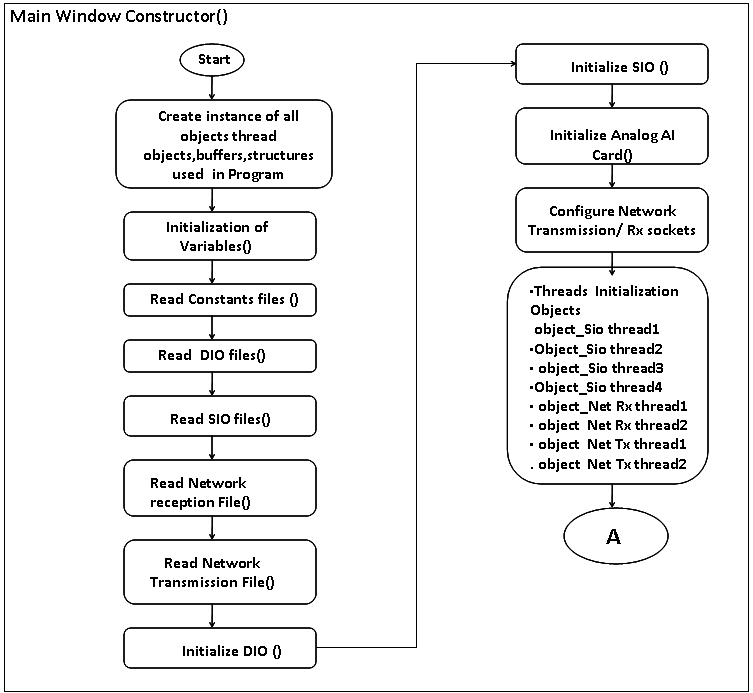
\includegraphics[width=\linewidth]{./FlowCharts/PngFlowCharts/Main1.png}
	%\caption{Five Chain Configuration of Telecommand}
	%\label{FIG:FiveChConfig}
\end{figure}
\begin{figure}[H]
	\centering
	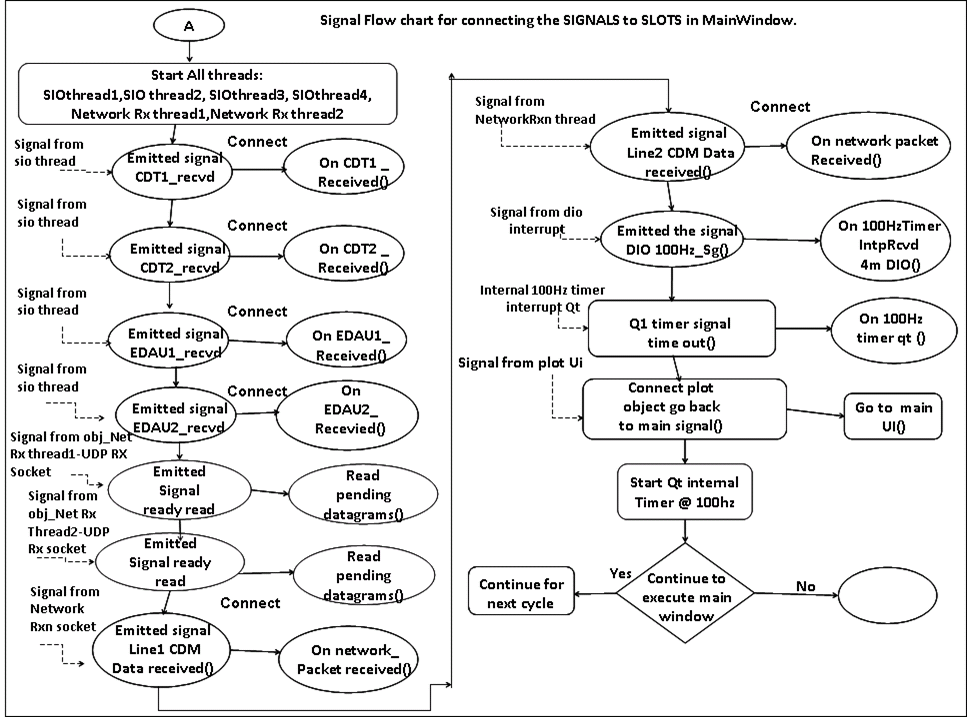
\includegraphics[width=\linewidth]{./FlowCharts/PngFlowCharts/Main2.png}
	%\caption{Five Chain Configuration of Telecommand}
	%\label{FIG:FiveChConfig}
\end{figure}
\section{Flow charts of slots in mainWindow}
\subsection{CDT Slot Flow Charts in mainWindow}

\begin{figure}[H]
	\centering
	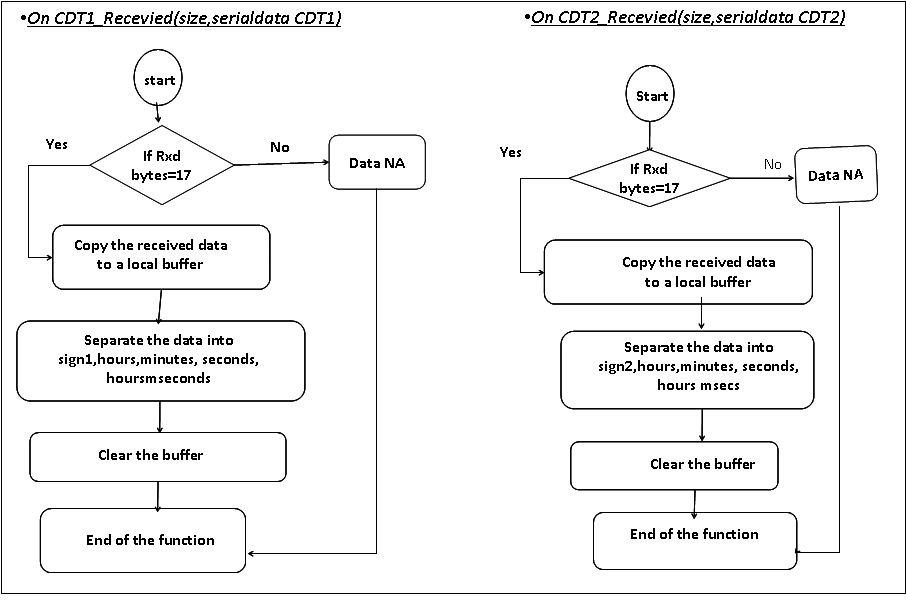
\includegraphics[width=\linewidth]{./FlowCharts/PngFlowCharts/SLOT_CDT12.png}
	%\caption{Five Chain Configuration of Telecommand}
	%\label{FIG:FiveChConfig}
\end{figure}
\subsection{EDAU Slot Flow Charts in mainWindow}

\begin{figure}[H]
	\centering
	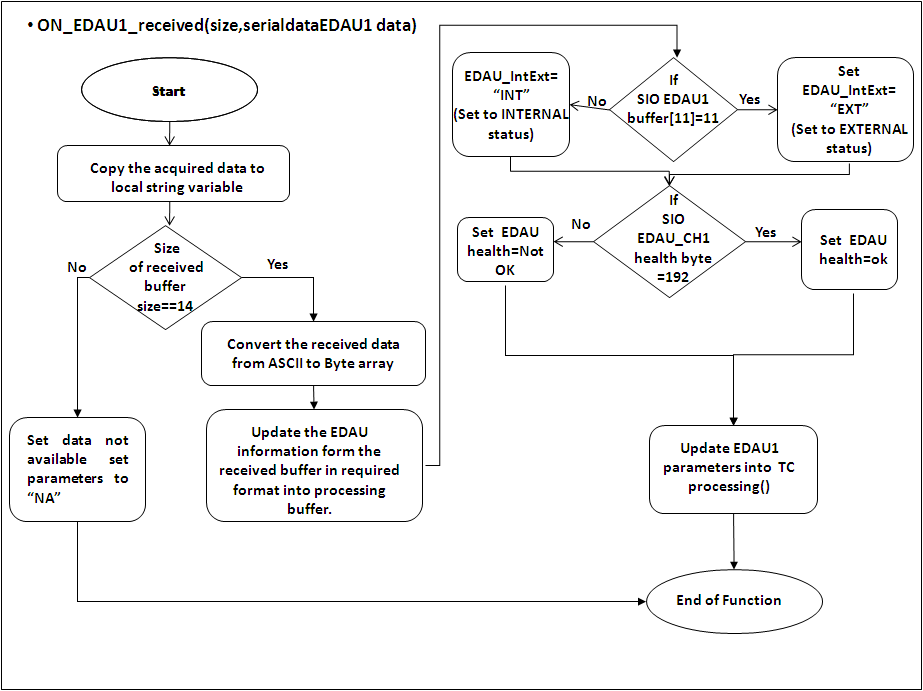
\includegraphics[width=\linewidth]{./FlowCharts/PngFlowCharts/SLOT_EDAU1.png}
	%\caption{Five Chain Configuration of Telecommand}
	%\label{FIG:FiveChConfig}
\end{figure}
\begin{figure}[H]
	\centering
	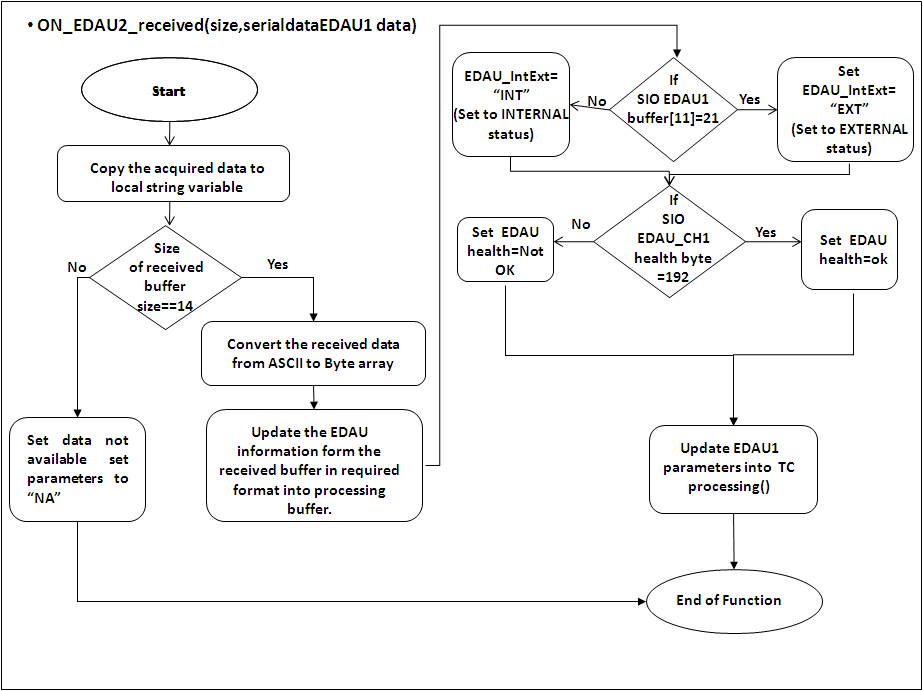
\includegraphics[width=\linewidth]{./FlowCharts/PngFlowCharts/SLOT_EDAU2.png}
	%\caption{Five Chain Configuration of Telecommand}
	%\label{FIG:FiveChConfig}
\end{figure}

\subsection{CDM Slot Charts in mainWindow}

\begin{figure}[H]
	\centering
	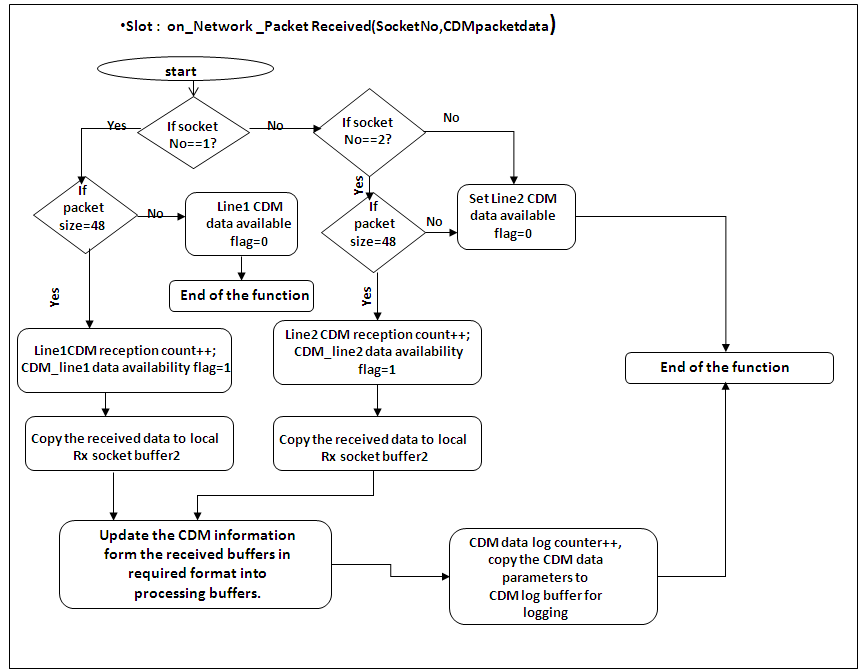
\includegraphics[width=\linewidth]{./FlowCharts/PngFlowCharts/SLOT_CDM.png}
	%\caption{Five Chain Configuration of Telecommand}
	%\label{FIG:FiveChConfig}
\end{figure}

\subsection{100Hz Interrupt received slot in mainWindow}
\begin{figure}[H]
	\centering
	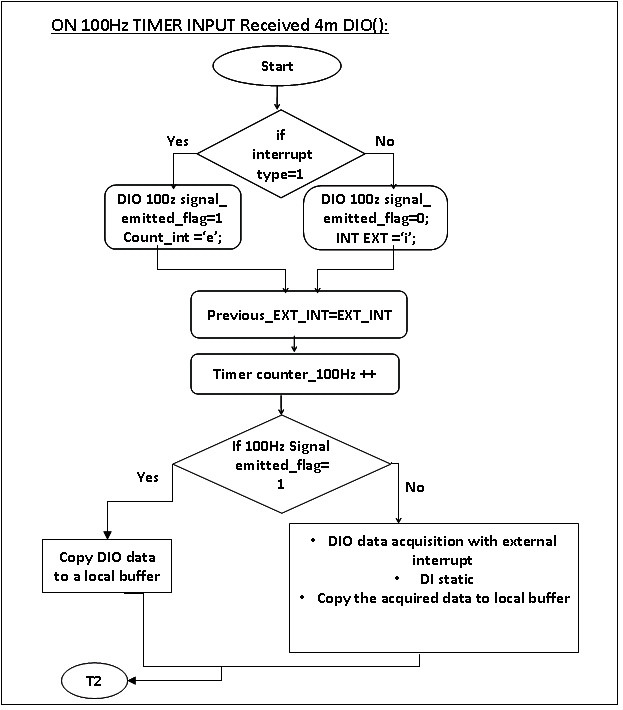
\includegraphics[width=\linewidth]{./FlowCharts/PngFlowCharts/SLOT_100Hz1.png} 
	%\caption{Five Chain Configuration of Telecommand}
	%\label{FIG:FiveChConfig}
\end{figure}
\begin{figure}[H]
	\centering
	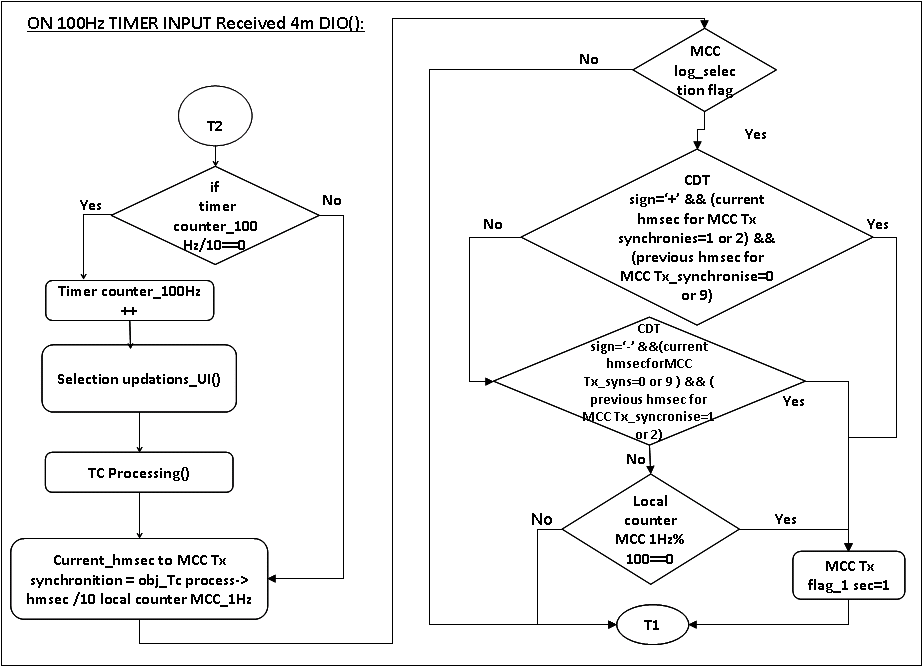
\includegraphics[width=\linewidth]{./FlowCharts/PngFlowCharts/SLOT_100Hz11.png} 
	%\caption{Five Chain Configuration of Telecommand}
	%\label{FIG:FiveChConfig}
\end{figure}
\begin{figure}[H]
	\centering
	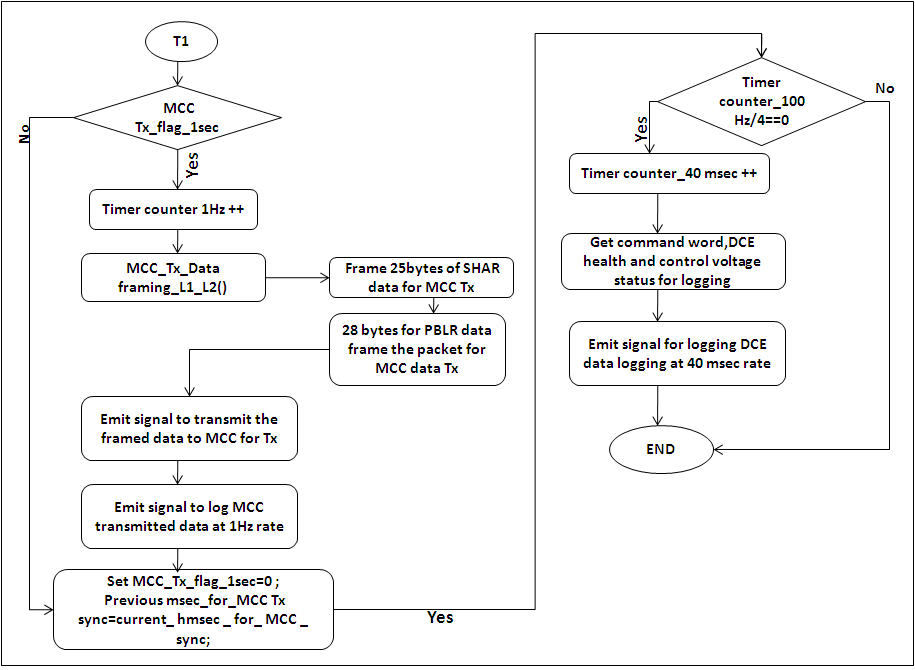
\includegraphics[width=\linewidth]{./FlowCharts/PngFlowCharts/SLOT_100Hz2.png} 
	%\caption{Five Chain Configuration of Telecommand}
	%\label{FIG:FiveChConfig}
\end{figure}

\subsection{TcProcess Flow charts: in mainWindow}

\begin{figure}[H]
	\centering
	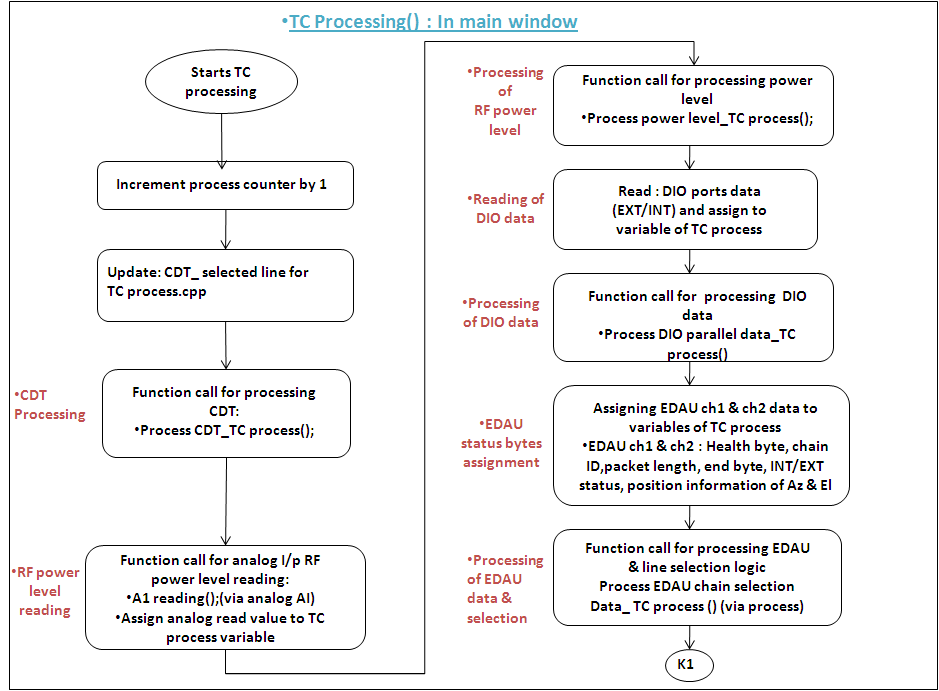
\includegraphics[width=\linewidth]{./FlowCharts/PngFlowCharts/TCP1.png}
	%\caption{Five Chain Configuration of Telecommand}
	%\label{FIG:FiveChConfig}
\end{figure}

\begin{figure}[H]
	\centering
	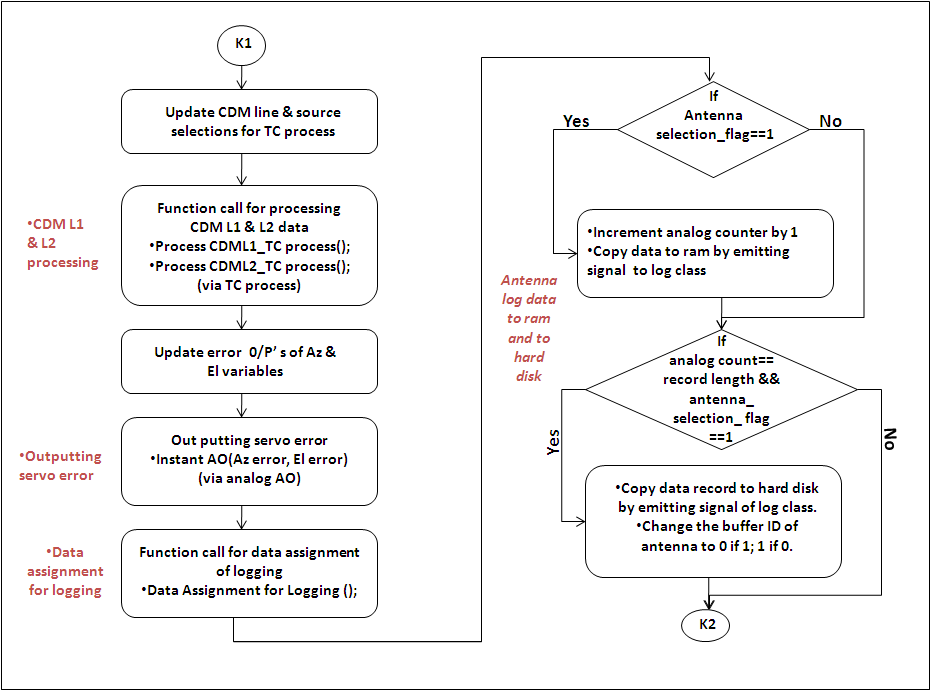
\includegraphics[width=\linewidth]{./FlowCharts/PngFlowCharts/TCP2.png}
	%\caption{Five Chain Configuration of Telecommand}
	%\label{FIG:FiveChConfig}
\end{figure}

\begin{figure}[H]
	\centering
	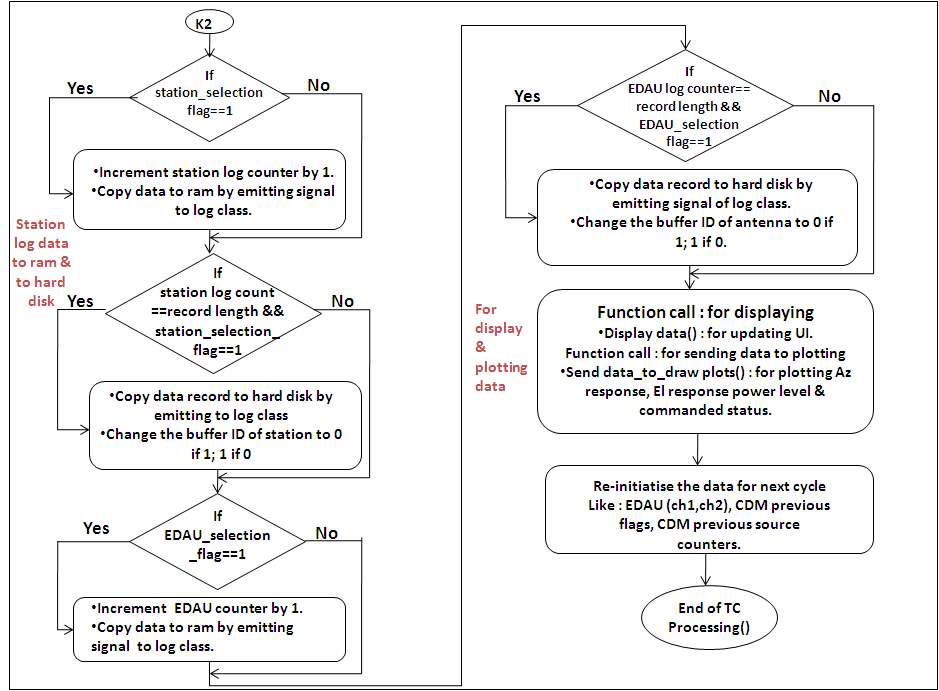
\includegraphics[width=\linewidth]{./FlowCharts/PngFlowCharts/TCP3.png}
	%\caption{Five Chain Configuration of Telecommand}
	%\label{FIG:FiveChConfig}
\end{figure}
\subsection{Data assignment for logging: in mainWindow}
\begin{figure}[H]
	\centering
	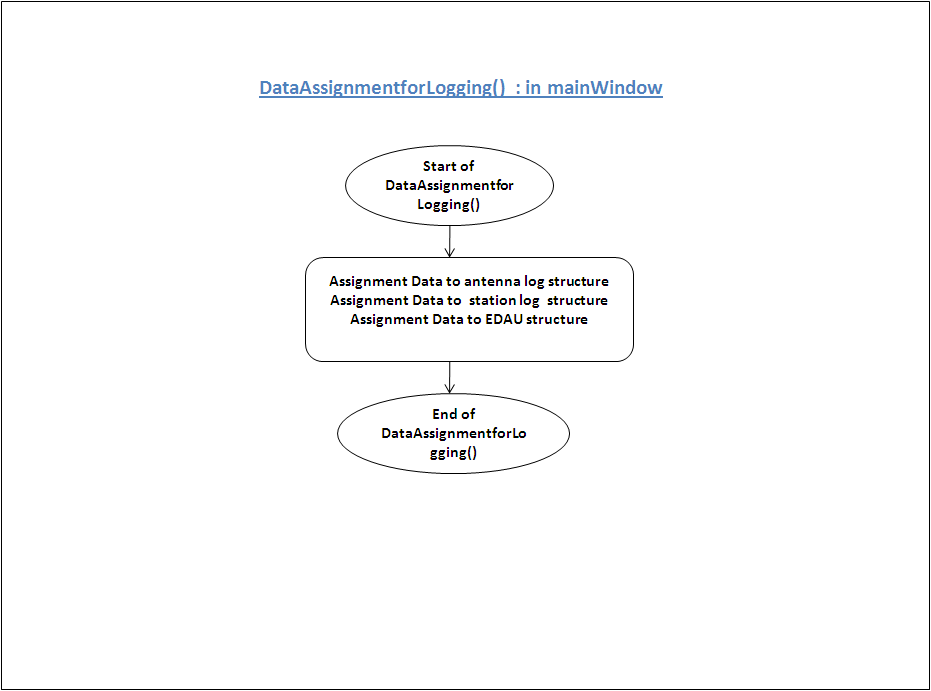
\includegraphics[width=\linewidth]{./FlowCharts/PngFlowCharts/TCP11.png}
	%\caption{Five Chain Configuration of Telecommand}
	%\label{FIG:FiveChConfig}
\end{figure}
\section{TC process flow charts : tcprocess class}
\subsection{CDT Processing}
\begin{figure}[H]
	\centering
	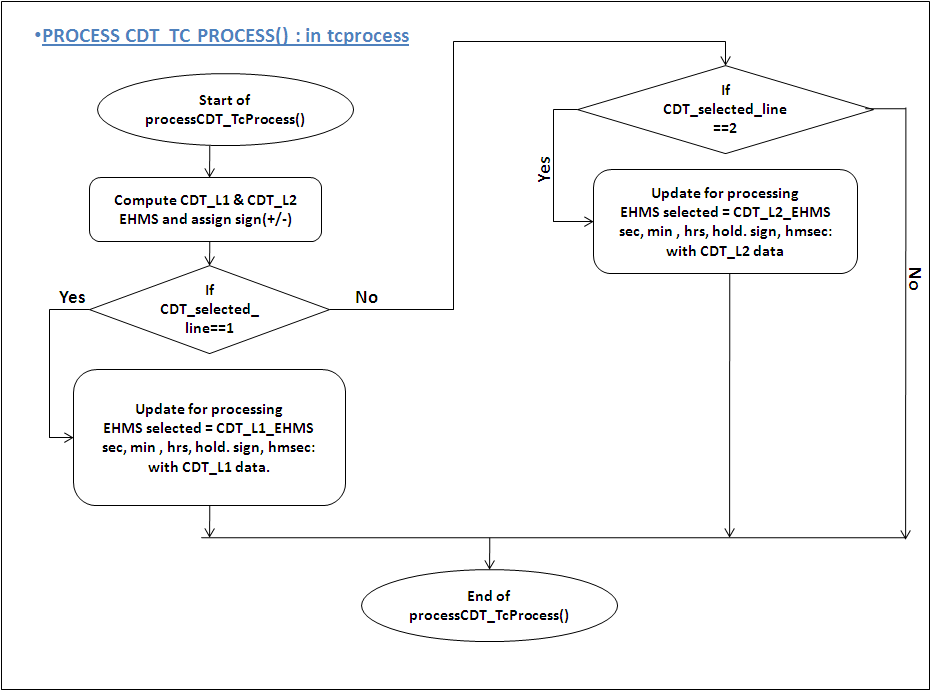
\includegraphics[width=\linewidth]{./FlowCharts/PngFlowCharts/TCP4.png}
	%\caption{Five Chain Configuration of Telecommand}
	%\label{FIG:FiveChConfig}
\end{figure}
\subsection{RF power level processing}
\begin{figure}[H]
	\centering
	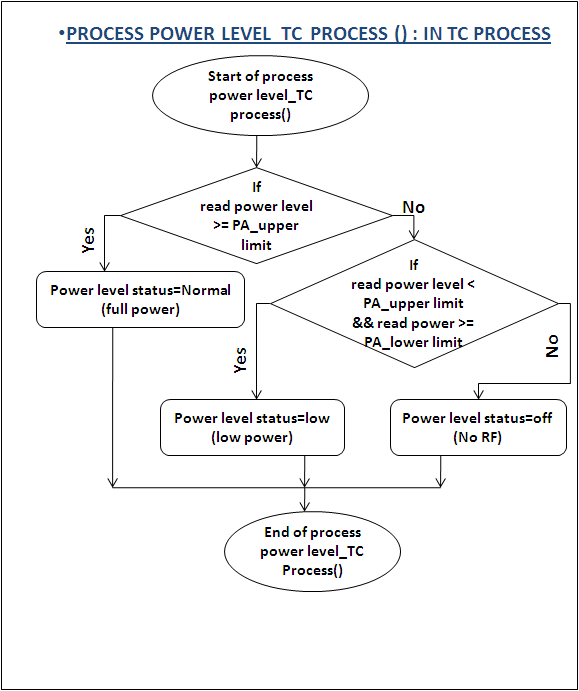
\includegraphics[width=\linewidth]{./FlowCharts/PngFlowCharts/TC_PA.png}
	%\caption{Five Chain Configuration of Telecommand}
	%\label{FIG:FiveChConfig}
\end{figure}

\subsection{DIO parallel data processing}
\begin{figure}[H]
	\centering
	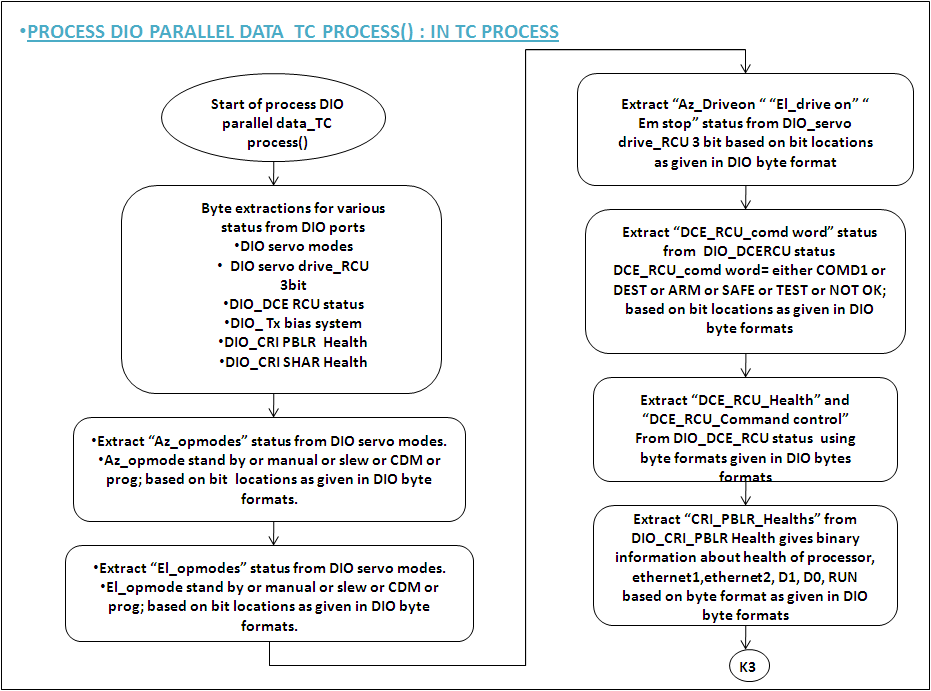
\includegraphics[width=\linewidth]{./FlowCharts/PngFlowCharts/TCP6.png}
	%\caption{Five Chain Configuration of Telecommand}
	%\label{FIG:FiveChConfig}
\end{figure}

\begin{figure}[H]
	\centering
	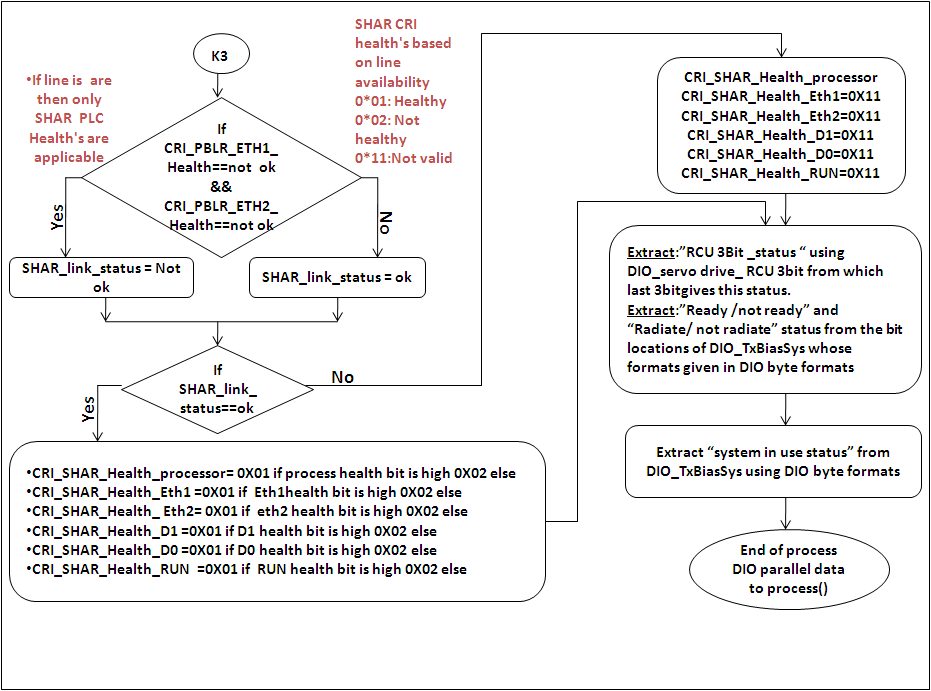
\includegraphics[width=\linewidth]{./FlowCharts/PngFlowCharts/TCP7.png}
	%\caption{Five Chain Configuration of Telecommand}
	%\label{FIG:FiveChConfig}
\end{figure}

\subsection{CDM data processing}
\begin{figure}[H]
	\centering
	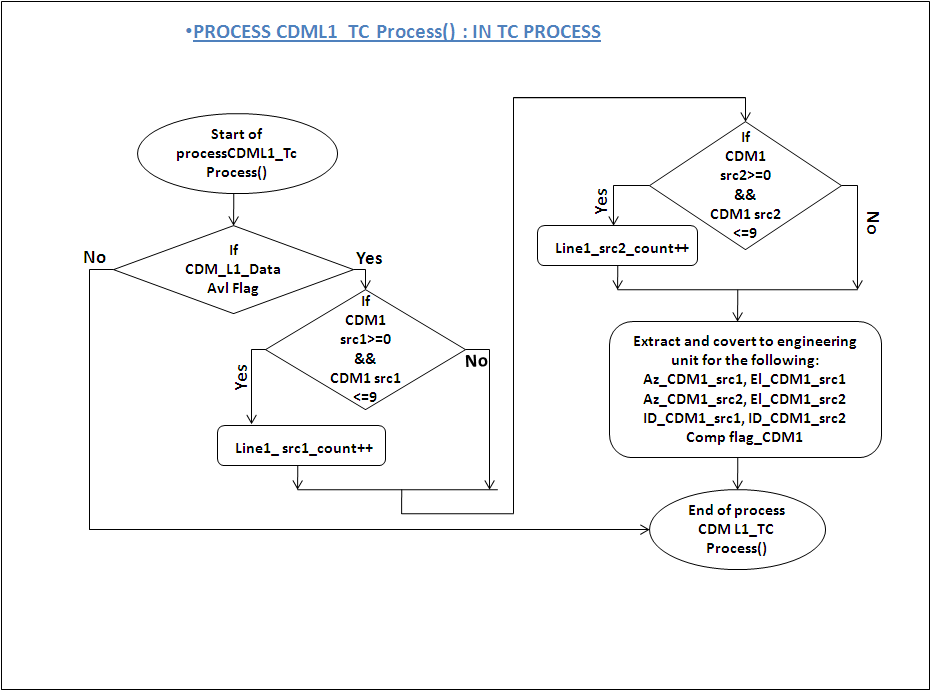
\includegraphics[width=\linewidth]{./FlowCharts/PngFlowCharts/TCP8.png}
	%\caption{Five Chain Configuration of Telecommand}
	%\label{FIG:FiveChConfig}
\end{figure}

\begin{figure}[H]
	\centering
	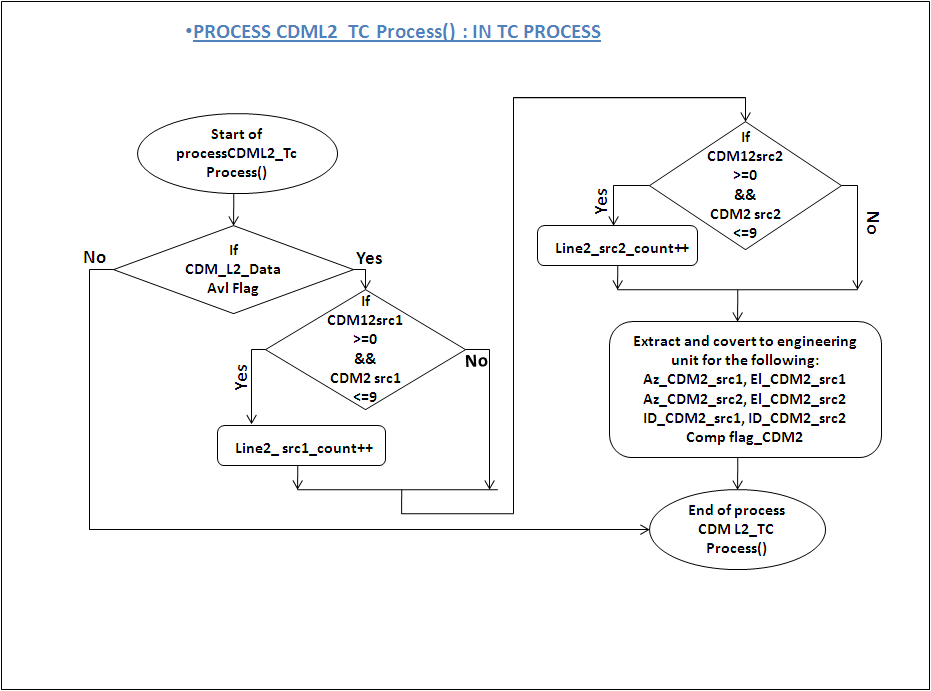
\includegraphics[width=\linewidth]{./FlowCharts/PngFlowCharts/TCP9.png}
	%\caption{Five Chain Configuration of Telecommand}
	%\label{FIG:FiveChConfig}
\end{figure}

\subsection{EDAU flow charts}
\begin{figure}[H]
	\centering
	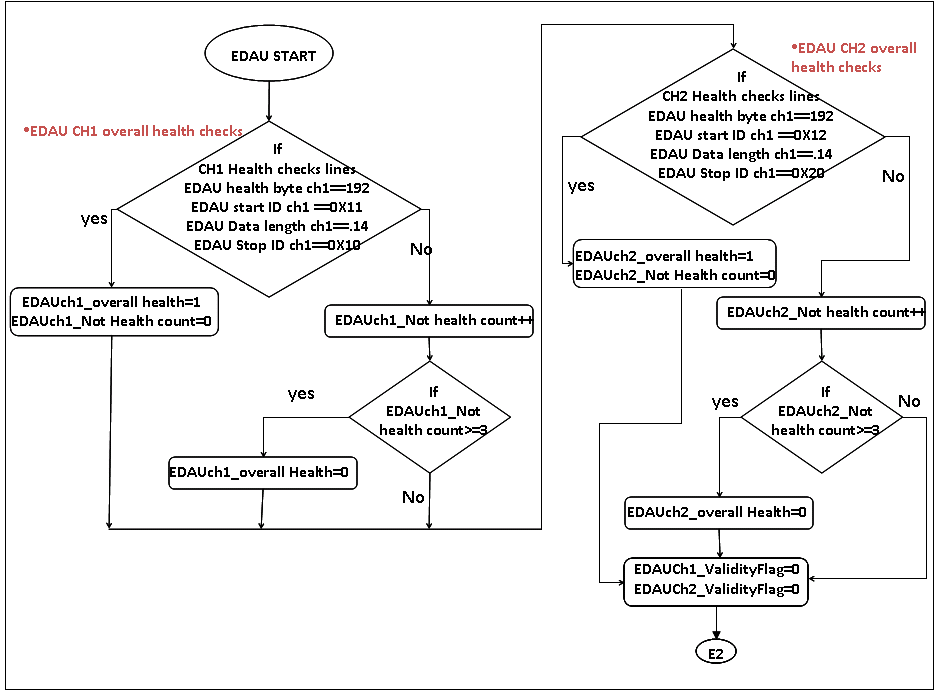
\includegraphics[width=\linewidth]{./FlowCharts/PngFlowCharts/EDAU1.png}
	%\caption{Five Chain Configuration of Telecommand}
	%\label{FIG:FiveChConfig}
\end{figure}

\begin{figure}[H]
	\centering
	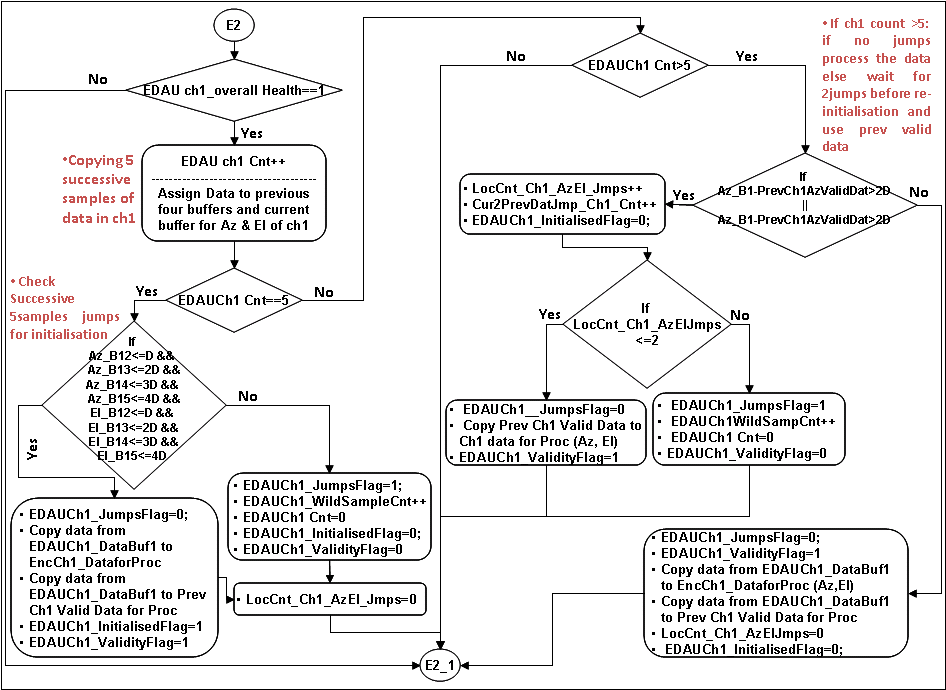
\includegraphics[width=\linewidth]{./FlowCharts/PngFlowCharts/EDAU2.png}
	%\caption{Five Chain Configuration of Telecommand}
	%\label{FIG:FiveChConfig}
\end{figure}

\begin{figure}[H]
	\centering
	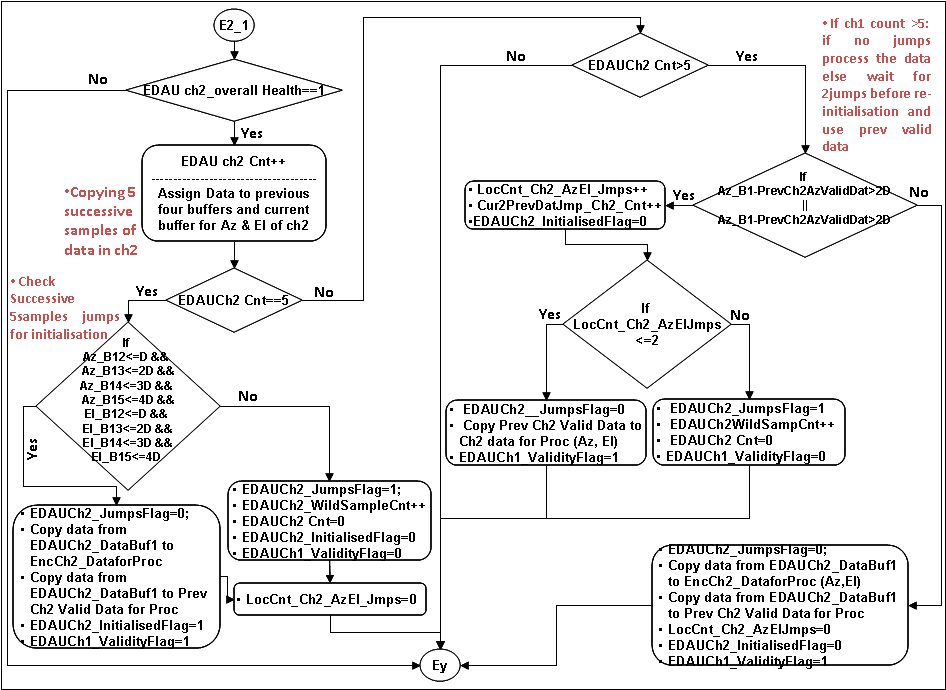
\includegraphics[width=\linewidth]{./FlowCharts/PngFlowCharts/EDAU3.png}
	%\caption{Five Chain Configuration of Telecommand}
	%\label{FIG:FiveChConfig}
\end{figure}

\begin{figure}[H]
	\centering
	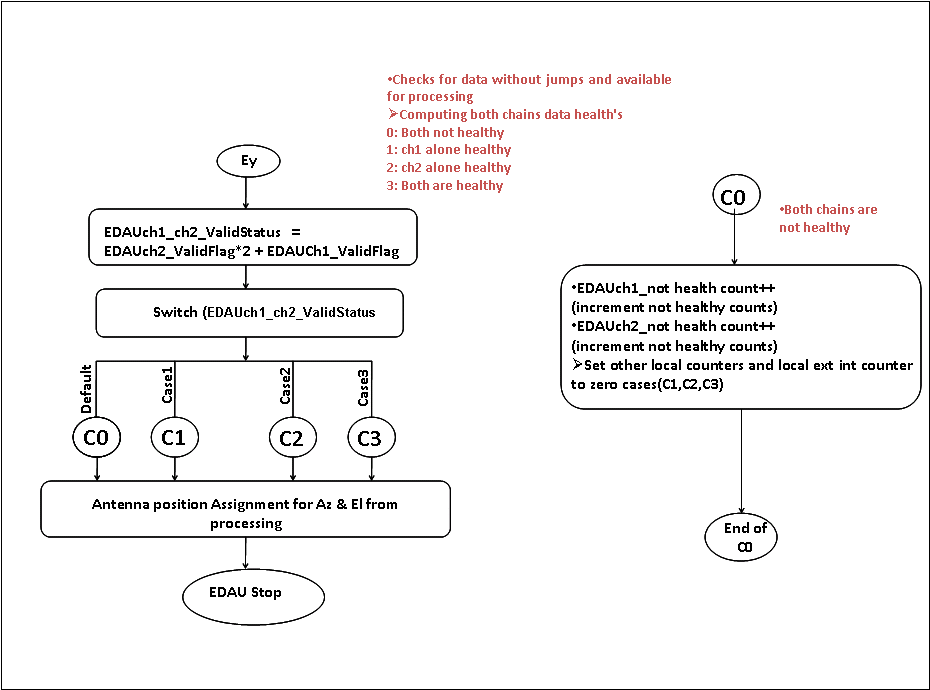
\includegraphics[width=\linewidth]{./FlowCharts/PngFlowCharts/EDAU5.png}
	%\caption{Five Chain Configuration of Telecommand}
	%\label{FIG:FiveChConfig}
\end{figure}


\begin{figure}[H]
	\centering
	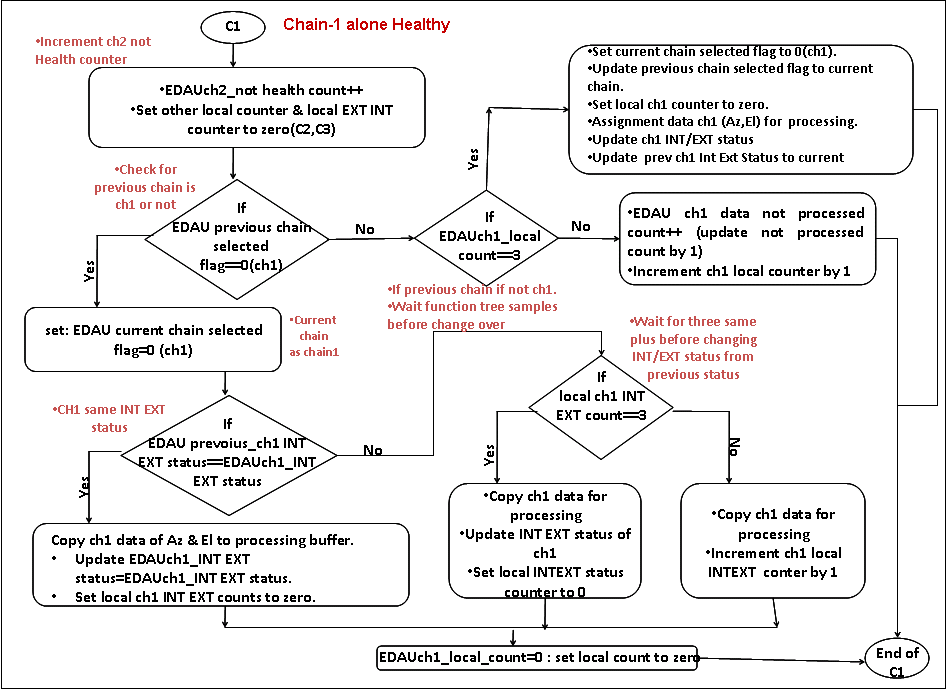
\includegraphics[width=\linewidth]{./FlowCharts/PngFlowCharts/EDAU6.png}
	%\caption{Five Chain Configuration of Telecommand}
	%\label{FIG:FiveChConfig}
\end{figure}


\begin{figure}[H]
	\centering
	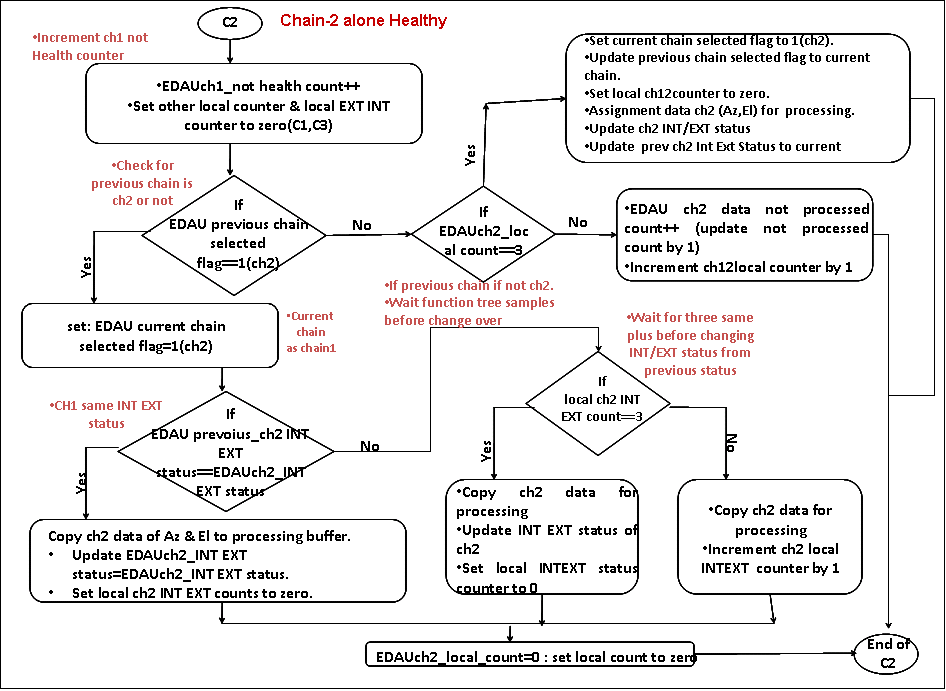
\includegraphics[width=\linewidth]{./FlowCharts/PngFlowCharts/EDAU7.png}
	%\caption{Five Chain Configuration of Telecommand}
	%\label{FIG:FiveChConfig}
\end{figure}


\begin{figure}[H]
	\centering
	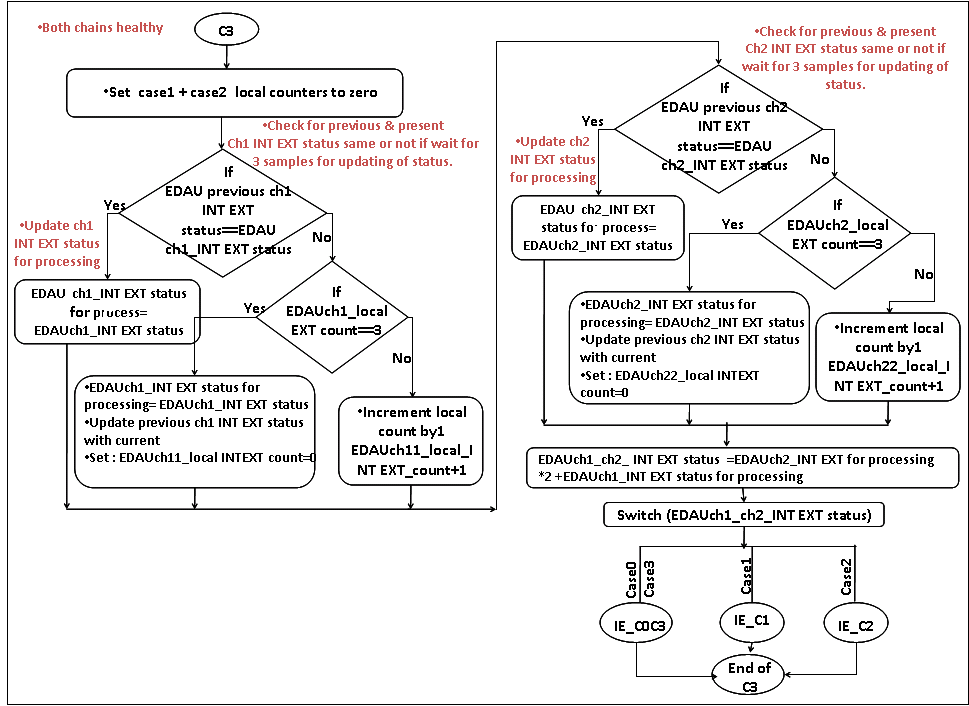
\includegraphics[width=\linewidth]{./FlowCharts/PngFlowCharts/EDAU8.png}
	%\caption{Five Chain Configuration of Telecommand}
	%\label{FIG:FiveChConfig}
\end{figure}


\begin{figure}[H]
	\centering
	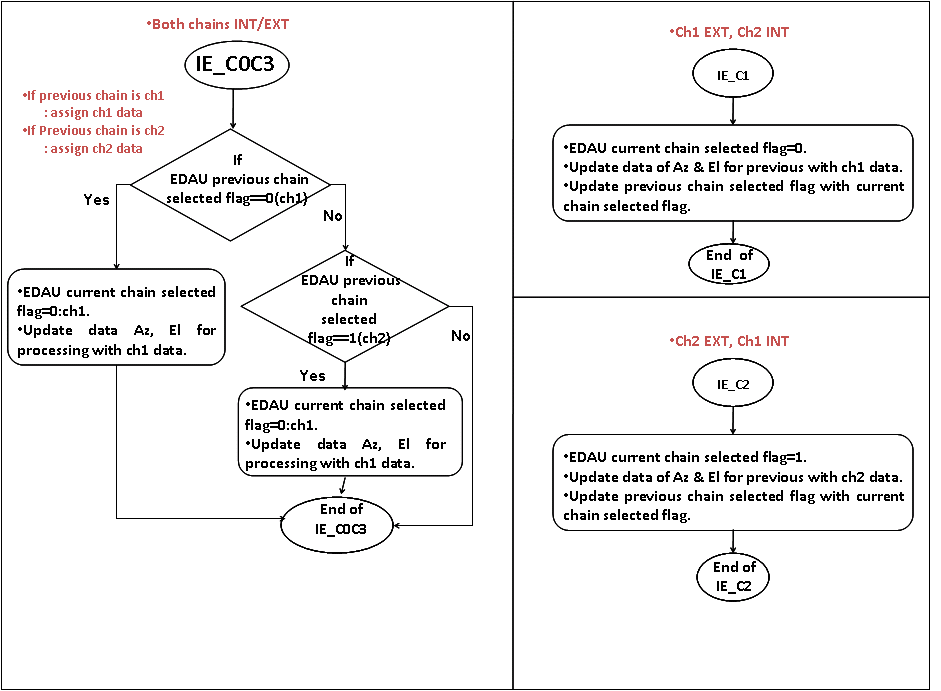
\includegraphics[width=\linewidth]{./FlowCharts/PngFlowCharts/EDAU9.png}
	%\caption{Five Chain Configuration of Telecommand}
	%\label{FIG:FiveChConfig}
\end{figure}




% *************** TC Process Flow charts *******
\section{Analog data input and output}
\subsection{Analog output}
\begin{figure}[H]
	\centering
	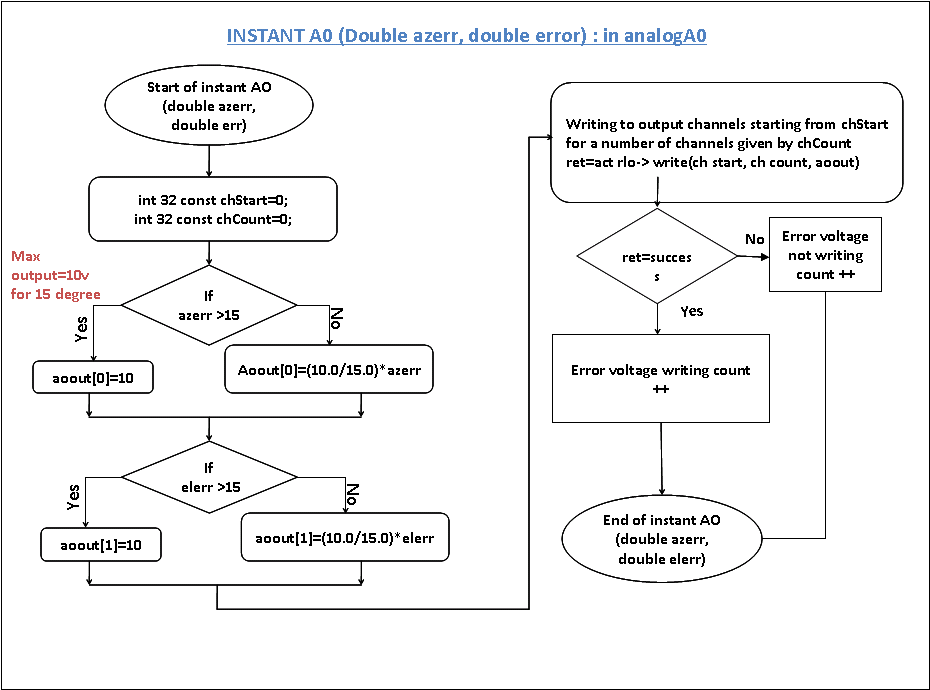
\includegraphics[width=\linewidth]{./FlowCharts/PngFlowCharts/TCP10.png}
\end{figure}
\subsection{Analog input}
\begin{figure}[H]
	\centering
	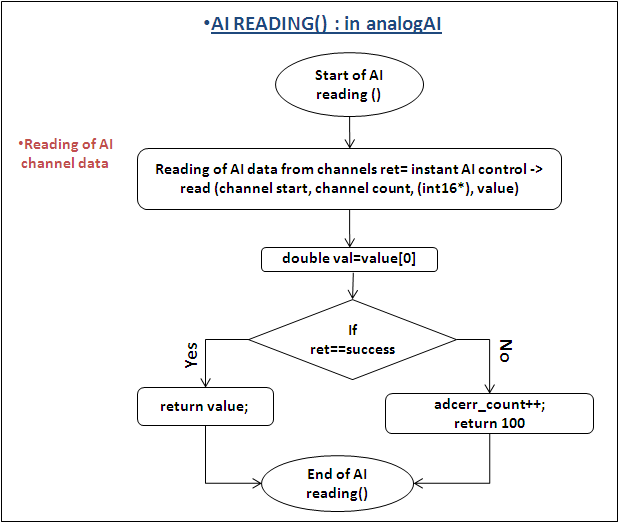
\includegraphics[width=\linewidth]{./FlowCharts/PngFlowCharts/AnalogInput.png}
\end{figure}
\section{Flow charts for concurrent data flow}
\subsection{EDAU serial data reception}
\begin{figure}[H]
	\centering
	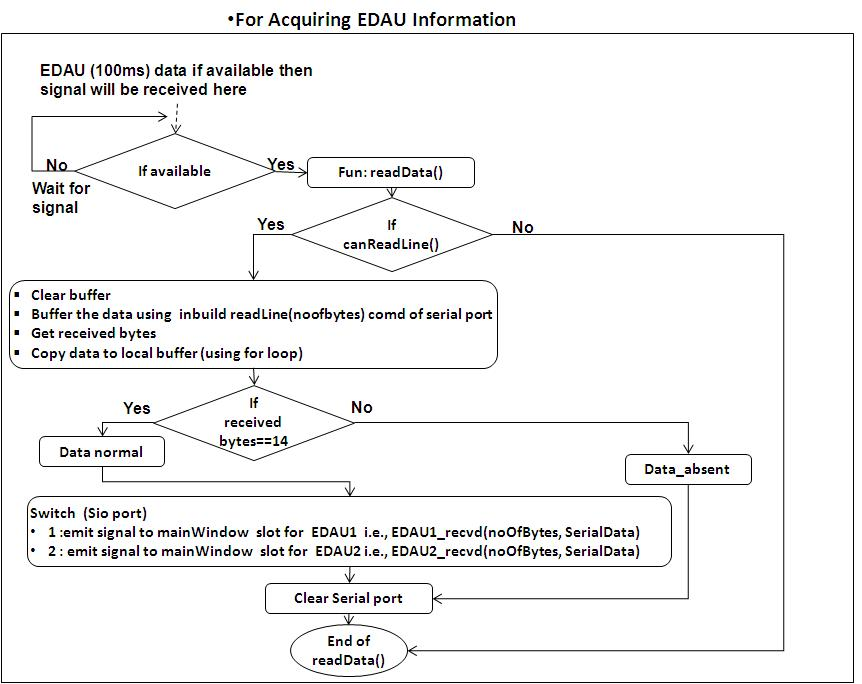
\includegraphics[width=\linewidth]{./FlowCharts/PngFlowCharts/SG1_EDAU.png}
	%\caption{Five Chain Configuration of Telecommand}
	%\label{FIG:FiveChConfig}
\end{figure}
\subsection{CDT serial data reception}
\begin{figure}[H]
	\centering
	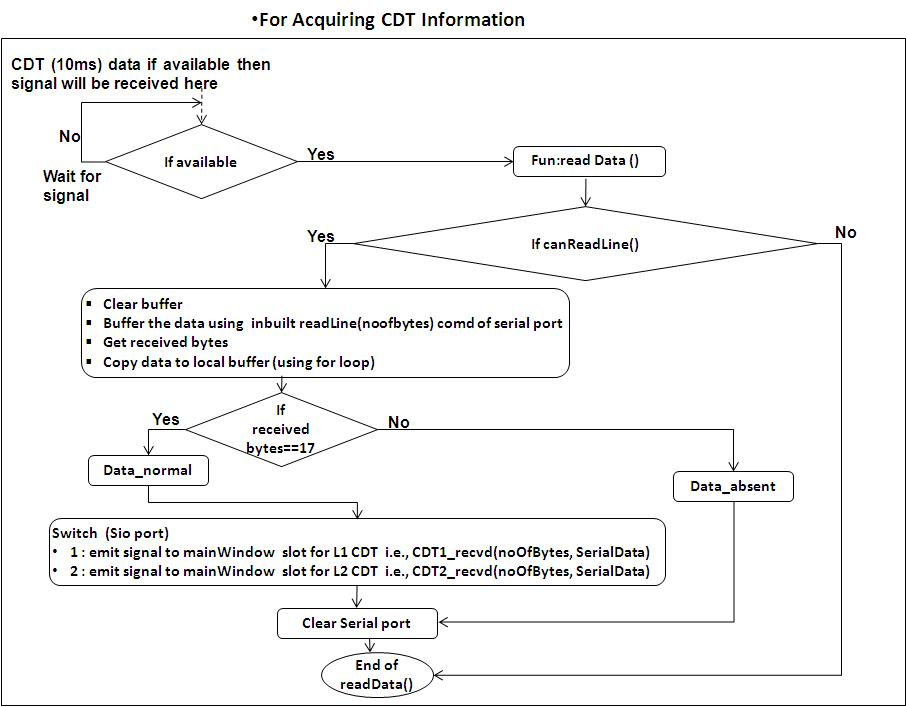
\includegraphics[width=\linewidth]{./FlowCharts/PngFlowCharts/SG2_CDT.png}
	%\caption{Five Chain Configuration of Telecommand}
	%\label{FIG:FiveChConfig}
\end{figure}
\subsection{CDM network reception}
\begin{figure}[H]
	\centering
	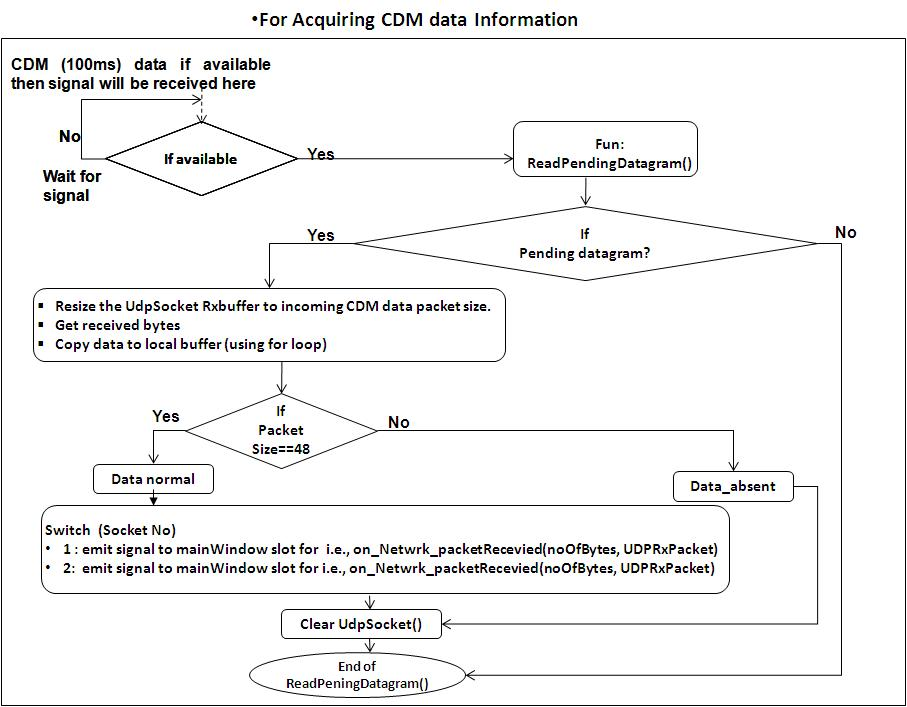
\includegraphics[width=\linewidth]{./FlowCharts/PngFlowCharts/SG3_CDM.png}
	%\caption{Five Chain Configuration of Telecommand}
	%\label{FIG:FiveChConfig}
\end{figure}
\subsection{DI parallel interrupt}
\begin{figure}[H]
	\centering
	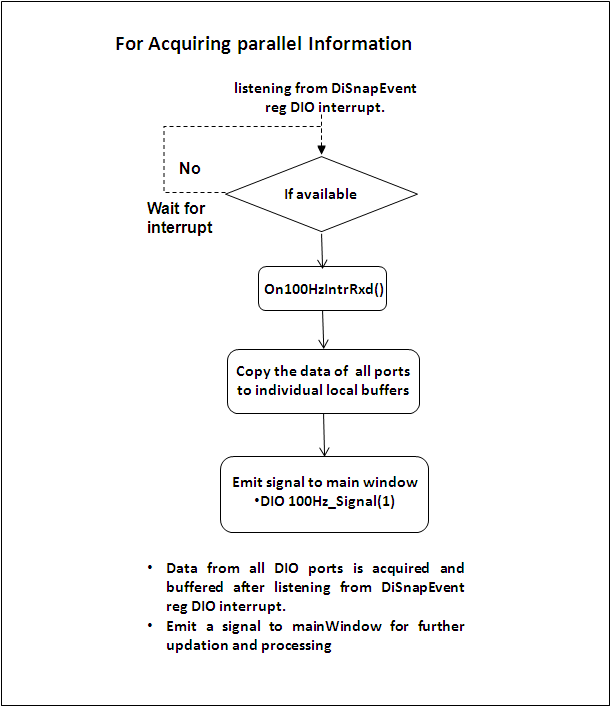
\includegraphics[width=\linewidth]{./FlowCharts/PngFlowCharts/SG4_DIO.png}
	%\caption{Five Chain Configuration of Telecommand}
	%\label{FIG:FiveChConfig}
\end{figure}
\chapter{Features of new Linux based DPS compared to old windows 2K based DPS}\label{Chapter9}


\begin{enumerate}
	\item [$\blacksquare$] Continuous logging at different rates. DCE/RCU logging is introduced as per project requirement for logging the DCE/RCU data at 40ms rate via DI interface.
	\item [$\blacksquare$] Radiated power level limits (lower and upper) are configurable through tcconstants.inp file where as these are hardcoded in windows based DPS. 
	\item [$\blacksquare$] Independent buffers for line-1 and line-2 of MCC are maintained and logged independently where as single buffer was in use for windows based DPS. 
	\item [$\blacksquare$] Programmable limits and pre-limits are provided for both azimuth and elevation in-addition to mechanical limits. Only mechanical limts and pre-limits are available for windows based DPS. 
	\item [$\blacksquare$] Application developed caters the need for both SHAR and PBLR TC chains. Only corresponding input files (rxsocket, txsocket, sio, pio, constants) to be changed as per chain configuration. 
	\item [$\blacksquare$] Healths of add on cards along with threads running status is provided on the main GUI page. This information is not available in windows based DPS.
	\item [$\blacksquare$] Plotting is introduced in the new design. In this azimuth and elevation responses are plotted in two segments. Power level status and command radiated status are plotted in other two segments of second GUI plotting page.
	\item [$\blacksquare$] Logged data are saved into harddisk and the folder name as specified in the tcconstants file. This is not there in windows based DPS.
	\item [$\blacksquare$] Timing data is acquired in two chains one each from two readers using RS232 serial interface at refresh rate of 10ms. This has reduced the load on DI card compared to windows based DPS, where in CDT is acquired using DI card for BCD timing data. 
	\item [$\blacksquare$] The limitation of windows based DPS for prog mode data is taken care in the new design. In the old design, prog mode data takes upto T+500s and after that in case of selection of prog mode (operational error), antenna will run away to initial position. In the new linux based DPS, prog mode data takes upto T+1000s and after that also incase of selection of prog mode, commanded angle takes the last value at T+1000s. Also, in case of non availability of prog mode data before T+1000s previous value will be buffered for the rest of the values. 
	\item [$\blacksquare$] Extra parameters are added in different log files and each log file is provided with header containing the information of the parameters being logged.
	\item [$\blacksquare$] Default logging for all files is incorporated as per suggestion of STARS. MCC transmission and logging is selection dependant by the operator. CDM data will be logged as and when data is received. In windows based DPS, defulat logging is off and MCC transmission is on.  
\end{enumerate}
\chapter{Display Pages}
\label{Chapter10}
The software product contains two GUI pages. Main display page (status and selection page) and second display page (plotting page).
Main display page as shown in \ref{FIG:DPSMainPage} provides status of different sub-systems, functionality of different add on cards along with threads running status, various log counters, packets counters for MCC and RSP, pushbuttons for selections (logging, timing information, CDM sources) and enabling of plotting in secondary GUI along with switch over option to 2nd GUI page. \newline

Second display play is divided into four segments and is provided with a pushbutton for switching over to main GUI page. This second GUI page is shown in \ref{FIG:DPSSecondPage}. Segments are arranged in an array of 2$\times$2. At (0,0) azimuth response is plotted containing commanded angle and antenna position on primary y-axis and corresponding error on secondary y-axis. The plotting is done with reference to CDT on x-axis. Similarly, at (0,1) elevation response is plotted containing commanded angle and antenna position on primary y-axis and corresponding error on secondary y-axis. The plotting is done with reference to CDT on x-axis. Transmitter RF output power level status is displayed on primary y-axis with reference to CDT on x-axis and this is plotted in segment (1,0). Finally, the segment (1,1) contains radiated command word status on y-axis with reference to CDT on x-axis.

\begin{figure}[H]
	\centering
	\includegraphics[height=1.2\linewidth, width=\linewidth]{./Diagrams/MainPage.png}
	\caption{DPS Main Page}
	\label{FIG:DPSMainPage}
\end{figure}
	   

\begin{figure}[H]
	\centering
	\includegraphics[height=1.2\linewidth, width=\linewidth]{./Diagrams/SecondaryPage.png}
	\caption{DPS Secondary Page}
	\label{FIG:DPSSecondPage}
\end{figure}
% Bibliography
%\chapter{Bibliography}
\begin{thebibliography}{99}
\bibitem{TCOldSWDoc} PC based Application software for Telecommand MKIII design document.
\bibitem{TCOldStnMan} Telecommand Station Manual
\bibitem{CRISWDoc} Software Design Description: Command Remote Interface 
for Portblair Telecommand Station ::CRI SHAR-CRI PBLR

\bibitem{CRISRS} Software Requirements Specification: Command Remote Interface for Portblair Telecommand Station

\bibitem{SYRSLBDPS} System Requirements Specification document for Linux Based DPS of Telecommand Data Systems

\bibitem{SRSLBDPS} Software Requirements Specification document for Linux Based DPS of Telecommand Data Systems

% #######################  18 : next 19 #######################



\end{thebibliography}% Bibliography
%% ----------------------------------------------------------------
% Now begin the Appendices, including them as separate files
\addtocontents{toc}{\vspace{0em}}
\backmatter
%\chapter{Display Pages}
\label{Chapter10}
The software product contains two GUI pages. Main display page (status and selection page) and second display page (plotting page).
Main display page as shown in \ref{FIG:DPSMainPage} provides status of different sub-systems, functionality of different add on cards along with threads running status, various log counters, packets counters for MCC and RSP, pushbuttons for selections (logging, timing information, CDM sources) and enabling of plotting in secondary GUI along with switch over option to 2nd GUI page. \newline

Second display play is divided into four segments and is provided with a pushbutton for switching over to main GUI page. This second GUI page is shown in \ref{FIG:DPSSecondPage}. Segments are arranged in an array of 2$\times$2. At (0,0) azimuth response is plotted containing commanded angle and antenna position on primary y-axis and corresponding error on secondary y-axis. The plotting is done with reference to CDT on x-axis. Similarly, at (0,1) elevation response is plotted containing commanded angle and antenna position on primary y-axis and corresponding error on secondary y-axis. The plotting is done with reference to CDT on x-axis. Transmitter RF output power level status is displayed on primary y-axis with reference to CDT on x-axis and this is plotted in segment (1,0). Finally, the segment (1,1) contains radiated command word status on y-axis with reference to CDT on x-axis.

\begin{figure}[H]
	\centering
	\includegraphics[height=1.2\linewidth, width=\linewidth]{./Diagrams/MainPage.png}
	\caption{DPS Main Page}
	\label{FIG:DPSMainPage}
\end{figure}
	   

\begin{figure}[H]
	\centering
	\includegraphics[height=1.2\linewidth, width=\linewidth]{./Diagrams/SecondaryPage.png}
	\caption{DPS Secondary Page}
	\label{FIG:DPSSecondPage}
\end{figure}% Paper submission and statuses


%\newpage
%\addtocontents{toc}{\vspace{2em}}
%\backmatter
%\section*{Papers}
%\label{Chapt10}
%\begin{enumerate}
%\item[$\blacksquare$] Under publication
%	\begin{enumerate}
%		\item[1.] ``A Robust Digital Image Watermarking  technique using auto encoder based Convolutional Neural Networks", Submitted to ``IEEE workshop on Computational Intelligence : Theories, Applications and 		Future Directions (IEEEWCI-2015) at IIT Kanpur" and accepted for publication.
%	\end{enumerate}
%\item[$\blacksquare$] Under review
%	\begin{enumerate}
% 	    \item[1.] ``Exploring the Learning Capabilities of Convolutional Neural Networks for Robust Image Watermarking", Submitted to : Computers $\&$ Security, Elsevier.
%	\end{enumerate}
%\item[$\blacksquare$] Under preparation
%	\begin{enumerate}
%		\item[1.] ``Incorporating Rotational Invariance for Convolutional Neural Network Architecture", Report under preparation. 
%		\item[2.] ``Deep learning networks for microfluidics based cytopathology analysis", Report under preparation. 
%		%Submitted to : Pattern Recognition, Elsevier. 
%	\end{enumerate}
%\end{enumerate} 


\addtocontents{toc}{\vspace{1.5em}} % Add a gap in the Contents, for aesthetics

\appendix % Cue to tell LaTeX that the following 'chapters' are Appendices

%\chapter{An Appendix}

\section()	% Appendix Title

%\input{Appendices/AppendixB} % Appendix Title

%\input{Appendices/AppendixC} % Appendix Title

\addtocontents{toc}{\vspace{1.5em}}  % Add a gap in the Contents, for aesthetics
%\backmatter

%% ----------------------------------------------------------------
%\label{Bibliography}
%\%lhead{\emph{Bibliography}}  % Change the left side page header 	to "Bibliography"
%\bibliographystyle{plain}  % Use the "unsrtnat" BibTeX style for formatting the Bibliography
%\bibliography{bibo}  % The references (bibliography) information are stored in the file named "Bibliography.bib"

\end{document}  % The End
%%	 ----------------------------------------------------------------
